\documentclass[11pt,letterpaper,twoside]{report}

% Layout
\usepackage{geometry}
\usepackage{setspace}
\usepackage{titlesec}
\usepackage{tocloft}
\usepackage[hang,flushmargin]{footmisc}

% Citation style
% \usepackage{harvard}
\usepackage[natbibapa]{apacite}         % Citation Style
\usepackage{endnotes}

% Figures
\usepackage{graphicx}
\usepackage{grffile}
\usepackage{subcaption}
\usepackage{epsfig}
\usepackage{multicol}
\usepackage{listings}
\usepackage{rotating}                   % Figure rotation
\usepackage{floatrow}                   % Can only pick one of: float, floatrow
\floatsetup[figure]{capposition=top}    % Specify where to put FIGURE caption
\usepackage[labelfont=bf]{caption}      % Table/Figure bold caption


% Tables
% \usepackage{booktabs}
% \usepackage{dcolumn}
% \usepackage{multirow}
% \usepackage{hhline}
% \usepackage{stackengine}
% \usepackage{tablefootnote}
\usepackage{tabularx}                   % Table formatting
\usepackage{multirow}                   % Table formatting 
\usepackage{multicol}                   % Table formatting
\usepackage{threeparttable}             % Tables with footnotes
\usepackage{lscape}                     % Table rotation
\usepackage[table]{xcolor}              % Table cell shading
\usepackage[labelfont=bf]{caption}      % Table/Figure bold caption
\floatsetup[table]{capposition=top}     % Specify where to put TABLE caption

% Algorithms
\usepackage[boxed,longend]{algorithm2e}

% Math
\usepackage{amsmath}
\usepackage{amssymb}
\usepackage{mathtools}
\usepackage{bbm}                        % Indicator function

% Typography
\usepackage{times}
\usepackage{microtype}
\usepackage{textcomp}
\usepackage[super]{nth}                 % Enables writing 1st, 2nd, etc.

% Macro support
\usepackage{xspace}
\usepackage{color}
\usepackage{ntheorem}

% Diagrams
\usepackage{pgf}
\usepackage{tikz} % extensive form game trees
\usetikzlibrary{calc} % calculating TikZ coordinates
\usetikzlibrary{arrows.meta} % arrows for theory diagrams
\usetikzlibrary{trees}

% PDF links
\usepackage[hidelinks]{hyperref} % backref=page




% Use proper margins.
\geometry{letterpaper,left=1.25in,top=1in,right=1.25in,bottom=1in,nohead}



% double-space text
\doublespacing

% Center chapter titles
% Place chapter title, number, and name on same line
% Make chapter headings all uppercase, standard font size
% Omit page numbers (RJN: I don't think I want this, commented out)
% \titleformat{\chapter}[hang]{\normalfont\fillast\bfseries}{\MakeUppercase{\chaptertitlename} \thechapter: }{0em}{\MakeUppercase}[\thispagestyle{empty}] % ORIGINAL
\titleformat{\chapter}[hang]{\normalfont\fillast\bfseries}{\MakeUppercase{\chaptertitlename} \thechapter: }{0em}{\MakeUppercase} % RJN edit

% Make section headings normal font size, bold
\titleformat*{\section}{\normalfont\bfseries}
\titleformat*{\subsection}{\normalfont\bfseries}
\titleformat*{\subsubsection}{\normalfont\bfseries}

% Extend to 2in top margins for chapter headings
\titlespacing{\chapter}{0in}{0.62in}{11pt}

% Indent paragraphs four spaces throughout the thesis/dissertation.
\setlength{\parindent}{4ex}

% Tweak spacing of paragraph labels.
\titlespacing{\paragraph}{0in}{0.08in}{0.07in}

% We want numbered subsubsections
\setcounter{secnumdepth}{3}
\setcounter{tocdepth}{3}

% We need to double-space between footnotes.
\setlength{\footnotesep}{13pt}

% Footnotes only one point smaller than text
\renewcommand{\footnotesize}{\small}

% We don't want crazy vertical spacing.
\raggedbottom

% We don't want abandoned words.
\clubpenalty=10000 
\widowpenalty=10000

% Prevent awkward hyphenations.
\hyphenation{Raj-kumar}


%% Flush words right at end of paragraph.
%% From: http://tex.stackexchange.com/questions/16330/hfill-after-linebreak
\newcommand\rightparend[1]{{%
      \unskip\nobreak\hfil\penalty50
      \hskip2em\hbox{}\nobreak\hfil\textbf{#1}%
      \parfillskip=0pt \finalhyphendemerits=0 \par}}

%% Indented hypothesis environment, subhypotheses
\theoremindent1\parindent
\newtheorem{hyp}{Hypothesis}
\newtheorem{prop}{Proposition}
\makeatletter
\newcounter{subhyp} 
\let\savedc@hyp\c@hyp
\newenvironment{subhyp}
{%
	\setcounter{subhyp}{0}%
	\stepcounter{hyp}%
	\edef\saved@hyp{\thehyp}% Save the current value of hyp
	\let\c@hyp\c@subhyp     % Now hyp is subhyp
	\renewcommand{\thehyp}{\saved@hyp\alph{hyp}}%
}
{}
\newcommand{\normhyp}{%
	\let\c@hyp\savedc@hyp % revert to the old one
	\renewcommand\thehyp{\arabic{hyp}}%
} 
\makeatother

%% Use for commenting
\newcommand{\yncomment}[1]{{\textcolor{blue}{\textsc{\textbf{[#1 --YN]}}}}}


\begin{document}

% Title page, TOC, etc.

% front matter pages use 2in top margin
% \newgeometry{left=1.25in,top=2in,right=1.25in,bottom=1in,nohead}
\newgeometry{left=1.25in,top=2in,right=1in,bottom=1in,nohead}
\pagenumbering{roman}

%1. Title Page

\begin{titlepage}
\begin{center}

% 1. The title of the thesis/dissertation, centered 2Ó below the top of the page

\vspace{2in}
\begin{singlespace}
\bf
The Human Factor:\\
Behavioral Drivers of Worker Discretion and the Operational Impact of this Discretion\\
on Individual Productivity and System Performance
\end{singlespace}


% 2. Your name, centered 1Ó below the title.
\vspace{61pt} % 1 in = 72pt, 11pt for the line with text
\large Robert Jay Niewoehner III
\end{center}


%3. The following statement, within the full mar- gins, 1Ó below your name:
%ÒA dissertation [or thesis] submitted to the faculty of the University of North Carolina at Chapel Hill in partial fulfillment of the requirements for the degree of	in the Department [or School or Curriculum] of      .Ó

\vspace{50pt}
\begin{singlespace}
\noindent \large
A dissertation submitted to the faculty at the University of North Carolina at Chapel Hill
in partial fulfillment of the requirements for the degree of Doctor of Philosophy in the 
Operations Department in the Kenan-Flagler Business School.
\end{singlespace}


%4. On the lower half of the page, centered, the words ÒChapel HillÓ
%and one line below that, the year in which your committee approves
%the completed thesis/dissertation.
\vspace{50pt}
\begin{center}
\begin{singlespace} \large
Chapel Hill\\
2022
\end{singlespace}
\end{center}

%5. On the right-hand side of the page, ÒApproved by,Ó followed by lines for the
%signatures of the adviser and four (two for thesis) readers. List

\vfill
\begin{flushright}
\begin{minipage}[t]{2in} \large
Approved by:\\
%To be approved by: \\
Bradley Staats \\
Vinayak Deshpande \\
Chloe Glaeser \\
Diwas KC \\
Jayashankar Swaminathan
\end{minipage}
\end{flushright}

\end{titlepage}


%2. Copyright Page (optional)
\newgeometry{left=1.25in,top=8.33in,right=1.25in,bottom=1in,nohead}

%If you wish to copyright your thesis, you must include a copyright page with the following information single-spaced and centered on the bottom half of the page:
%© Year 
%Full Name (exactly as it appears on the title page) 
%ALL RIGHTS RESERVED
%This page should immediately follow the title page, and should bear the lower case Roman numeral: ii.

\begin{center}
\begin{singlespace}
\copyright 2022\\
Robert Jay Niewoehner III \\
ALL RIGHTS RESERVED
\end{singlespace}
\end{center}

\clearpage

\newgeometry{left=1.25in,top=2in,right=1.25in,bottom=1in,nohead}

%3. Abstract

% Normal pages from here on out; TOC title takes care of 2in requirement.
\restoregeometry

%The word ÒAbstractÓ should be centered 2? below the top of the page. 
%Skip one line, then center your name followed by the title of the 
%thesis/dissertation. Use as many lines as necessary. Centered below the 
%title include the phrase, in parentheses, Ò(Under the direction of  
%_________)Ó and include the name(s) of the dissertation advisor(s).
%Skip one line and begin the content of the abstract. It should be 
%double-spaced and conform to margin guidelines. An abstract should not 
%exceed 150 words for a thesis and 350 words for a dissertation. The 
%latter is a requirement of both the Graduate School and UMI's 
%Dissertation Abstracts International.
%Because your dissertation abstract will be published, please prepare and 
%proofread it carefully. Print all symbols and foreign words clearly and 
%accurately to avoid errors or delays. Make sure that the title given at 
%the top of the abstract has the same wording as the title shown on your 
%title page. Avoid mathematical formulas, diagrams, and other 
%illustrative materials, and only offer the briefest possible description 
%of your thesis/dissertation and a concise summary of its conclusions. Do 
%not include lengthy explanations and opinions.
%The abstract should bear the lower case Roman number ii (if you did not 
%include a copyright page) or iii (if you include a copyright page).

\begin{center}
\vspace*{52pt}
{\normalfont\textbf{ABSTRACT}}
\vspace{11pt}

\begin{singlespace}
YOUR M.\ NAME: Your Title in Title Font, but not in all Caps \\
(Under the direction of Your Advisor)
\end{singlespace}
\end{center}

\textbf{Aim:} Recent operations research acknowledges that agents within our operational systems have discretion to make decisions. Modeling this behavior requires assumptions, but these assumptions may induce gaps between models and real-world observations. In the end, these decisions alter firm-level outputs, both for good and ill. Despite this, deliberate system design can transform problematic deviance into productive discretion. In this thesis, I detail three explorations of system design and the operational impact of human discretion. \\
\textbf{Background:} The operations literature has a rich history of applying formal mathematical models to explain and study both product and service settings. Operational systems matter, but wherever these systems contain human discretion, people matter too. \\
\textbf{Context & Methodology:} I primarily focus on the operational effects in the healthcare setting, as healthcare operations frequently focus on how providers shape a service system and recent work has explored interventions to alter provider behavior in positive ways. I apply various empirical methods to answer my research questions. In the first essay, I designed and implemented a field experiment among 145 healthcare clinics. In the second and third essays, I leverage archival data analysis methods. \\
\textbf{Conclusion:} Operations research considers many facets of work: “What work should we do? When should we do it? How should we do it? And who should be doing it?” This thesis responds each of these questions, with a particular focus on the role of people within the system. My work provides valuable clarity into how human discretion affects operational outcomes, and my insights empower future operations research to more accurately identify the full spectrum of worker behavior. \\


\clearpage


%4. Dedication, Acknowledgement(s) and/or Preface (all optional)
% %A dedication is an honorific statement from the author to a person or group to 
%whom the author commends the effort and product of the dissertation. Most 
%dedications are short statements of tribute beginning with �To��. No heading is 
%required on the dedication page. The text of short dedications should be 
%centered between the left and right margins and 2? from the top of the page.

\begin{center}
\vspace*{52pt}
Dedication\ldots
\end{center}

\pagebreak

%Acknowledgements are the author's statement of gratitude to and
%recognition of the people and institutions who helped the author's
%research and writing.

\begin{center}
\vspace*{52pt}
% \noindent
{\normalfont \textbf{ACKNOWLEDGEMENTS}} \\
\end{center}
% \noindent
Although the completion of a dissertation represents the crowning achievement of an individual student’s journey through a doctoral program, I cannot even remotely propose that this thesis represents the output of one individual. For that, I am immensely grateful to all the members of my dissertation committee for their guidance, mentorship, and support over the course of my program. Professor Jay Swaminathan diligently introduced my peers and I to the rich history of the operations literature, going back to its roots, and actively engaged with my research whenever I presented my work. Professor Vinayak Deshpande similarly introduced me to the fundamentals of our field; furthermore, by inviting me to assist in his teaching, he set an example of what a diligent and effective instructor should aspire to. Professor Diwas KC was the first from outside my home institution who was willing to collaborate with me on a project. His patient guidance and mentoring led me through the process of writing a truly coherent paper, and the fruit of his investment can be seen in my second essay. And Professor Chloe Glaeser has been a mentor and a confidant even in just the few years that she has been on our faculty at UNC. Outside of my committee, I must also acknowledge the mentorship that Dr. Hyoduk Shin provided while I was just an MBA student at the Rady School of Management; it was his guidance that ultimately led me to UNC.

In all of this, Professor Brad Staats deserves a space of his own. Unfortunately, a single paragraph here cannot possibly do justice to how I feel. Brad faithfully supported me during the hardest days of the program, and immediately started to teach me everything he knew about being a successful researcher – patiently, carefully, one principle at a time. I learned how to write by reading his writing and especially his changes to my writing. I learned how to think by processing ideas with him. And even when he decided to take on the challenge of becoming the Dean of the MBA program at UNC, one of his few conditions for accepting the position was specifically that it not hinder our work together – and I believe our joint productivity over the last several years speaks to his commitment to this principle. Nothing that follows would have been even imaginable without his care, support, and friendship. When I’m a tenured professor somewhere, I will consider it a remarkable success if I can treat any graduate student who works with me as well as Brad has treated me. Thank you, sir – thank you!

I must also acknowledge my peers and friends at Kenan-Flagler’s doctoral program. I’m grateful our paths intersected. Particularly, I’m not sure what the first two years would have looked like without Dayton Steele by my side. We worked tirelessly together on numerous assignments that might still not be done as of this writing, were it not for his patience and enduring friendship. Furthermore, as an empirical researcher, I wouldn’t have had much research to be proud of without the support of corporate partnerships that yielded interesting settings, questions, and data. I’m also indebted to the healthcare practitioners who made time to let me shadow them, ask (lots of) questions, bug them via email, and ultimately improve my understanding of their domain.

Almost last, but certainly not least, I’m grateful to my tirelessly loving wife, who encouraged and upheld me through all the ups and down of the last several years. Not only did she sacrifice her own career to support mine, but she willingly shouldered essential familial burdens, thus enabling me to pursue success with a singular focus.
This thesis represents the work of one looking for purpose in a broken world. I consider the work contained here an attempt to put some of those broken pieces back together, and so I thank you for taking the time to consider these efforts. $\mathcal{S.D.G.}$


\clearpage


%\begin{center}
{\Large \textbf{PREFACE}}
\end{center}

Suspendisse semper, nibh at dignissim volutpat, nibh lacus tempus augue, nec tempus est leo nec sem. Phasellus eros felis, malesuada nec, lobortis quis, posuere in, risus. Cras sagittis accumsan purus. Nullam nulla nisl, ultrices a, lacinia eu, lacinia vitae, risus. Donec varius lorem. Nam nisl. Vivamus non augue. Vestibulum dignissim auctor neque. Ut vel eros. Aenean tempor, erat vel feugiat porta, nunc justo euismod dui, ut hendrerit dolor lusto sit amet tortor. Nunc adipiscing massa in erat. Proin tincidunt tellus vitae augue consequat suscipit. Aliquam feugiat libero non odio. Fusce adipiscing augue ac arcu. In orci. Cras lobortis euismod libero.
\tbw


\clearpage





%5. Table of Contents, with page references
\input{frontmatter/contents}


%6. List of Tables, with titles and page references (if applicable)

\input{frontmatter/tables}


%7. List of Figures or Illustrations, with titles and page references (if applicable)

\input{frontmatter/figures}

%8. List of Abbreviations 
\phantomsection
\addcontentsline{toc}{chapter}{LIST OF ABBREVIATIONS}

\begin{center}
{\normalfont \textbf{LIST OF ABBREVIATIONS}}
\end{center}

\newcommand{\Ab}[2]{\noindent  #1 \> #2 \\}
\newcommand{\Abi}[2]{\noindent #1 \hspace{1.5cm} \= #2 \\}

\begin{tabbing}
% \Abi{ABD}{All But Dissertation}
% \Ab{}{}
\Abi{APE}{Average Partial Effect}
\Ab{ATE}{Average Treatment Effect}
\Ab{CC}{Compliance Care - The name of our field experiment in Ch. 1}
\Ab{CDC}{The US Center for Disease Control and Prevention}
\Ab{ED}{Emergency Department}
\Ab{EHR/EMR}{Electronic Health Record / Electronic Medical Record}
\Ab{ESI}{Emergency Severity Index}
\Ab{FPL}{First-Place Loving}
\Ab{LPA}{Last-Place Aversion}
\Ab{MA}{Medical Assistant}
\Ab{RPF}{Relative Performance Feedback}
\Ab{SHO}{Stay-at-Home Order}
\Ab{YoY}{Year-over-Year}
\end{tabbing}

\clearpage


%9. List of Symbols (commented out)

\pagenumbering{arabic}


% Intro


% Chapter 1
\chapter{Focusing Provider Attention: An Empirical Examination of Incentives and Feedback in Flu Vaccinations}
\begin{abstract} 
\noindent
 \textbf{Background:} Influenza imposes heavy societal costs through healthcare expenditures, missed days of work, and numerous hospitalizations each year. Considering these costs, the healthcare and behavioral science literature offers suggestions on increasing demand for flu vaccinations. And yet, the adult flu vaccination rate fluctuated between 37\% and 46\% between 2010 and 2019. \\
 \textbf{Aim:} Although a demand-side approach represents one viable strategy, an operations management approach would also highlight the need to consider a supply-side approach. In this paper, we investigate how to improve clinic vaccination rates by altering provider behavior. \\
 \textbf{Methodology:} We implement and study a flu vaccine intervention among 145 clinics from 9 different states. This intervention randomly assigned these clinics to a control group or one of two separate treatment arms that received either relative performance feedback or financial incentives.  \\
 \textbf{Results:} We find clinics that received relative performance feedback outperformed all others: Our intervention led to a 12\% increase in flu shots for this group of clinics. Moreover, we also find clinics in this group exhibit rank response behavior, specifically Last-Place Aversion; in particular, clinics near Last-Place outperform the corresponding control clinics by 23 percentage points.  \\  
 \textbf{Conclusion:} Overall, we find that clinic-level performance feedback can effectively drive operational improvement. Even a small increase in the US adult flu vaccination rate might confer hundreds of millions of dollars in societal benefits and prevents thousands of hospitalizations. We discuss the implications of our work for healthcare operations theory, healthcare providers, and healthcare administrators. \\
\end{abstract}

% \noindent\keywords{Healthcare; Attention; Incentives; Performance Feedback; Empirical Operations } \\

\begin{onehalfspace}

\section{Introduction} 
 Every year influenza significantly impacts millions of people’s health and imposes heavy societal costs through healthcare expenditures, missed days of work, and hundreds of thousands of hospitalizations \citep{Molinari2007,CDC2020a}. Consider that as recently as the 2017-18 flu season, the United States Centers for Disease Control and Prevention (CDC) identified extended, epidemic-level mortality due to flu outbreaks \citep{Garten2018}. To prevent these outbreaks, experts maintain that the seasonal flu vaccine “remains the best way to protect” against the flu \citep[p. 544]{Xu2019}, and the majority of US adults accept this fact \citep{NationalFoundationforInfectionsDiseasesNFID2019}. Despite this, and even though the CDC recommends the vaccine for everyone older than 6 months, the adult vaccination rate remained between 37\% and 46\% each season between 2010 and 2019 \citep{CDC2019}.
 
 Given this relatively low compliance rate (compared to full compliance near 100\%), it is not surprising that researchers in public health have focused on increasing demand for flu vaccinations \citep{Brewer2017}. This “demand-side” approach concentrates on increasing patients’ likelihood of seeking the vaccine from their provider. The most successful of these interventions engage patients directly, for example, by getting them to commit to a time \citep{Milkman2011} or scheduling an appointment on their behalf \citep{Chapman2016}. However, success eludes most studies that seek to alter patients’ thoughts and feelings on vaccinations \citep{Brewer2017}. Now, perhaps more than ever, society needs better field studies to identify interventions that work.
 
 Thus, a quandary exists – the high costs of the flu, and the potential implications for other vaccines, demand action while existing approaches for vaccine compliance exhibit significant limitations. Although a demand-side approach might be viable, an operations management approach would also highlight the need to consider the supply-side: Driving compliance by focusing provider attention on vaccine provision. The question of compliance to standards is one that has been explored by the operations field from its earliest years \citep{Taylor1911} through today \citep{Corbett2005,Andritsos2014,Senot2016,Staats2017}. Not only does the supply-side approach include ensuring that sufficient vaccine supply flows smoothly through the supply chain \citep{Deo2009,Cho2010,Arifoglu2012}, but also it highlights the key role that providers play in delivering a service. Healthcare operations frequently focus on how providers shape a service system \citep[e.g.,][]{Tucker2007,Freeman2017} and recent work has explored interventions to alter provider behavior in positive ways \citep{Tsai2015,Song2016,Dai2017,Song2018a}. 
 
 In this paper, we blend work on operational compliance and healthcare operations to investigate how to improve clinic vaccination rates by altering provider behavior. To answer this overarching question, we contrast two intervention mechanisms: Financial incentives and performance feedback. Both supply-side interventions might affect clinic vaccination rates, but which is more effective remains unknown. Finally, we explore one path to altered provider behavior and ask: Among high and poor performing clinics, does a “love of first” or a “fear of last” lead to better outcomes?
 
 To answer these questions, we implement and study a flu vaccine intervention. This experiment launched in August 2018, where 145 clinics from 9 different states were randomly sorted into three distinct groups: (1) a Control group, which received no further intervention; (2) a Ranking group, which only received performance feedback – in the form of rankings – based on clinic flu shot growth; and (3) a Rebate group, which only received financial incentives for clinic flu shot growth. We find that firms receiving relative performance feedback significantly outperform incented (and control) firms. Few studies examine the impact of both treatments at the firm-level, and even these exceptions cannot identify which is more effective. This contributes to a growing body of work that highlights operational performance may be improved more by altering non-monetary factors than monetary factors, in certain situations. In addition, we test for and demonstrate the presence of rank-response behaviors, specifically Last-Place Aversion where clinics near the ranking floor increased their vaccination performance more than others. We believe that we are the first to show that this manifests as a dynamic effect outside of the lab at the firm-level, whereby effort is exerted to move away from last place each week.
 
 Overall, we find that private, relative performance feedback can effectively drive operational change as relative performance feedback led to an 9.8 percentage point increase in flu vaccines. This has important implications for public policy as even just a 1 percentage point increase in the US adult flu vaccination rate could confer \$380 million in societal benefits \citep{White2021}. Even further, by intervening at the clinic level, we do not interfere with providers’ discretion, and thus aim to enable, not hinder, better patient care. Our results are practically relevant for healthcare and also add to the field of people-centric operations whereby workers productively use their discretion to improve operational performance. 

 
\section{Previous Literature \& Hypothesis Development} \label{HD_CC}
 \subsection{Relevant Literature}
 At its core, the flu vaccination problem represents a mismatch between supply and demand. Matching supply to demand is a key tenet of both economics and operations management, and so our study sits at the intersection of the operations, economics, and medical literature. The medical focused literature offers many suggestions for increasing demand for flu vaccinations \citep[see][]{Brewer2017}. The most successful studies introduce prompts compelling employees to specify a time to receive their vaccination at an upcoming on-site clinic \citep{Milkman2011} and utilize opt-out appointment conditions \citep{Chapman2010,Chapman2016}. However, despite their success in changing patient vaccination beliefs, many of these studies lack proof of changing patient vaccination behavior.
	
 Though fewer in number, some medical studies have instead taken a supply-side approach. Effective supply-side strategies might reduce “missed opportunities for vaccination” \citep{Jaca2018} or they might combine supply- and demand-side approaches \citep{Smulian2016}. For example, \cite{Gilkey2014} intervened by offering clinicians an opportunity to consult with an immunization specialist. Two consultations occurred five months apart and revealed: (1) each clinic’s vaccine specific immunization rates, and (2) the average vaccine coverage for that clinic’s county. Generally though, Electronic Health Record (EHR) alerts represent the most common intervention strategy \citep{Fiks2009,Fiks2013,Zimmerman2014,Szilagyi2015,RuffinIV2015,Lin2016,Patel2017}. These EHR alerts prompt clinicians to order vaccinations during patient appointments. Other clinical interventions are frequently added to these alerts. For example, in their study of pediatric human papillomavirus (HPV) rates, \cite{Fiks2013} combined EHR alerts, clinician education, and 3 quarterly consultations evaluating each clinic’s vaccination rates. In \cite{Zimmerman2014} study of pediatric flu vaccinations, the authors added 15 protocols on top of EHR alerts, including patient reminders, office posters, and even paying staff for a mid-season training session. Indeed, some of these studies improved outcomes, but such multi-pronged approaches struggle to objectively identify direct mechanisms \textit{ceteris paribus}. Thus, we can build on these supply-side efforts by teasing out specific effects.
	
 Which of these intervention strategies would be most effective in our setting, given what we know from other streams of literature? Some of these strategies evaluate various forms of provider performance feedback (training, consultations, audits, etc.) which occur outside a patient encounter, unlike EHR alerts. Performance feedback studies are common in the economics literature \citep[see reviews in][]{Dechenaux2015,Schnieder2019} and performance feedback frequently induces positive outcomes \citep{Casas-Arce2009,Azmat2010,Blanes-i-Vidal2011,Delfgaauw2013,Song2018a}. Thus, performance feedback seems promising given the common support in both literatures.
	
 And yet, despite the overlap, many of these studies carry significant limitations. On the medical side, endemic issues include small sample sizes, invalid controls, and poor experimental design \citep[p. 1585 in][]{Smulian2016}; moreover, these studies largely ignore adult vaccinations. But perhaps most troubling for these studies is the reliance on EHR alerts: These alerts accompany growing skepticism within the medical community because of the increasing prevalence of “alert fatigue” among providers \citep{Peterson2001}. This is especially concerning when up to 96\% of these alerts may end up overridden or ignored \citep{VanDerSijs2006}. Other opportunities exist to build on the economics literature, given the lack of randomized field studies and the reliance on behavioral lab experiments. Furthermore, nearly all studies of performance feedback include elements of performance pay such that the effect of each cannot be separated \citep[e.g.,][]{Delfgaauw2014}. \cite{Schnieder2019} differentiates between such tournament incentives and relative performance feedback, or RPF, which is given separate of financial outcomes. Thus, the call remains for robust, generalizable vaccine interventions which reduce the risk of real-time, technological interference between provider and patient while still allowing unambiguous identification of a treatment’s outcome.
	
 Given this call, an operations framework can effectively address these limitations. First, this framework acknowledges the need for researchers who “situate their work clearly in the [actual] context” under study \citep[p.121]{Ibanez2019a}. This approach demands a relevant context and proper experimental design to achieve robust managerial implications. Second, operations management research acknowledges the important role of individual discretion in operational outcomes \citep[e.g.,][]{VanDonselaar2010,Campbell2011,Kim2015,Phillips2015}. Though these outcomes are sometimes negative \citep{Ibanez2017,Ibanez2019}, they are frequently positive \citep{Freeman2017,Song2018a}. But since technological interference (such as EHR alerts) hinders discretion indiscriminately, we ask, “How do we keep the discretion we want?” The answer: Deliberate system design, which can transform problematic deviance into productive discretion by focusing attention on the outcome of interest. For instance, we know even a small attention cue can encourage physicians to improve their processes \citep{Song2018a,Kim2020}. Separate from performance feedback or tournament incentives, piece-rate incentives present another common element of system design \citep{Prendergast1999,Lazear2018}. Studying each in isolation allows us to tease out the advantages of RPF over tournament incentives and further the literature in this area. 
 
 Thus, at the intersection of these three streams of literature, we compare two, separate attention cues: (1) piece-rate incentives; and (2) relative performance feedback. We study how both cues may impact providers’ discretion by focusing their attention on supplying flu vaccinations to their patients and address the concerns above. First, we randomly assign clinics to treatment and control. Second, our study includes more clinics with more geographic diversity: our sample of 145 clinics represent 9 states and 77 counties. Third, we isolate the incentive and feedback treatments to compare the effect of each. Finally, unlike the medical studies, we intervene at the clinic level rather than the provider level. This approach clarifies the individual response within the context of a firm while simultaneously eliminating any technological hindrance of patient care. We proceed to specify the current flu vaccination problem and propose strategies to improve clinic vaccination outcomes.  

 \subsection{Improving Vaccination Outcomes}
 From a supply-side perspective, the greatest opportunity for vaccination improvement surrounds the “last mile” problem: The administration of the shot. Many other supply issues have already been addressed. For example, the CDC now stockpiles a supply of flu vaccinations in the event of unexpected shortages. Additionally, manufacturers mitigate under-ordering with buy-back contracts \citep[e.g.,][]{Pasternack1985}. And since previous operations literature proposed improvements for the flu vaccine supply chain \citep{Deo2009,Cho2010,Arifoglu2012}, the Food and Drug Administration has not noted a significant flu vaccine shortage in the last 5 years \citep{FDA2020}. 
 
 Despite the medical community’s efforts to increase demand and guarantee supply, the flu vaccination rate in the US has changed little in recent years. Adult vaccination rates for flu seasons 2010-11 through 2018-19 fluctuated between 37.1\% and 45.3\% \citep{CDC2019}. Patient rejection cannot explain this stagnation. Consider that under any health insurance plan, flu vaccinations are covered at zero patient cost in compliance with the Affordable Care Act. Furthermore, the general rate of vaccine rejection remains stable and low at less than 2\% \citep{Brewer2017}. On the contrary, \cite{Patel2017} find that more than 99\% of patients accept the flu vaccine when providers recommend it. Thus, patients rarely avoid or refuse recommended vaccines. Instead, it is much more likely that providers simply do not offer as many flu vaccines as they should. 
 
 Why then are providers not offering more flu vaccinations? One possible explanation is that providers experience severe demands on their time and attention. To follow all patient care guidelines, estimates say primary care physicians need to spend at least 7 hours on prevention \citep{Yarnall2003} and 11 hours on treatment \citep{Ostbye2005} each day. In a survey of more than 9,000 physicians, 80\% reported over or at-capacity utilization, and 78\% reported regularly experiencing feelings of burnout \citep{ThePhysiciansFoundation2018}. These physicians have numerous, competing, demands on their attention.
 
 Given these demands, how might clinics design their system to focus provider attention? Simple interventions might suffice. Financial incentives “lead to more effort and higher performance” \citep[p. 191]{Gneezy2011}, but firms might also consider non-financial incentives to influence healthcare provider behavior \citep{Song2016,Jaeker2019}. Performance feedback can change the “reference structure” within a firm and alter individual output \citep{Roels2014}. Vaccination behavior might also improve with a simple attention cue that requires a provider to actively choose instead of relying on passive workflow \citep{Patel2017}. Or consider that training can highlight areas for system-level vaccine improvement \citep{Gilkey2014}. From the behavioral perspective of a firm, the operational structure channels attention by prioritizing decision makers’ tasks \citep{Simon1947,Hayes1988,Ocasio1997,Ocasio2018}, and system design informs this structure.
 
 Since system design focuses attention within a firm, how can we influence firm-level design choices within a network of firms? To achieve large-scale improvement, independent clinics will have to unilaterally address their flu vaccinations. But firms are composed of individuals, so team- and firm-based incentives may also yield positive outcomes, despite the temptation to freeride \citep{Bandiera2007,Friebel2017}. However, “the number of existing empirical studies providing causal estimates on the effects of team incentives is still quite small” \citep[p. 10]{Delfgaauw2020a}, and even less is known about group-based feedback  \citep[e.g.,][]{Delfgaauw2013}. Given (1) the importance of flu vaccinations, and (2) the fact that no single clinic can affect broad improvement – new research is critical to plugging this gap. 
 
 Accordingly, we test two firm-level factors: Financial incentives and relative performance feedback. We intervene at the clinic level in a network of independent healthcare clinics: A clinic’s management team receives the financial incentives and only the management team learns their vaccination performance. As a result, the clinic managers have full discretion to redirect incentives and share feedback with frontline providers. Our work sheds light on the role and effectiveness of firm-level interventions and how such interventions might be further leveraged to address large-scale issues. We propose that providing financial incentives and relative performance feedback to a firm will positively affect that firm’s decision-making processes, leading to an increase in flu shots.
 
 \medskip \noindent
 \begin{tabularx} {\linewidth}{ r X }
    \textbf{Hypothesis 1a:} & \textit{Treated clinics who receive financial incentives for reaching growth thresholds will show greater Year-over-Year growth in flu shots administered than the respective control clinics.} \\
    \textbf{Hypothesis 1b:} & \textit{Treated clinics who receive performance feedback relative to other clinics in the same treatment group will show greater Year-over-Year growth in flu shots administered than the respective control clinics.}
 \end{tabularx}   %\medskip 
 
 \subsection{More Effective: Incentives or Feedback?}
 A follow-up question is which treatment is most effective in driving flu shot growth: Financial incentives or performance feedback? Although financial incentives can backfire, such as when they “crowd-out” intrinsic motivation \citep[e.g.,][]{Deci1971,Fehr2000,Gneezy2011,Staats2017,Lazear2018}, the research consensus is that paying for performance induces better performance. Conversely, the conclusions from the performance feedback literature are less clear. In fact, similar studies frequently generate contrasting results \citep[as discussed in][]{Dechenaux2015}. For example, some studies find a positive effect with the provision of RPF \citep[e.g.,][]{Casas-Arce2009,Azmat2010,Blanes-i-Vidal2011,Delfgaauw2013,Song2018a}). Other studies find negative effects \citep[e.g.,][]{Barankay2012,Bandiera2013,Ashraf2014}, positive and negative effects \citep[e.g.,][]{Blader2016}, or no effect \citep[e.g.,][]{Delfgaauw2014}. The conditions under which RPF has a positive, negative, or null effect are not well understood.
 
 The question of which effect will dominate is eventually an empirical one: Of the studies we examined, only \cite{Delfgaauw2013} has a multi-firm setup where the effect of incentives and feedback can be compared; however, the authors cannot statistically identify which treatment has a greater effect. Nevertheless, because of (1) the consistent conclusions of the incentives literature; (2) the low likelihood of crowding-out due to the existing financial motivation to administer flu shots; and (3) the mixed results from the feedback literature; we propose that clinics in a financially incentivized treatment will outperform clinics who are provided with performance feedback.
 
 \medskip \noindent
 \begin{tabularx} {\linewidth}{ r X }
    \textbf{Hypothesis 2:} & \textit{Treated clinics who receive financial incentives for reaching growth thresholds will show greater Year-over-Year growth in flu shots administered than clinics who receive relative performance feedback.} \\
 \end{tabularx}   %\medskip 
 
 \subsection{Response to Performance Feedback}
 Within the ranking condition, we expect distinct behavioral responses to differing ranks. Relative position really matters. People have an innate desire to evaluate their own capabilities, and comparative feedback enhances one’s ability to accurately evaluate their own performance \citep{Festinger1954}. \cite{Kuziemko2014} recall the childhood fear of being “picked last in gym class” in their seminal study of Last-Place Aversion. In the end, better or worse ranks may lead to different responses to performance feedback.
 
 Despite this fact, most literature ignores this effect. In addition to \cite{Kuziemko2014}, another exception is \cite{Gill2019}, where the authors experimentally characterize a U-shaped rank response function. Their participants demonstrated both “First-Place Loving” (FPL) and “Last-Place Aversion” (LPA) behaviors: Participants ranked near the top and the bottom exerted increased their effort, while modestly ranked participants scaled back their effort. Even still, both \cite{Kuziemko2014} and \cite{Gill2019} study these behaviors among individuals in the lab. Will these results generalize, since “in the real world, the concept of last place is far less well defined” \citep[][p. 107]{Kuziemko2014}? Interestingly, \cite{Buell2021} shows that last place can change real-world, consumer behavior as (1) customers at the end of a supermarket queue are more likely to abandon and (2) the effect disappears when no longer last. 
 
 Building on prior work, we highlight the need to consider rank response in real contexts at the firm-level with flexible definitions of first and last place. We investigate whether individuals exert discretion (giving more flu vaccinations) in response to rank information. In addition, we further relax the definitions of first and last place, where an aversion to last place, for example, may manifest when ranked within some range of the extreme. In so doing, our work is related to \cite{Song2018a} who find that when productivity feedback is public (names are known), physicians ranked near the bottom improve the most. We examine the dynamic impact of rankings, however, and this is a key difference. \cite{Song2018a} study a context where stars or laggards stay constant, and so they fix their top and bottom performers as a function of the pre-intervention performance. In contrast, we study clinics who move in and out of relative rankings instead of individuals who maintain their relative position. The change in our firm-level rankings provides the opportunity to study the dynamic effect on performance. In line with prior work, we propose rank-response behaviors will be evident among both high and low performers. 

 \medskip \noindent
 \begin{tabularx} {\linewidth}{ r X }
    \textbf{Hypothesis 3:} & \textit{Clinics ranked near the top will increase their vaccination rate to maintain a position amongst high-performing clinics.} \\
    \textbf{Hypothesis 4:} & \textit{Clinics ranked near the bottom will increase their vaccination rate to move away from other poor-performing clinics.}
 \end{tabularx}   %\medskip 
 
\section{Experimental Setup \& Empirical Approach} \label{empirics}
 \subsection{Company Setting}
 We test our hypotheses with data provided to us by VaxCare, a vaccine management company. VaxCare partners with health care clinics to manage vaccination logistics. This includes ordering vaccines from the manufacturer, managing clinic inventory, and billing the payer. VaxCare partner clinics vary in size, from smaller, regional clinics to larger networks of clinics. Clinical staff for these partners include physicians (median: 2 per clinic), nurses, medical assistants (MA), and office staff.
 
 Prior to administering a vaccination, providers scan each shot into VaxCare’s technology hub and digitally assign that shot to a patient. Though vaccinations must be ordered by a physician, they are usually administered by a nurse or MA. Some physicians implement “standing orders” in their office so shots can be given without requiring a physician signature for every patient. Such orders for flu shots empower staff to pursue the CDC’s recommendation to vaccinate everyone for flu. VaxCare’s flu vaccination trends are similar between years: Some shots are given in early August, with a peak in October and then trend downward as the year concludes. For the purposes of this paper, we define the flu vaccination season as 1 August through 31 December; 95\% of VaxCare’s flu shots occur in this window. 

 \subsection{Pilot Study in 2017}
 In August 2017, VaxCare launched a pilot study to test whether the introduction of financial incentives and relative performance feedback positively impacted flu shots. A VaxCare program director recruited 101 Florida clinics to participate during the 2017 flu vaccination season. Program feedback included clinic progress toward an incentive tier and a performance ranking relative to other clinics in the program.
 
 The results from the pilot were positive: Clinics in the study administered 33.5\% more flu shots than other Florida clinics outside the study. However, we could not tell whether the difference was driven by the financial incentives, performance feedback, or some combination of both. These findings identified the need to execute a randomized field experiment. The design of the field experiment, especially the consideration criteria, were directly informed by our analysis of the pilot study. Please see the Appendix (Section 7) for a complete description of the setup and results from the pilot study.

 \subsection{Compliance Care 2018: Setup, Randomization, and Response}
 Informed by the outcomes of the pilot study, study clinics were identified and randomly assigned by state to one of three arms. Compliance Care 2018 officially launched in August 2018 and included 145 clinics from 9 states. Section 8 details our experimental design and clinic consideration criteria, as well as the treatment specifics. Between clinic recruitment and the start of the study, five clinics terminated their VaxCare partnership. After randomization, we test for balance across the treatment and control groups to validate our randomization efforts (see full discussion in Section 9).
 
 After recruitment, no further action was taken with the Control clinics; this setup simulates the typical relationship between VaxCare and a partner clinic. The Rebate clinics received tiered incentive thresholds with rebates of \$1, \$2, and \$3 per shot awarded for achieving the targets set at 10\%, 15\%, and 20\% Year-over-Year flu shot growth. The Ranking clinics were provided with weekly rankings based on their overall Year-over-Year percentage growth versus other Ranking clinics. VaxCare generated the clinic rankings based on percent growth in 2018 versus the same week in 2017. For example, if a clinic administered 110 shots by week 40 in 2018 and 100 shots by week 40 in 2017, their respective growth would be 10\% in week 40 2018 and they would be ranked against other clinics using this metric. The treated clinics received an email each week. Ranking clinics received anonymous relative rankings, while Rebate clinics were given their percent growth and progress towards the incentive tiers. 
 
 How might these clinics respond to this information? During recruitment, clinics generally identified an office administrator to receive the Compliance Care emails from VaxCare. Herein lies a key contribution of our work: Our intervention ends with this email. Clinic response might vary by clinic. For example, some clinics might implement standing orders to reduce administrative barriers to immunization. The rebates were given to the clinic at the end of the season, and so these clinics might decide in advance to allocate the rebates to the frontline staff. After our study, we learned that the rankings were frequently shared with the entire office in a weekly staff meeting. In any case, we took no further action. Our results highlight the effect of a high-level intervention, where firm-level information might, or might not, trickle down to the individual provider. This approach delegates patient care and vaccination to the clinician, ultimately preserving their discretion to care for their patients. Furthermore, our study contributes to the limited literature surrounding team- or firm-level incentives and feedback. 
 
 \subsection{Empirical Analysis Strategy} \label{emp_strat}
 To evaluate the overall outcome of the experiment, expressed in Hypotheses 1a, 1b, and 2, we apply a \textit{difference-in-differences} approach. Specifically, we compare the difference for the treated clinics (Ranking/Rebate) between 2017 and 2018 to the difference for the Control clinics between 2017 and 2018. The resulting outcome is the average treatment effect (the effect of the experiment on the average outcome of clinic shots). This setup is in line with \cite{Bertrand2004} and \cite{Wing2018}. To evaluate this longitudinal regression, we utilize a Random Effects framework \citep[as defined in][]{Wooldridge2010}. Specifically, we assume any unobserved, individual effect for a clinic is independent of the treatment, which is justified by random assignment to treatment. Additionally, given the results of our randomization check in Section 9, we exclude four clinics without “common support” when testing these hypotheses; robustness checks for these exclusions can be found in the Section 9.
 
 For Hypotheses 3 and 4, we evaluate the behavioral patterns only within the Ranking clinics. Here, we do not assume independence between unobserved clinic factors and observed covariates (specifically clinic ranking over week). As such, we utilize a Fixed Effects framework \citep[][]{Wooldridge2010} and construct independent variables to test for behavioral patterns.
 
 In all our regressions, we cluster the errors at the clinic level to correct for serial correlation and heteroskedasticity within clinics, in-line with the clustering discussion in \cite{Bertrand2004}. 
 
 \subsection{Independent Variables}
 To test Hypotheses 1a, 1b, and 2, we compare outcomes between 2017 and 2018 using a multi-level factor variable which contains a level for each group (Control/Ranking/Rebate). The resulting output measures the difference between the groups in 2018 during Compliance Care. To test Hypotheses 3 and 4, in line with \cite{Gill2019}, we characterize the full rank response function. This function estimates a clinic’s response to specific rank feedback. To do this, we introduce linear and quadratic variables for ‘Rank.’ Thus, without imposing any definitions on first or last place, we test whether the extremes respond to ranking information differently. As the email update arrived at the end of the week, we lag these variables by one week.
 
 \subsection{Dependent Variables and Model Characterization}
 Our primary outcome of interest is the difference in clinic vaccinations between the treatment and control groups from 2017 (before Compliance Care 2018) to 2018. We want to know if clinics are increasing the number of vaccinations each season in response to the feedback given through the program. To imitate the weekly update emails provided by VaxCare, we have aggregated the data and observed the rate (shots per season) change by week. This period is long enough to make sure that clinics can examine the feedback, but still short enough to capture intertemporal differences. 
 
 \subsubsection{Clinic Flu Shot Percent Growth}
 To evaluate the outcome of Compliance Care, we implement a general measure of clinic shot performance by calculating the cumulative weekly percent growth of clinics in 2018 over total shots given in 2017. For example, 165 shots given by Week 50 in 2018 would represent 10\% growth from 150 shots given in 2017. This metric also captures differences in clinic size and capacity by measuring growth relative to a clinic’s own performance in 2017. This specification evaluates cumulative percent growth (PercentGrowth) difference ($\beta_1$) between the treated and control clinics (TreatmentGroup) for clinic $i$ in week $t$ while clustering the errors at the clinic level. To allow for changing patient volume and state specific effects, we include a control for patient count (PatientCount) and a state fixed effect (ClinicState). The idiosyncratic shocks which we have not controlled for are captured in $\epsilon$. The Appendix (Section XXX) presents an alternate dependent variable using Cumulative Shots per Patient-Population.
 
  \begin{equation} %\begin{split} %\end{split} 
       PercentGrowth_{it} = \beta_0 + \beta_1 TreatmentGroup_i + ClinicState_i + PatientCount_i + \epsilon_{it} 
  \end{equation}
 
 \subsubsection{Shots per Patient-Population, by Week}
 To test for the presence of rank response behaviors (FPL/LPA) in the Ranking clinics, we implement a Shots per Patient-Population variable to focus on weekly shots administered. This variable is constructed by taking a clinic’s count of shots given each week and dividing by a clinic’s total number of patients seen for any reason during the vaccination season. This variable enables clinic to clinic flu shot comparison by normalizing by patient volume. Instead of a cumulative outcome, this variable evaluates how a Ranking clinic changes their vaccination behavior in response to their ranking information. 
 
 \begin{equation} \label{rank_resp} %\begin{split} %\end{split} 
       WeekSPP_{it} = \lambda_0 + \lambda_1 Rank_{i,t-1} + \lambda_2 (Rank_{i,t-1})^2 + Week_t + Clinic_i + \epsilon_{it}
 \end{equation} 
 
 Per Section \ref{emp_strat}, we evaluate this specification using a Fixed-Effects framework. The outcome variable of interest is the shot rate as a ratio of clinic patient-population (weekly shots per patient-population, $WeekSPP$). The Rank variable takes the discrete rank each clinic receives. Like \cite{Gill2019}, to capture the response to the ranking information, we normalize the average value of the rank response to zero for all 46 clinic-rankings, i.e., we constrain $ \Sigma^{46}_{j=1} \lambda_{1,Rank j} + \lambda_{2,Rank j} = 0$. We lag these variables by one week to account for the delayed impact of feedback on behavior, but our results are robust to alternate lags. The Week fixed effect controls for the weekly trend in administering flu shots.
 
\section{Results} \label{Results_CC}
 \subsection{Model-Free Evidence}
 140 clinics started the flu vaccination season in the following groups: Rebate (N = 48), Ranking (N = 46), and Control (N = 46).  The Compliance Care results for each group can be seen in Figure \ref{fig:model_free_cc}. We note the following. First, all groups show an increase in shots administered during Compliance Care. Second, the Ranking group shows the largest growth. Finally, the Rebate group grew slightly more than the Control group (3.2\% versus 2.3\% percent), but well less than the Ranking group. This supports Hypothesis 1a and 1b but contradicts Hypothesis 2. We proceed to test the statistical significance of these findings.
 
 \begin{figure}[htbp]
     \centering
     \caption{Cumulative Flu Shots Administered Before (2017) and During (2018) Experiment} %\medskip
     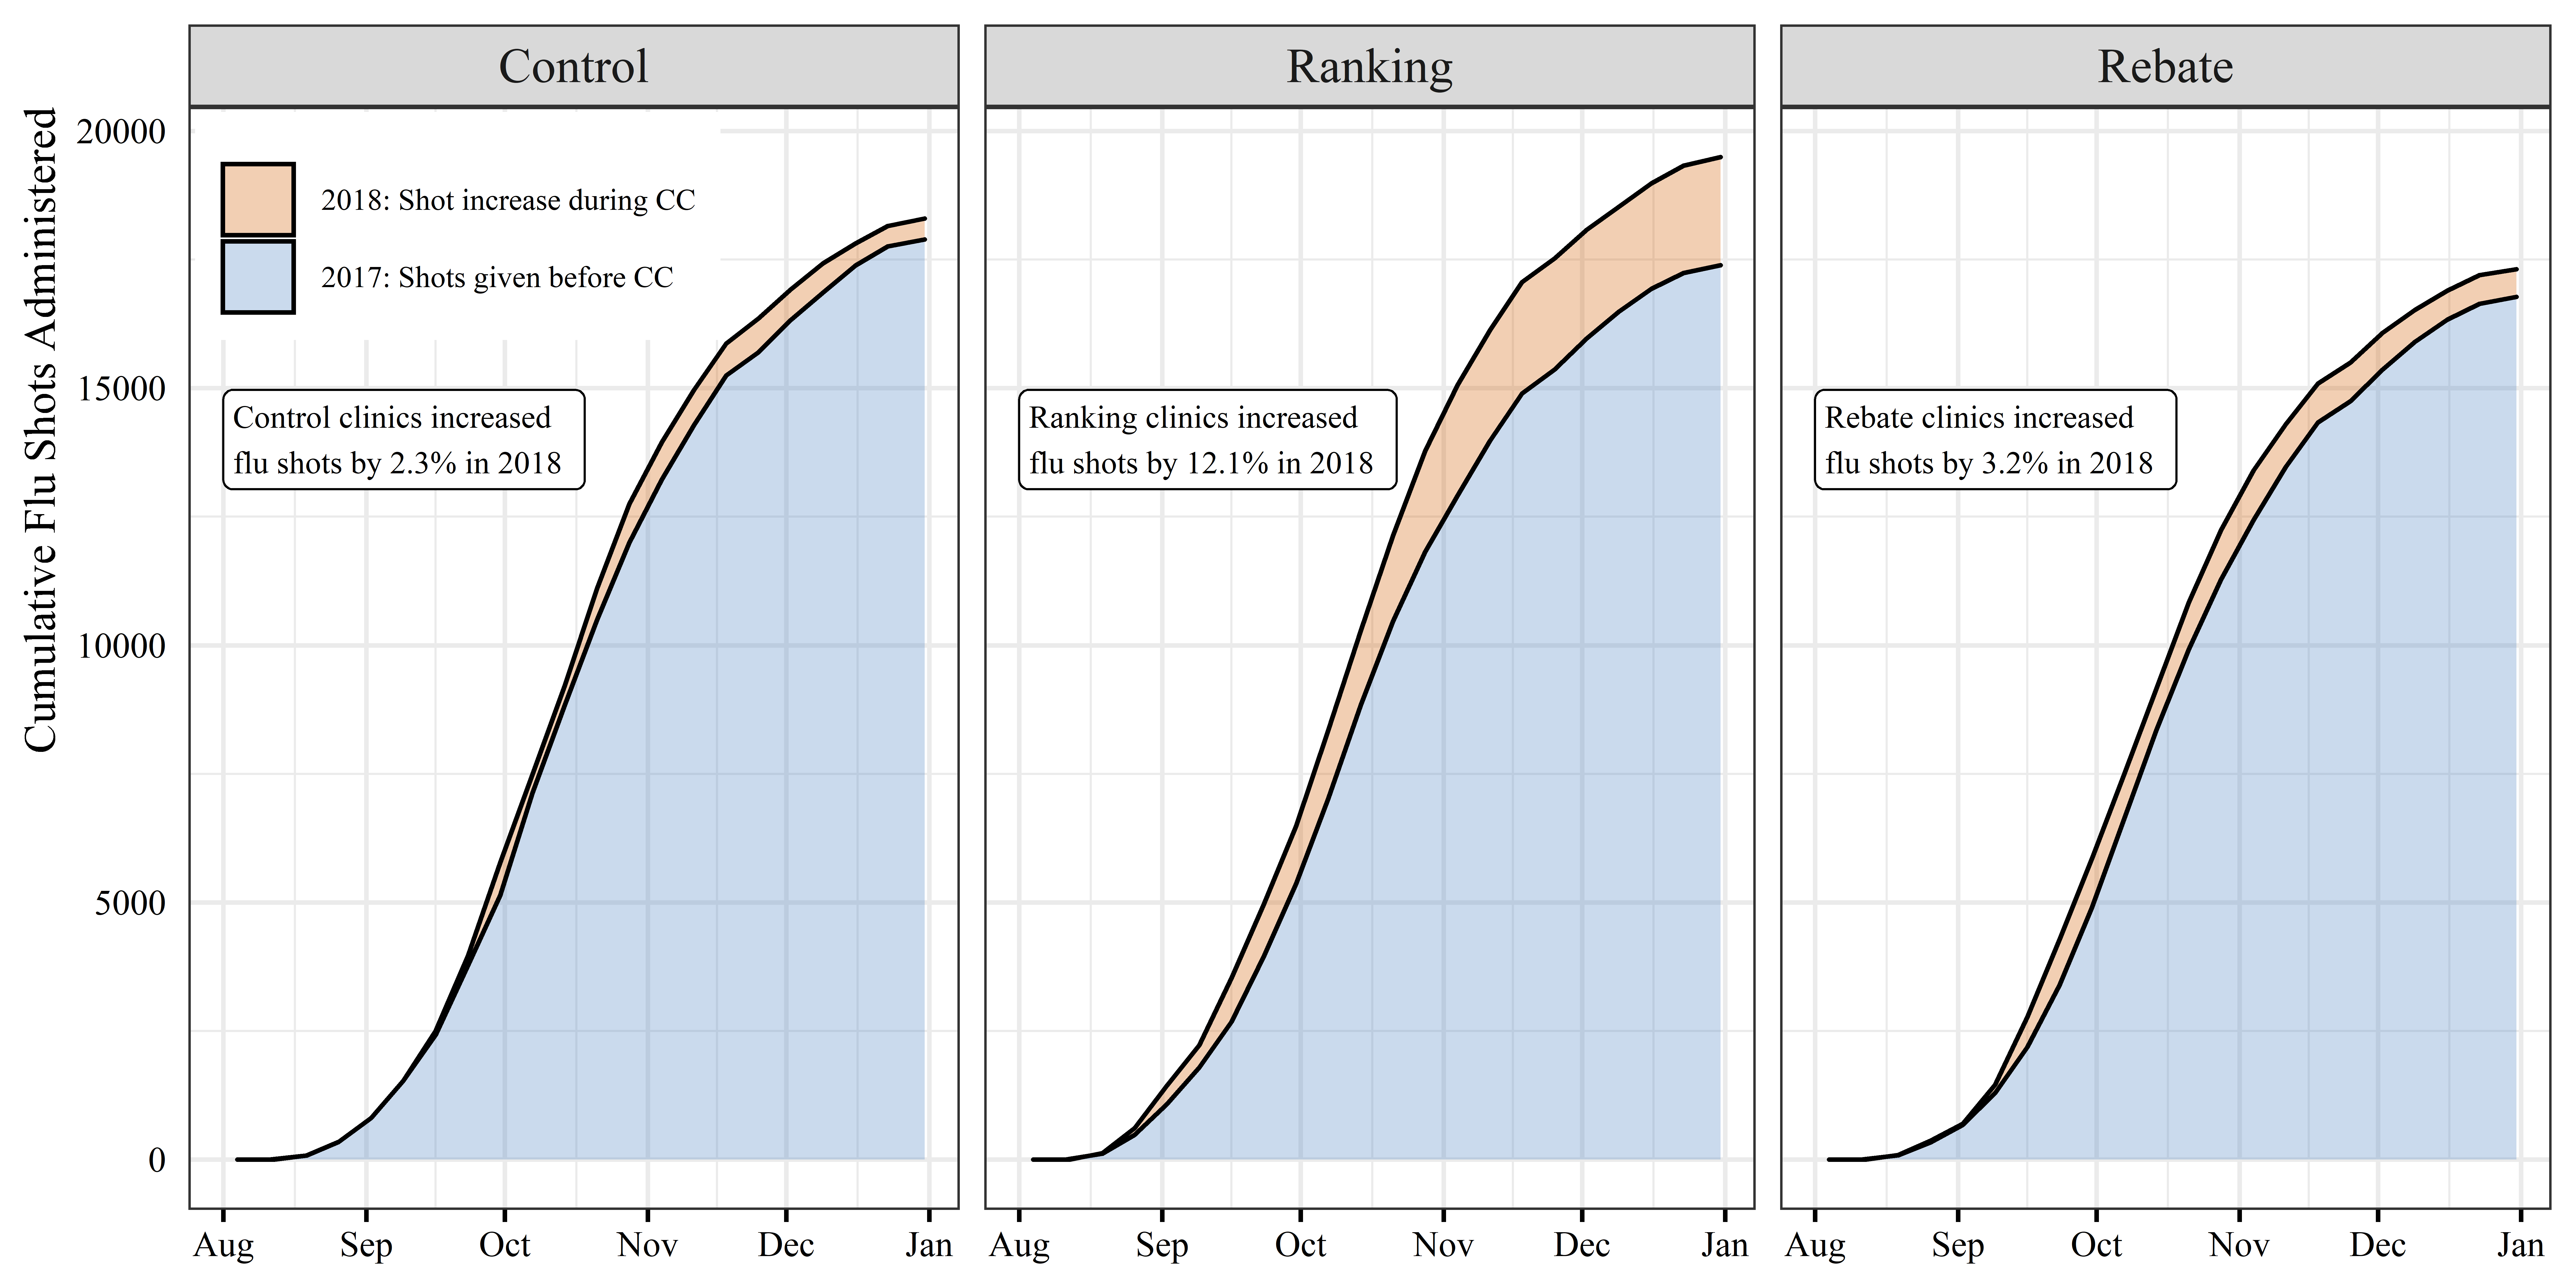
\includegraphics[scale=.75]{Figures/CC/CC_outcome_Fig1_color.png}     
     \label{fig:model_free_cc}
    %  \floatfoot{\textit{Note:} These are some figure notes... }
 \end{figure} 
 
 \subsection{Treatment Effect - Clinic Percent Growth}
 We first examine clinic flu shot percent growth during Compliance Care. For the statistical models that compare clinics from different groups, the most conservative approach is to exclude clinics without common support (N = 136, per Section 9). Taking the control as the base category, Table \ref{tab:teffect} reveals a statistically significant difference between the Ranking and Control clinics ($p < 0.05$). On average, the Ranking clinics grew their vaccines by 8.3\% more than the Control clinics while the Rebate clinics show no meaningful difference. Thus, we see support for Hypothesis 1b, but not Hypothesis 1a. These results carry through with an alternate dependent variable (Section 10). One other concern we address: Perhaps Compliance Care emails remind clinics to vaccinate – thus driving our effect. However, both the rebate and feedback conditions received emails, and as discussed next, a significant performance gap exists between the two. We proceed to compare the treated clinic outcomes.
 
  \begin{table}[htbp]
  \resizebox{.5\textwidth}{!}{ 
  \begin{threeparttable}[t]
   \centering
   \caption{Effect of Compliance Care on Clinic Flu Shot Percent Growth}
    \begin{tabular}{lc}
          & (1) \\
          & \textbf{Percent Growth} \\
          & \\
    Ranking (Post-Treatment) & 0.0833** \\
          & (0.0406) \\
    Rebate (Post-Treatment) & 0.00219 \\
          & (0.0399) \\
          & \\
    Observations & 2,720 \\
    \# clinics & 136 \\
    \end{tabular}%
    \medskip
    \begin{tablenotes}
      \footnotesize
      \item \textbf{Table Note:} Robust standard errors, clustered by clinic, in parentheses. Model also includes clinic patient count and clinic state fixed effects. 
      \item (*** $p < 0.01$, ** $p < 0.05$, + $p < 0.1$)
    \end{tablenotes}
  \label{tab:teffect}
  \end{threeparttable} }
 \end{table}
 
 \subsection{Comparison between Ranking and Rebate Groups}
 We expected the Rebate group to outperform all others. Instead, the results in Figure \ref{fig:model_free_cc} and Table \ref{tab:teffect} indicate that the Ranking group, who only received performance feedback, outperformed the Control and the incented Rebate group. To test for this, we performed Wald tests on the Table \ref{tab:teffect} coefficients to check whether (1) the Rebate clinics outperformed the Ranking clinics ($H_0: \beta_{1,rebate} >= \beta_{1,ranking}$) and whether (2) the Rebate clinics performed the same as the Ranking clinics ($H_0: \beta_{1,rebate} = \beta_{1,ranking}$). Both tests reject the null hypothesis ($p < 0.05$). Given the results of these tests, we conclude that the Rebate group did not outperform the Ranking group and instead the Ranking group outperformed the Rebate group by a statistically significant margin. Thus, we reject Hypothesis 2 in all cases. We next evaluate the effect of performance feedback within the Ranking clinics. 
 
 \subsection{Rank Response Behavior}
 During Compliance Care, VaxCare provided relative performance feedback to the clinics in the Ranking group. Each clinic identified at least one staff member to review and share this feedback with the rest of the clinic. As individuals within a firm coalesce around a common response, together they may alter the direction of the firm. Specification \ref{rank_resp} captures clinic response to their previous ranking (Table \ref{tab:rank_effect}, Column 1). 
 
 We observe statistically significant coefficients ($p < 0.01$) for both the linear and quadratic effect of the previous week’s rank. Figure \ref{fig:rank_resp} details the rank response function for each rank generated by these coefficients ($\lambda_1,\lambda_2$) after normalizing the average of these values to zero. This figure illustrates that being ranked last (Rank 46) in the previous week results in about a 2.5\% increase in shots per patient-population this week. In contrast, being ranked first correlates with a 0.8\% increase while being ranked twentieth correlates with a 1.0\% decrease in shots per patient-population. Even with clinic-level feedback, the response to being ranked near last strongly indicates the presence of Last-Place Aversion. We proceed to test the robustness of this finding.

  \begin{table}[p]
  \resizebox{.6\textwidth}{!}{ 
  \begin{threeparttable}[t]
   \centering
   \caption{The Effect of Rank on Weekly Shots per Patient-Population}
    \begin{tabular}{lcc}
          & (1)   & (2) \\
          & \textbf{WeekSPP} & \textbf{WeekSPP} \\
    Clinic Group & Ranking & Ranking \\
    Econometric Model & Specification 2 & Specification 3 \\
          &       &  \\
    Rank, previous week ($\lambda_1$) & -0.00209*** & - \\
          & (0.000648) & - \\
    Rank$^2$, previous week ($\lambda_2$) & 5.34e-05*** & - \\
          & (1.36e-05) & - \\
    Low Flag = 1 if Rank $\in$ & -     & [42,46] \\
    Coeff.: Low Rank ($\pi_1$) & -     & 0.0273*** \\
          & -     & (0.00767) \\
    High Flag = 1 if Rank $\in$ & -     & [1,5] \\
    Coeff.: High Rank ($\pi_2$) & -     & 0.00461 \\
          & -     & (0.00572) \\
          &       &  \\
    Observations & 792   & 792 \\
    \# clinics & 46    & 46 \\
    \end{tabular}%
    \medskip
    \begin{tablenotes}
      \footnotesize
      \item \textbf{Table Note:} Robust standard errors, clustered by clinic, in parentheses. Both models include week fixed effects for all Ranking clinics who started the vaccination season as VaxCare partners. The linear term in Specification 2 ($\lambda_1$) allows a clinic with a change in rank to either increase or decrease their effort, but not both. The quadratic term ($\lambda_2$) allows a change in rank to lead to an increase in effort for some ranks while allowing for a decrease in effort for other ranks. In Specification 3, we define last place as any of the bottom 5 ranks (42, 43, 44, 45, 46) and first place as any of the top 5 ranks (1, 2, 3, 4, 5). The Low Rank coefficient shows that moving into the bottom ranks leads to a +2.73\% change in shots per patient-population the following week. 
      \item (*** $p < 0.01$, ** $p < 0.05$, + $p < 0.1$)
    \end{tablenotes}
  \label{tab:rank_effect}
  \end{threeparttable} }
 \end{table}

 \begin{figure}[p]
     \centering
     \caption{Rank Response Function} %\medskip
     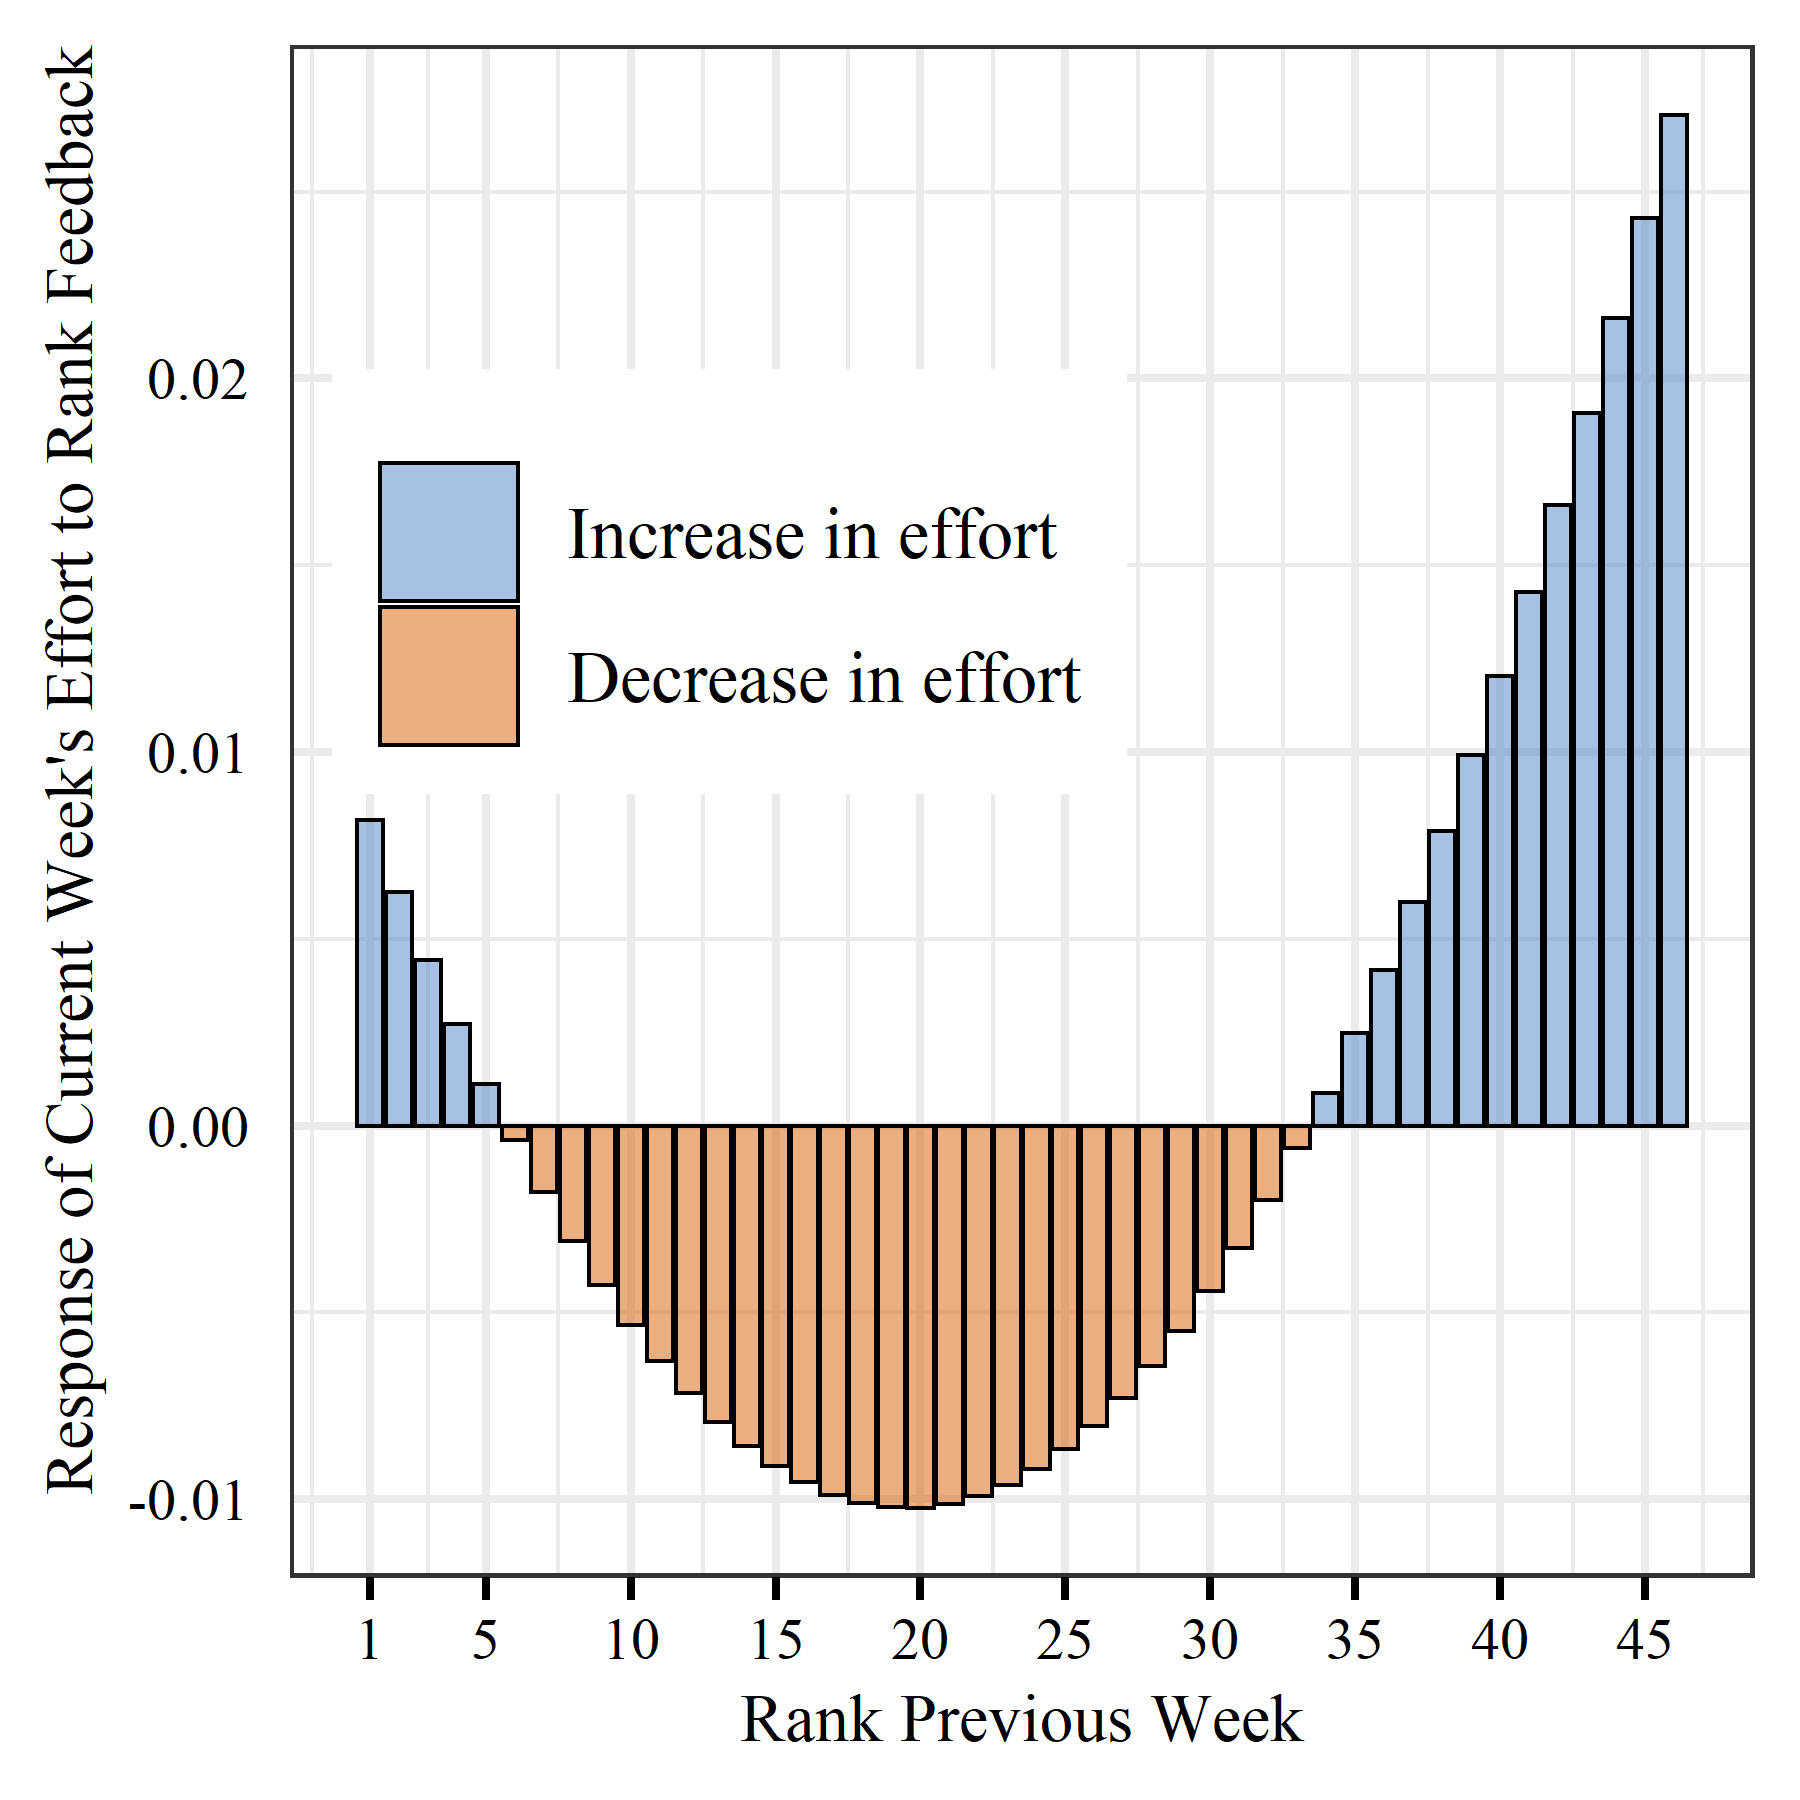
\includegraphics[scale=1]{Figures/CC/Rank Response - Ranking Group (color).png}     
     \label{fig:rank_resp}
    %  \floatfoot{\textit{Note:} These are some figure notes... }
 \end{figure} 
 
 \subsubsection{Rank Response: Definitions of First and Last Place}
 Given our clinic context, how should we define “first” or “last” place? We initially define “first place” as the top 5 ranks and define “last place” as the bottom 5 ranks to match; we then vary these definitions and test the sensitivity of our findings. More than 20\% of the clinics rotate through the bottom 5 ranks, and only 4 clinics spend a majority of the vaccination season there. On the other hand, almost 40\% of the clinics move through the top 5 ranks but only a handful of clinics spend a majority of the vaccination season in the top 5. To further clarify the presence of FPL and LPA, we evaluate the following model using a Fixed-Effects framework. The \textbf{HighRank} and \textbf{LowRank} indicators are set to 1 if the clinic receives a ranking in the top 5 or in the bottom 5 (respectively), and 0 otherwise.

 \begin{equation} \label{rank_resp_ind} %\begin{split} %\end{split} 
       WeekSPP_{it} = \pi_0 + \pi_1 \mathbbm{1}\{LowRank\}_{i,t-1} + \pi_2 \mathbbm{1}\{HighRank\}_{i,t-1} + Week_t + Clinic_i + \epsilon_{it}
 \end{equation}  
 
 We find that moving into these positions is followed by an increase in shots per patient-population by week (Table \ref{tab:rank_effect}, Column 2). A clinic which receives a low rank leads to a +2.73\% change in shots per patient-population the following week ($p < 0.01$), but a clinic given a high rank does not yield a statistically significant change ($p > 0.15$). A formal test rejects ($p < 0.05$) the null hypothesis that receiving a low rank has the same effect as receiving a high rank ($H_0: \pi_1 = \pi_2$). These results hold under various definitions of first and last place (Section 11): We observe LPA – but not FPL behavior – under a wide range of definitions. 
 
 \subsubsection{Rank Response: Robustness} \label{rpf_robust}
 Given our econometric setup, we must rule out “mean reversion” as an alternative explanation for our results. Poor performance weeks could follow high performance weeks (and vice versa), either because of fluctuation in demand or a provider’s attempt to “catch up.” If this behavior coincided with changes in rank, our explanatory variables could pick up this reversion. To test for this, we artificially ranked the clinics in the Control group (with respect to each other) and the clinics in the Rebate group. We then tested for rank response behavior in these clinics, similar to a “placebo” test, since neither of these groups actually received performance feedback. A subset of these results can be seen in Table \ref{tab:rank_art} with a complete discussion in the Appendix (Section 12). We do not see any evidence of LPA in either the Rebate or Control groups. In the end, Last-Place Aversion as we define here manifests only among the Ranking clinics, affirming our approach and eliminating the possibility of mean reversion driving our results.
 
 We also explore whether LPA degrades with time. We find the effect intensifies with time. By adding a count of the number of weeks spent near last to Specification \ref{rank_resp}, we find the effect of one extra week ranked in the bottom 5 is statistically significant ($p < 0.01$) and is approximately the same as being ranked “35 out of 46.” We also observe stronger responses to ranking information later in the vaccination season.
 
 In conclusion, we find strong evidence to support Hypothesis 4 (Last-Place Aversion) but do not find enough evidence to support Hypothesis 3 (First-Place Loving behavior). 
 
 \begin{table}
  \resizebox{.85\textwidth}{!}{ 
  \begin{threeparttable}[t]
   \centering
   \caption{Clinic Response to “Artificial” Ranks for Rebate and Control Groups}
    \begin{tabular}{lcccc}
          & (1)   & (2)   & (3)   & (4) \\
          & \textbf{WeekSPP} & \textbf{WeekSPP} & \textbf{WeekSPP} & \textbf{WeekSPP} \\
    Clinic Group & Rebate & Rebate & Control & Control \\
    Econometric Model & Specification 2 & Specification 3 & Specification 2 & Specification 3 \\
          &       &       &       &  \\
    Rank, previous week ($\lambda_1$) & 0.000867 & -     & -0.000163 & - \\
          & (0.000782) & -     & (0.000940) & - \\
    Rank$^2$, previous week ($\lambda_2$) & -1.83e-05 & -     & -4.98e-06 & - \\
          & (2.10e-05) & -     & (2.66e-05) & - \\
    Low Flag = 1 if Rank $\in$ & -     & [44,48] & -     & [42,46] \\
    Coeff.: Low Rank ($\pi_1$) & -     & -0.0121 & -     & -0.0193 \\
          & -     & (0.0164) & -     & (0.0187) \\
          &       &       &       &  \\
    Observations & 823   & 823   & 742   & 742 \\
    \# clinics & 48    & 48    & 46    & 46 \\
    \end{tabular}%
    \medskip
    \begin{tablenotes}
      \footnotesize
      \item \textbf{Table Note:} Clinic-robust standard errors in parentheses. All models include week fixed effects. 
      \item (*** $p < 0.01$, ** $p < 0.05$, + $p < 0.1$)
    \end{tablenotes}
  \label{tab:rank_art}
  \end{threeparttable} }
 \end{table}
 
 \subsection{Overall Implications of Relative Performance Feedback}
 Compliance Care 2018 led to an increase in flu shots, particularly for the group given RPF. As the season progressed, clinics might have competed for higher ranks or simply tried to avoid falling behind. But which clinics improved? Are the high performers “over-achieving”? Or have we pulled up the performance of the clinics who would generally have watched the season progress without extra effort?
 
 To answer this question, we use the artificial rankings for the Control clinics (Section \ref{rpf_robust}) to match these clinics to the Ranking clinics at the end of the season. These matched Control clinics serve as a counter-factual for the Ranking clinics had they not received RPF. Please see Figure \ref{fig:rank_v_ctrl} for reference, where higher ranks (i.e., 42-46) signify worse performance and lower ranks signify better performance. With only two exceptions, the Ranking clinics outperform their similarly ranked Control clinics. Overall, the Ranking clinics outperform their respective controls by 10.3 percentage points. The great gap emerges among the clinics with negative performance (administered fewer shots in 2018), where the Ranking clinics outperform their respective controls by 22.9 percentage points (Figure \ref{fig:rank_v_ctrl}, top left quadrant).  
 
 Thus, while relative performance feedback elevated the performance of nearly all Ranking clinics, this is particularly true for the worst performing clinics. Last-Place Aversion appears to have enticed poor performing clinics to continue to vaccinate and “stick with the program.” These results are consistent with the literature on general performance feedback \citep[e.g.,][]{Kuhnen2012,Charness2014} while also illustrating how improvement may vary depending on the specific rank or place \citep{Gill2019}. Although our rankings are anonymous, our result is similar to \cite{Song2018a} in that the poor performers gain the most from RPF. We further link this reaction to an aversion for being ranked near last, similar to \cite[p. 35]{Buell2021}: “…that the desires to get out of and to avoid falling into last place, are powerful motivators that can help drive human behavior.” We find exactly that: An aversion for last (even generally defined) drives beneficial behavior and performance improvement.
 
 \begin{figure}[htbp]
     \centering
     \caption{Performance Gap between Ranking and Control Clinics by Rank at End of Experiment} %\medskip
     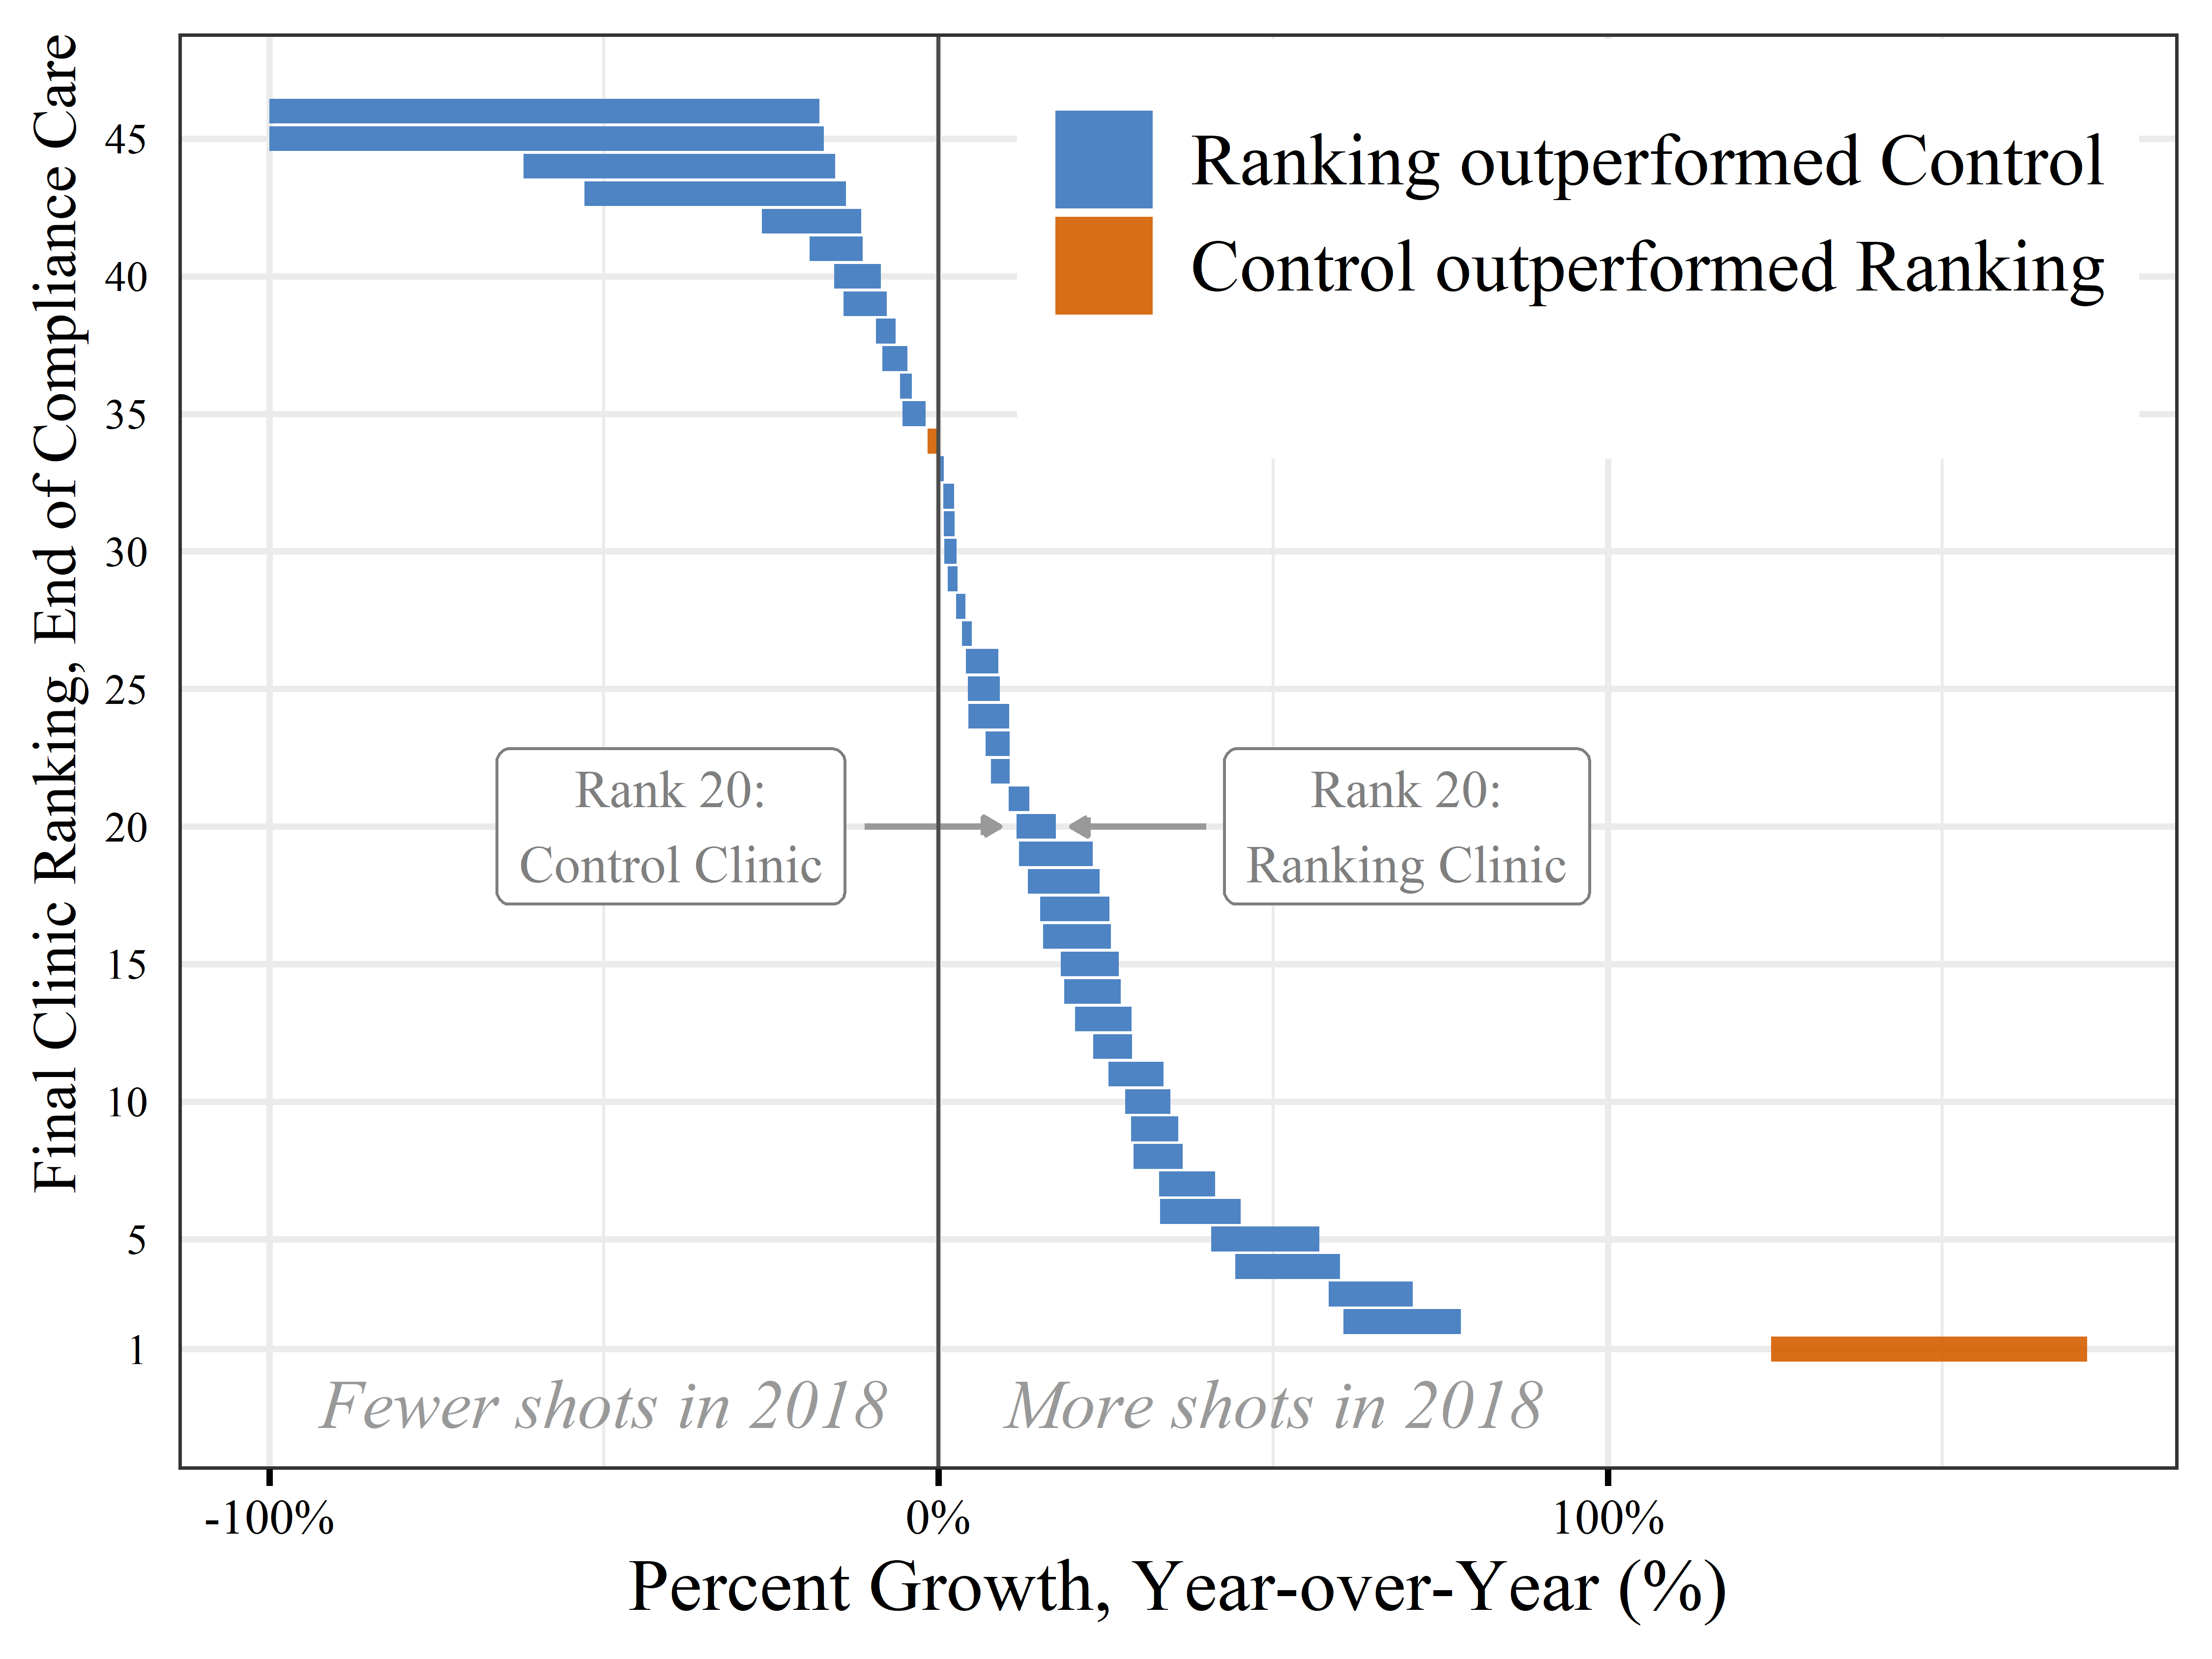
\includegraphics[scale=1]{Figures/CC/CC_RankVsControl_Fig3_color.png}     
     \label{fig:rank_v_ctrl}
     \floatfoot{\textbf{Figure Note:} This figure illustrates the clinic-to-clinic performance gap between hypothetically ranked Control clinics and the Ranking clinics at the end of Compliance Care. Larger bars indicate greater gaps. Darker shaded bars indicate ranks where the Ranking clinics outperformed Control clinics.}
 \end{figure} 


\section{Discussion \& Conclusion} \label{Conclusion_CC}
 The CDC continues to look for ways to achieve broad-scale compliance with recommended vaccination protocols, and for good reason. During the 2018-19 flu season, the CDC estimates the flu vaccine averted up to 7.1 million instances of flu-like illness and 3.8 million medical visits \citep{Chung2020}. Compliance starts with public interest: Consider that there were 4-times the number of Google searches for “flu vaccine” in August 2020 than a year prior as concerns of a Covid-19 and influenza “twindemic” escalated \citep{Google2021,NYTimes2020}. Even so, the lack of recent flu shot progress reveals a rift between vaccine interest and vaccine compliance, yielding critical implications for reducing the effects of influenza as well as the deployment of other vaccines going forward.
 
 The inherent nature of flu vaccine compliance complicates any solution since compliance requires action by two parties: Providers and patients -– the supply- and demand-side of the equation. Despite individual successes increasing demand \citep[e.g.,][]{Milkman2011}, the flu vaccination rate remains largely unchanged. But studies find most patients would accept the vaccine if their provider simply recommended it \citep{Patel2017}. And since patients still report their primary care provider as the most frequent flu vaccination channel \citep[48\%, per][]{CVSHealth2018}, we believe the greatest opportunity for large scale improvement lies in vaccine provision by providers rather than vaccine solicitation from providers. 
 
 Given this approach, Compliance Care successfully encouraged treated clinics to administer more flu shots. The program led to a 5.5 percentage point increase in flu shots for the treated over the control clinics. Clinic improvement is asymmetric, though: The Ranking clinics outperformed the Control clinics by 9.8 percentage points, while the Rebate clinics only outperformed the Control clinics by 0.9 percentage points. We claim that Last-Place Aversion meaningfully drives this outcome: Despite their low ranking, the gap between the Ranking and Control clinics widened over the season such that, in the end, the worst performing Ranking clinics outperformed their respective Control clinics by 22.9 percentage points. Our supply-side approach: (1) cued attention to flu shots with (2) a near-costless intervention while still (3) preserving provider discretion by intervening at the clinic-level. Our results hold promise for addressing the broader flu vaccination problem in an effective and cost-considerate manner.
 
 Our paper makes several contributions to the literature. First, we highlight the motivational power of social comparison \citep{Festinger1954}, even over and above economic incentives. In our context, performance feedback dominates the effect of additional financial incentives. However, our experiment is limited in that we only compare one form of financial incentive to one form of RPF. To explore this, we worked with VaxCare to distribute a survey to clinics after the study ended. Among the rebate clinic respondents, 75\% indicated the incentive amount was meaningful – so we do not believe the size of the incentive was driving our result. Future work could compare different incentive systems and even explore a combination of incentives and feedback. Even so, our counter-intuitive result highlights an opportunity to leverage low-cost interventions to effectively focus healthcare provider attention on an issue of interest. 
 
 Second, when considering the clinic rankings and the role of RPF, we also find evidence of Last-Place Aversion, similar to \cite{Kuziemko2014,Gill2019} and \cite{Buell2021}. To the best of our knowledge, our analysis is the first to examine rank response behaviors in productivity among firms in a dynamic, real-world setting. Specifically, Last-Place Aversion manifests not only in individuals, but also among firms. Furthermore, the strongest effect appears among the worst performing Ranking clinics. 

 This finding comes with one limitation: Our field experiment and subsequent identification of a response does not permit us to identify the mechanism behind the response. We have demonstrated the efficacy of financial incentives and performance feedback, but some of the reasons underlying the outcomes remain untested. These reasons include exploring what specific behavior the incentive did not affect or why a clinic exhibits Last-Place Aversion or whether these behavioral changes might persist over time. Other possible mechanisms include clinics fearing repercussions of low rankings or providers perceiving the clinics as reaping the financial benefits of their individual effort. Future work should seek to clarify the processes of behavior change as well as exploring the time-sensitive nature of these behaviors (e.g., “Does Last-Place Aversion diminish over time?”). 

 Third, we contribute to the growing body of work in operations that finds an important role for discretion in driving operational performance \citep[e.g.,][]{VanDonselaar2010,Campbell2011,Kim2015,Phillips2015,Ibanez2017,Song2018a}. Vaccination rate information given to clinics then successfully diffused to front-line workers. Thus, performance feedback, even when given at a higher, firm-level, encouraged the productive use of individual discretion to improve operational performance. Few studies examine firm-level response to feedback and incentives; even fewer compare the two. Our approach fills both gaps by cueing provider attention to administer more flu shots.

 This approach raises two follow-on thoughts. First, the focusing of attention on flu shots inherently begs the question of where providers are paying less attention as a result. We are limited from seeing how other elements of patient health were affected. Despite this, because we intervene at the clinic level, we mitigate the concerns of “alert-fatigue,” which has already been shown to negatively impact patient outcomes. Instead, we allow providers full discretion in their final choice of patient care and we trust these individuals to make the best decisions for their patients. Second, given our findings, one might hypothesize about the benefits of a dual supply- and demand-side approach to vaccination compliance, as in \cite{Zimmerman2014}. Indeed, our findings clarify which elements of these more complicated approaches meaningfully alter vaccination outcomes. Future research should build on our work by combining effective supply-side cues with proven demand-side strategies, such as patient reminders.

 Finally, as a general contribution, we demonstrate the importance of running field experiments when addressing complicated operational questions \citep{Ibanez2019a}. Field experiments possess explanatory power and identification advantages which can augment archival data methods to generate both rigorous and relevant research. Given our experimental design, our results will likely generalize to other contexts: Consider that the above behaviors manifest in a randomized setting with many independent, geographically dispersed clinics despite heterogeneity in location, clinic size, and performance. Even so, we acknowledge that the clinics in this study represent VaxCare partners that consented to join the experiment. Future work should continue to study these topics in other industries and explore whether incentives or performance feedback lead to differing rates of intervention attrition.
 
 One limitation exists surrounding our experimental design. After recruitment, no further action was taken with the Control group; this setup most accurately replicates the real-world setting for a VaxCare partner. Because of this, the possibility remains for an email “reminder” effect for the treated clinics. This effect seems unlikely – as the Rebate clinics receive emails and still do not statistically outperform the Control clinics – but we recognize the inherent limitation of our clinical context. 
 
 Our findings have a number of managerial implications. First, although many organizational interventions lead to performance improvement, Compliance Care achieved improvement in a domain bereft of significant improvement in more than a decade with minimal cost. As mentioned before, even a 1 percentage point increase in vaccine coverage could yield significant societal benefits. If half of these shots went to seniors – a higher risk age group – CDC reports estimate this would prevent more than 2500 hospitalizations \citep{Rolfes2019}. Furthermore, the effects of RPF are “long-lasting” \citep{Blanes-i-Vidal2011} and persistent \citep{Delfgaauw2013}. Thus, we expect enduring benefits from any positive outcome, even under financial constraints. Furthermore, policy makers can leverage other operations literature to scale our intervention \citep{Drakopoulos2017, Gupta2020}.
 
 Second, we note that operational structure helps to selectively focus decision makers’ attention. Small attention cues can encourage decision makers in any organizational context to selectively focus their attention on important tasks \citep[e.g.,][]{Song2018a,Kim2020}. Finally, we must note that one cannot cue attention to all desired behaviors. The introduction of multiple cues would likely reduce the effectiveness of each cue with a potentially worse end state. We caution managers to be mindful of their use and to prioritize interventions which achieve the greatest benefit via the smallest impact.
 
 We conclude appropriate supply-side behavioral intervention programs can improve performance, even when targeting seemingly immutable trends, such as influenza vaccination rates. Our results show promise for improvements in public health and more generally for company operations.
 

\end{onehalfspace}

\section*{Acknowledgements}
We thank management at our research site for their cooperation. We thank Charles Corbett, the AE, and reviewers for helpful comments that have improved the paper. Any mistakes remain our own.  

\bibliographystyle{apacite}
\bibliography{Bibliography/bib_ComplianceCare_3feb22}




% Chapter 2


% Chapter 3
\chapter{The Value Behind Traffic: How Patient Discretion and Information Coarseness Altered Healthcare Traffic in the Wake of COVID-19}

\section{Introduction}
 Many aspects of company operations depend on understanding customer traffic \citep{Gallino2014}. \cite{Perdikaki2012} argue retailer profitability directly depends on the ability to track traffic, for several reasons. First, traffic informs labor planning \citep{Mani2015,Chuang2015,Perdikaki2017,Netessine2010}. Second, variation in traffic can highlight operational problems in other areas \citep{Lee2017}. And finally, understanding traffic patterns enables better traffic prediction \citep{Yung2020,Kamalahmadi2021,Abrishami2018}. Traffic represents a key operational input -- especially in healthcare. Even with growing acceptance of telemedicine \citep{WSJ_21_telemed,Friedman2021}, limits remain: For example, a physician cannot perform a physical or administer vaccines without seeing patients in-person. Many aspects of healthcare cannot happen from a distance \citep{Romanick-Schmiedl2020}, and serious consequences follow delayed or omitted care \citep{Findling2020,CDC_ExcessDeath}. Operational success depends on tracking traffic, but it was not until March of 2020 that the dependence became brutally obvious.
 
 With the emergence of the SARS-CoV-2 virus and the associated disease (Covid-19), traffic to many clinics vanished overnight. Some preventive care measures dropped by more than 80\% \citep{Cantor2020}. The declines were so precipitous and so concerning, a campaign in July 2020 advised: “Stay 6 feet away from others, stay close with your doctor" \citep{StopMedicalDistancing.org}. Such drops possess grave implications for patient welfare \citep{WSJ_skipDoc}, and so we ask: “What factors drove healthcare clinic traffic during the Covid-19 pandemic?" Our work empowers clinics to better meet patient needs \citep[as in][]{Musalem2020} and accurately predict traffic moving forward. 
%  perhaps as much as 50\% of the US population delayed some type of care in 2020 \citep{Findling2020}.

 To date, as evidenced by the plethora of studies listed in \cite{Gupta2020}, the state-wide “stay-at-home" or “shelter-in-place" orders remain the literature's primary concern. But stay-at-home orders cannot fully explain the drop in clinic traffic. Many states issued orders, but most clinics remained open through exemptions for “essential services." Moreover, individual decisions and personal preferences appear to drive willingness to engage with in-person activities more than the state-wide orders \citep{Goolsbee2020_key}. Figure \ref{fig:t2_mot_fig} affirms this insight using observations from our study: \textit{Personal mobility} (i.e., Trips per Person), which captures a willingness to travel, drops even before stay-at-home orders go into effect. And so our paradigm evolves: To improve patient health, you must see them in-person. To see them in-person, you have to be open. But just being open cannot suffice: They must also decide that they want to be seen.
 
 \begin{figure}[!b]
    \centering
    \caption{Trips per Person, or personal mobility, drops before shutdown orders go into effect. The drop also coincides with an increase in search engine interest in Covid-19.}
    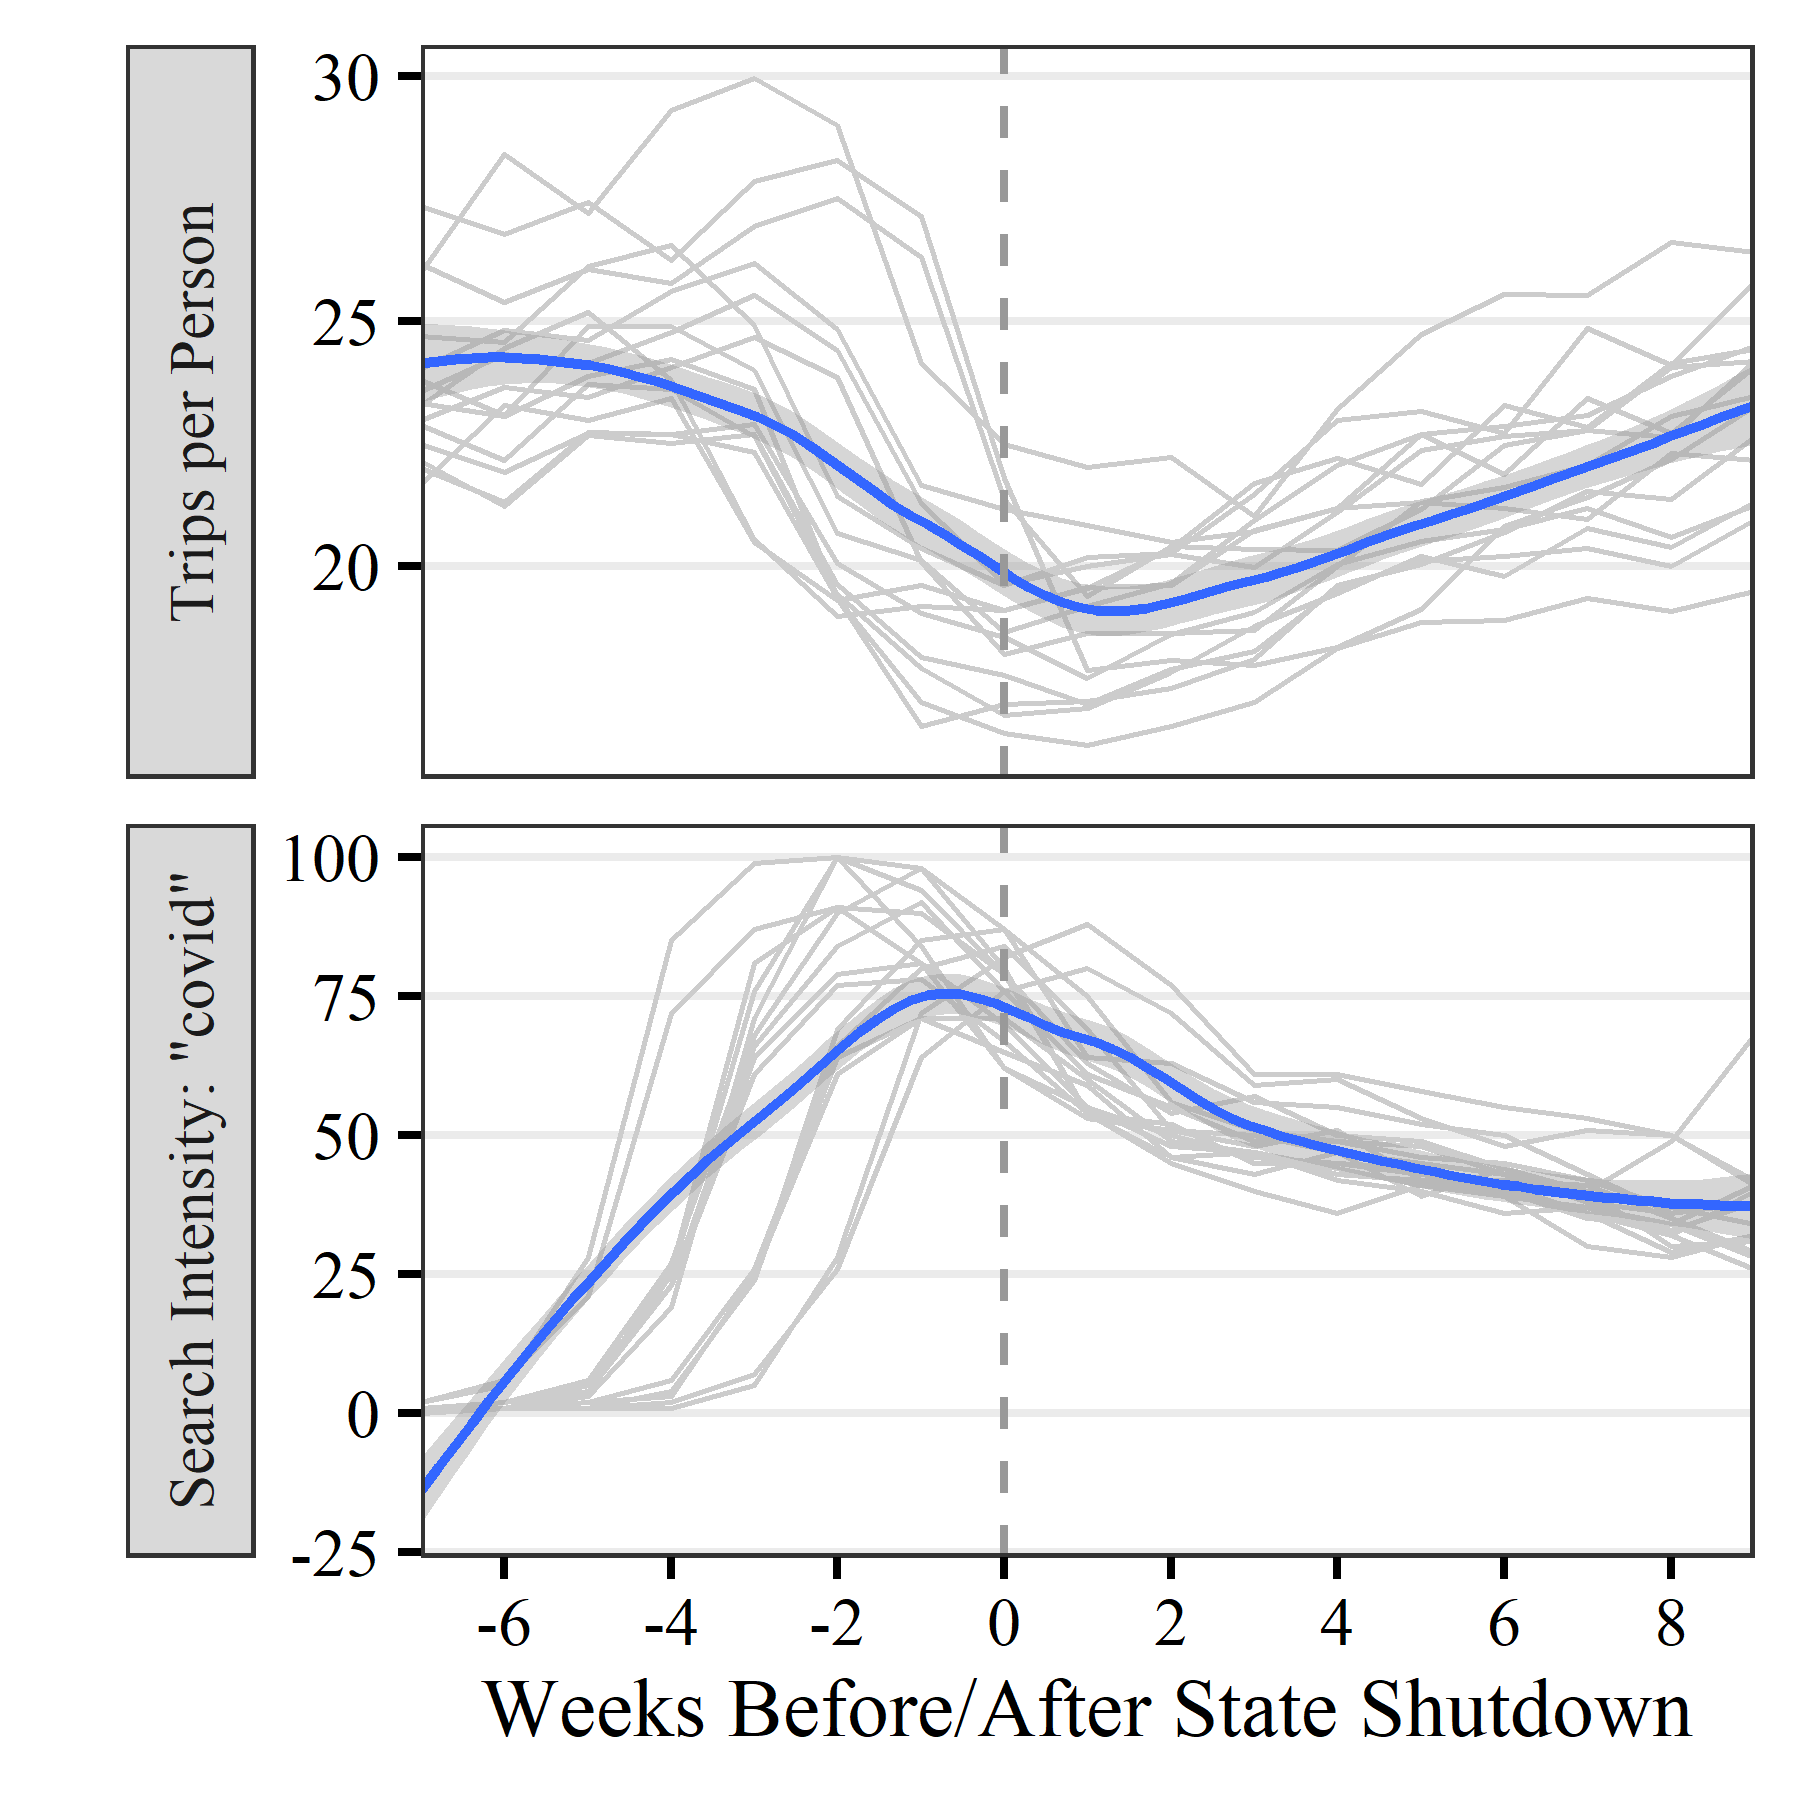
\includegraphics[scale=1]{Figures/VC2/MotFig-Take2.png}     
    \label{fig:t2_mot_fig}
    \floatfoot{\textbf{Figure Note:} The figure plots mobility and search data for 15 US states relative to the stay-at-home order for each state. The 15 states represent the states for which we also have clinic traffic observations (Section \ref{data}). The blue line depicts a “Loess" conditional smoothing function applied to the raw data. The graph illustrates “Trips per Person" as recorded by the \cite{MTI2020}. “Search Intensity" represents user searches for the word “covid" from \cite{Google2021}, where intensity varies from very few to many searches on a scale from 0 to 100. }
 \end{figure}  
 
 What then influences the decision to be seen? Executive orders might influence some behavior, but patient discretion and personal preferences ultimately dictate mobility today, and tomorrow, and beyond. In contrast to such orders, Figure \ref{fig:t2_mot_fig} shows a drop in mobility coincides with an increase in Google search intensity. Perhaps mobility drops with greater fear of Covid \citep{Alfaro2020}, but then what drives such fear? Signals of environmental safety could incite fear, either as a coarse mandate (e.g., “Stay home: It is not safe to go out") or a precise nudge (e.g., “10\% of people in your area are sick"). But for every push, see a pull: Fear compels someone to stay home, and \textit{value} invites someone to go out. If we allow discretion in movement -- that is, if we allow a patient to choose between staying or going -- we must then consider the value generated by such movement.
 
 In studying movement value, traffic cannot simply remain an overarching construct, as high-value trips might pull patients more. If mobility drops but remains non-zero (see Figure \ref{fig:t2_mot_fig}), then trips that remain must generate greater value than trips that fade. Hence, we ask: “During the pandemic, how does the value of the service consumed impact healthcare clinic traffic?" We operationalize the question by comparing general trips to a clinic (less valuable) to trips which specifically include vaccination (more valuable). Clinic “traffic" nests both, and both serve important roles in patient health. But delaying or omitting vaccinations poses immediate risks to the patient and the community \citep{Salmon2015,Brewer2017}; the flu vaccine alone averts tens of thousands of hospitalizations each year \citep{CDC2020}. And so we examine the pull of different services and discuss the implications for clinic traffic predictions. 
  % Cite Brewer? Phadke?

 Our approach also models the push to stay home because of signal coarseness. Coarse signals about Covid-19 might be easier to understand while precise signals might be easier to use \citep{Morris2007}. Executive, state-wide stay-at-home orders represent coarse signals of environmental safety while local, publicly available Covid metrics (e.g., case counts) represent precise signals. To answer our research questions, our study combines observations from: Healthcare clinics across 15 US states; anonymized county-level cell phone mobility observations; county-level Covid-19 measures; and public information on state-wide stay-at-home orders. During our study period, three factors interact to shape healthcare clinic traffic: (i) Individual mobility preferences, (ii) the value of the care sought, and (iii) the perception of disease severity.
 % We also explore whether the severity of the precise signals matters by comparing changes in the effect of mobility with signals of lower severity (Covid case counts) and signals of higher severity (Covid death rates).
 
 Based on our empirical analysis, we find the following. \textbf{First}, clinic traffic returns with rising personal mobility. The size of such returns, however, vary significantly: A 1\% increase in mobility yields a large return to vaccination traffic (+2.169\%) but a fractional return to non-vaccination traffic (+0.56\%). More mobility means more traffic, depending on the type of care and value provided, one contribution of our study. \textbf{Second}, precise signals dominate coarse signals in affecting non-vaccination traffic. Precise signals also attenuate the effect of mobility on such traffic, especially when signaling even greater hazard (e.g., rising Covid death rates). In choosing information coarseness, trade-offs abound in the literature. We contribute to the debate by comparing one coarse signal, which has no impact, to precise signals which alter both mobility decisions and clinic outcomes. \textbf{Finally}, aside from personal mobility, no other factors have any detectable impact on vaccination traffic. Priorities emerged as states started reopening and people decided to leave home, revealing people may consider vaccinations more important than other elements of primary care. By studying the effect of such decisions, we identify and characterize powerful predictors of healthcare clinic traffic.

 In executing our study, we also add to emerging literature exploring effects of the Covid-19 pandemic. As surveyed in \cite{Gupta2020a}, most studies focus on the implications of stay-at-home orders; many examples exist in economics \citep[e.g.,][]{Goolsbee2020_key,Goolsbee2020_unpub,Alfaro2020,Cantor2020,Alfaro2021,Ziedan2020,Farboodi2020,Zhang2020}, though we know of only one published example in operations \citep{Wang2021}. As discussed in \cite{Wang2021}, such studies generally focus on mobility as the outcome of interest (p. 4). In contrast, our study considers mobility the aggregated decisions of individuals which then act as an input and predictor for our outcome, clinic traffic. To the best of our knowledge, no other studies have used personal mobility to predict changes in traffic during the pandemic. We also contribute by leveraging developments in machine learning to enhance our identification strategy.
 
 In Section \ref{HD_VC2}, we position our study in the broader literature which we use to develop and motivate our hypotheses. Section \ref{Empirical} describes our data and our empirical strategy. Section \ref{Results_VC2} presents our results and a post-hoc analysis. Section \ref{Conclusion_VC2} concludes.
 

\section{Hypothesis Development} \label{HD_VC2}
\subsection{Mobilizing Differently: The Effect of Value}
 In operations, traffic represents a critical input for many system-level outcomes \citep[e.g.,][]{Perdikaki2012}. Without an adequate understanding of traffic, other operational efforts may yield no benefit, including efforts like inventory management or queue design. For example, traffic informs labor planning \citep[e.g.,][]{Chuang2015} and inadequate labor planning can lead to poor service and employee attrition \citep{Ton2008}. \cite{Lee2017} illustrate a retail situation where high traffic and insufficient staffing lead to “phantom stockouts" because inventory is shelved incorrectly. And low traffic to clinics \cite[such as documented by][]{Mehrotra2020,Mehrotra2021} erodes clinic revenue and limits the ability of providers to monitor chronic conditions. In sum: Unanticipated traffic in either direction complicates operational planning.
 
 Even so, individual willingness (or reluctance) to travel precedes clinic traffic; we refer to such willingness as “personal mobility." While some studies explore how mobility affects other factors \citep[e.g., the spread of infection in][]{Dave2020}, the emerging literature in economics mostly focuses on how the stay-at-home orders orders affect mobility \citep[review in][]{Gupta2020}. And yet \cite{Goolsbee2020_key} argue individual reluctance to venture out dominates the effect of the stay-at-home orders. Similar implications emerge for preventative, elective, and outpatient traffic \citep{Ziedan2020,Cantor2020}, but such studies lack a coherent reason for why patients delayed some elements of care but not others \citep{Czeisler2020}. Factors beyond just state-wide stay-at-home orders might explain variance in clinic traffic better.
%  Cite Dave2021?
 
 We propose the value of the care informs personal mobility which then drives clinic traffic. One case in point: Early in the pandemic the American Medical Association issued guidelines to help private practices “triage" different types of care \citep{AmericanMedicalAssociation2020}. The guidelines included assessing patient risk and treatment urgency, two inputs to the value of care. To operationalize value, we classify non-vaccination traffic as less valuable and vaccination traffic as more valuable; we then study how personal mobility decisions affect the two types of traffic. Patients delayed or omitted less valuable care at record levels during 2020 \citep{WSJ_pcp,WSJ_skipDoc}, while the medical community claims “... vaccination is one of public health’s greatest achievements" \citep[p. 190]{Brewer2017}. In fact, industries such as healthcare and education commonly require vaccination records for employees and patrons \citep{CDC_stateVaccReq}. Given such differences and conditional on a willingness to leave home, we propose more valuable care will return faster than less valuable care with increasing mobility.
%  even emergency departments saw drastic reductions in care \citep{Hartnett2020}.

 \medskip \noindent
 \begin{tabularx}{\linewidth}{ r X }
    \textbf{Hypothesis 1:} & \textit{An increase in personal mobility will correspond to \underline{greater} returns to more valuable care (vaccination traffic) than to less valuable care (non-vaccination traffic).} [H1]
 \end{tabularx}   %\medskip

\subsection{Mobilizing Safely: The Effect of Signaling}
 Next, we explore the effect of different types of public information on clinic traffic. In philosophy and economics, studying the “social value of public information" or signals extend back decades \citep[p. 1]{Morris2002}. \cite{Lewis1969} argues that signaling conventions yield what \cite{Grice1957} calls “meaning," where common knowledge of a signal's intention represents a key element of conventions. Said differently: Common knowledge begets conventions. Conventions reveal the intentions of a signaler and facilitate shared understanding. And “[successful] communication rests on shared understanding" \citep[p. 594]{Morris2007}.
 
 Pursuing shared understanding, however, might compromise signal precision through an increase in information \textit{coarseness} \citep{Morris2007}. For example, assigning a coarse grade of “Pass" instead of a precise “73/100" might yield broader comprehension \citep{Harbaugh2018}. In such a decision, trade-offs abound: Coarse information is easier to process \citep{Harbaugh2018} and increases the likelihood of “shared understanding," but “unsophistication" and imprecision can also lead to welfare loss \citep{Morris2007}. On the other hand, less coarse information might be easier to use \citep{Morris2007,Chahrour2017}, though such an approach risks information overload \citep{Eppler2010} and complicates coordination \citep{Morris2002}. Experienced signalers tailor information coarseness to balance the trade-offs.
 
 During the pandemic, policy makers released information of varying coarseness to signal how safe it was to move about. In our study, state-wide stay-at-home orders represent coarse signals. Such orders, typified in the executive orders issued by state governors, issued general guidance and included mandates which closed down sections of the economy without providing specific information on the current disease state. In contrast: Local, publicly available Covid metrics, such as those available through the \cite{NYTimes2021} or from \cite{JHU2021}, represent precise signals. In our study, we compare two different precise signals which communicate low-severity (new Covid cases) and high-severity metrics (Covid death rate). We then explore how coarse and precise pandemic signals affected clinic traffic.
 
 What might we expect to find? Despite their prevalence, the full effect of stay-at-home orders on clinic traffic remains murky. Yes, traffic dropped -- but such orders can only explain a portion of the declines \citep{Cantor2020,Ziedan2020}. Perhaps the orders characterized an environment which conflicted with individual experience, and people tend to ignore or override new information which conflicts with experience \citep{Staats2018,Kesavan2020}. Or perhaps precise signals affect clinic traffic more than the coarse stay-at-home orders, since (i) “individual choices were far more important [than the orders]" \citep[p. 1]{Goolsbee2020_key}, and (ii) the choices “seem tied to fears of infection" \citep[p. 1]{Goolsbee2020_key}, where (iii) “fear has a robust negative association with mobility that extends beyond any government response" \citep[p. 15]{Alfaro2020}. In fact, \cite{Goolsbee2020_key} find one type of precise signal (Covid deaths) reduces retail traffic even after controlling for other factors. Thus, we hypothesize precise signals will serve as a stronger predictor of clinic traffic than coarse signals, though we allow the effect to vary by the inherent value of each traffic type, in line with Hypothesis 1. 
%  , particularly since people ignore good advice more often then they should \citep{Bonaccio2006}.
 
 \medskip \noindent
 \begin{tabularx}{\linewidth}{ r X }
    \textbf{Hypothesis 2a:} & \textit{Precise, local signals of environmental safety (new Covid cases and Covid death rate) \underline{more negatively} impact \textbf{non-vaccination traffic} than coarse, state-wide stay-at-home orders.} [H2a]  \\
    \textbf{Hypothesis 2b:} & \textit{Precise, local signals of environmental safety (new Covid cases and Covid death rate) \underline{more negatively} impact \textbf{vaccination traffic} than coarse, state-wide stay-at-home orders.} [H2b] 
 \end{tabularx}   % \medskip
 
 
\section{Empirical Setup} \label{Empirical}
\subsection{Data Description} \label{data}
 To address our research questions empirically, we partnered with VaxCare, a vaccine management company headquartered in Orlando, FL. VaxCare partners with health care clinics to manage vaccination logistics, including ordering vaccines from the manufacturer, managing clinic inventory, and billing respective payers. VaxCare partner clinics vary in size and specialty, from smaller, regional pediatric offices to larger networks of clinics. Although pediatric vaccines are frequently thought of first, adult vaccines, such as shots for shingles or pneumonia, are also critical life-saving tools and represent about 30\% of our sample. VaxCare has provided observations from their distributed clinic network which contains hundreds of clinics in 15 different US states: Alabama, Colorado, Florida, Georgia, Illinois, Indiana, Kansas, Kentucky, Missouri, New York, Ohio, Oklahoma, Pennsylvania, South Carolina, and Texas. Although VaxCare’s technology infrastructure tracks clinic vaccinations for all partners, a subset of partners maintain a closer integration with the VaxCare network. For such clinics, VaxCare also observes clinic traffic. Please see Appendix \ref{app_clinicSelection} for our clinic inclusion criteria.
 
 We merge the clinic observations with 2020 county-level information from the University of Maryland’s Covid-19 Impact Analysis Platform \citep{MTI2020}. The dataset includes personal mobility measures (such as miles traveled and the number of trips taken) collected from anonymized cell phone data by companies like Apple, Google, and SafeGraph; because such data enables valuable location-based services, very few smartphone users opt-out of collection \citep{Anderson2016}. The platform also integrates Covid-19 case metrics collected from \cite{JHU2021}. To such measures the platform adds other publicly available measures, such as hospital utilization, local unemployment rate, and county demographics (gender, population, median income, etc.).  also use such data. We refer interested readers to (a) \cite{Zhang2020} for a complete discussion of the platform, and to (b) \cite{Wang2021} as a published example of a study using similar data. 
 
 To our observations, we added publicly available knowledge of state-wide stay-at-home orders, frequently referred to as “shelter-in-place" or “stay-at-home" orders. \cite{Goolsbee2020_unpub} collected and made the information publicly available, and we verified the dates via other public sources, such as state executive orders as catalogued by \cite{Ballotpedia2020}. 
 
 Table \ref{tab:summary_stats} reports weekly summary statistics for key variables before, during, and after the stay-at-home orders. For our regression models, in order to focus our study on the early effects of the pandemic surrounding the orders, we split our observations into two separate samples. The first sample includes observations from January through February, 2020. The sample provides a pre-pandemic baseline for several of our metrics. The second sample includes observations from March 1 through 60-days following the lifting of the stay-at-home orders, which vary by state for each clinic. We evaluate our hypotheses during the second sample period, using changes relative to the pre-pandemic baseline, similar to \cite{Goolsbee2020_key}.

 \begin{table}[htbp]
 \resizebox{.8\textwidth}{!}{ 
 \begin{threeparttable}[t]
  \centering
  \caption{Weekly Averages (Standard Deviations) by State-level Operating Condition ($n = 172$ clinics)}
    \begin{tabular}{rccc}
          & \textbf{Before} & \textbf{During} & \textbf{After} \\
          & \textbf{Shutdown} & \textbf{Shutdown} & \textbf{Shutdown} \\
          &       &       &  \\
    Total Clinic Traffic & 277.02 & 186.04 & 222.00 \\
          & (5.12) & (5.57) & (5.37) \\
    Non-Vaccination Traffic & 264.64 & 178.07 & 209.30 \\
          & (4.99) & (5.34) & (5.17) \\
    Vaccination Traffic (no. shots) & 22.81 & 17.05 & 23.58 \\
          & (0.77) & (1.32) & (1.11) \\
    Trips (per person) & 24.17 & 19.35 & 21.71 \\
          & (0.1) & (0.11) & (0.08) \\
    New Covid Cases (per 1000 people) & 0.34  & 0.62  & 0.49 \\
          & (0.02) & (0.05) & (0.02) \\
    Covid Death Rate & 1.01\% & 17.04\% & 11.54\% \\
          & (0.05\%) & (0.21\%) & (0.09\%) \\
    New Unemployment Claims (per 1000 people) & 15.79 & 96.53 & 44.97 \\
          & (0.67) & (1.73) & (0.8) \\
    Hospital Bed Utilization & 53.41\% & 55.84\% & 54.97\% \\
          & (0.13\%) & (0.26\%) & (0.15\%) \\
    Google Search Intensity: ``Covid" (Scale: 0-100) & 19.81 & 55.99 & 51.79 \\
          & (0.69) & (0.43) & (0.48) \\
          &       &       &  \\
    No. Clinic-Week Observations & 2,191 & 963   & 1,539 \\
    \end{tabular}%
    \medskip
    \begin{tablenotes}
      \footnotesize
      \item \textbf{Table Note:} The unit of analysis is a clinic in a given week. The “After Shutdown" period covers the 60-days following the lifting of the stay-at-home order for each state.
    %   \item (*** $p < 0.001$, ** $p < 0.01$, * $p < 0.05$)
    \end{tablenotes}
  \label{tab:summary_stats}%
  \end{threeparttable} }
\end{table}%

\subsection{Dependent Variables} \label{dv}
 We consider three primary outcomes: Total clinic traffic, non-vaccination traffic, and vaccination traffic. Total clinic traffic manifests as any sort of patient appointment, physical or virtual, which a patient attends. Under total traffic, we count an appointment as non-vaccination traffic if no vaccination is given. Similarly, we count an appointment as vaccination traffic if any non-influenza vaccination is given, omitting flu vaccines because of the seasonal nature of such vaccines. Vaccination traffic can be counted via two metrics: (a) The total number of shots administered or (b) the number of visits where at least one shot is administered. Because patients frequently receive vaccinations in batches \citep{CDC_recVacc}, we operationalize vaccination traffic as the total number of shots, though our results are robust to counting visits instead.
 
 In pursuit of the post-pandemic effects on our outcomes, we first calculate a per-clinic baseline for each outcome. Specifically, for each clinic, we calculate the average weekly non-vaccination (and vaccination) traffic from January through February while excluding the first week of 2020 (a week which partially overlaps 2019). To measure the post-pandemic outcome on a per-clinic basis, we then take the weekly non-vaccination (and vaccination) traffic as a percent of the baseline, starting on March 1, 2020. Thus, for a clinic which averaged 100 patients (or shots) per week at the beginning of 2020, 90 patients seen in one week in April would result in a outcome of $(90-100)/100\times100\% = -10\%$ for the week.

\subsection{Explanatory Variables}
 We consider two primary explanatory variables: Personal Mobility and Covid-19 Severity. 
 
 \subsubsection{Personal Mobility} 
 We seek to estimate the impact of personal mobility on our outcomes of interest. We choose the average number of trips per person per week, where a unique instance of leaving a residence qualifies as a “trip." We argue such a variable represents the willingness of individuals in a given region to move around. For example, a person who is reluctant to move around would minimize the number of trips they take, perhaps by combining a trip to the pharmacy and to the grocery store into one outing. On the other hand, an individual with less concern might not take such precautions and he may end up making more trips over time. 
 
 Similar to our dependent variables (Section \ref{dv}), we first calculate a baseline for personal mobility. First, we average the weekly trips per person from January through February while excluding the first week of 2020 (a week which partially overlaps 2019). To measure the post-pandemic outcome on a per-county basis, we then take the weekly county trips per person as a percent of the baseline. As an example: For a county which averaged 30 trips per person per week at the beginning of 2020, 20 trips per person in one week in April would result in a outcome of $(20-30)/30\times100\% = -50\%$ for the week.
 
 \subsubsection{Covid-19 Severity} 
 The severity of the pandemic varied widely by time and region. Given the geographic nature of our analysis, we include an indicator variable to denote periods of state mandated stay-at-home orders. The indicator takes the value 1 while the order was in effect, and is zero otherwise. We also include variables for the local number of new cases reported per 1000 inhabitants and the Covid death rate, defined as the percent of deaths among all Covid-19 cases. To ensure both variables are predetermined before our outcome \citep{Angrist2009}, we lag both by one week.
 
\subsection{Control Variables} \label{controls}
 We include the following control variables to further isolate the effect of our variables of interest. In our econometric specifications in Section \ref{2sls}, we refer to this collection of variables as $\boldsymbol{X_{it}}$. 
 
 \noindent \textbf{Clinic Characteristics.} The observations from VaxCare includes information such as the number of physicians assigned to each clinic as well as clinic specialty (Family Medicine, Internal Medicine, Pediatric Medicine, or Obstetrician-Gynecologist). Such information is time-invariant, however, and is differenced out by a Fixed Effect framework (Section \ref{econ_strat}), and so we do not include such variables as controls.
 
 \noindent \textbf{Covid-19 Severity.} In addition to the independent variables above, we include a control for the local hospital bed utilization, measured as the percent of local hospital beds occupied with patients. 
% Additionally, similar to \cite{Alfaro2020}, we control for state-level fear of the disease, proxied by relative Google search intensity for the phrase “Covid" \citep{Google2021}.
 
 \noindent \textbf{Demographic Controls.} County-level observations from the University of Maryland’s Covid-19 Impact Analysis Platform include variables for county-level demographics, such as Median income, percent over the age of 60,  percent African-American, percent Hispanic, percent male, population density, and total population. As above, though, the regional variables are time invariant: They do not change over our observation period, and so we omit them as control variables. As a measure for economic health, however, we do control for new county-level unemployment claims (per 1000 inhabitants), which does vary with time. 

\subsection{Threats to Identification}
 Our analysis seeks to identify the impact of personal mobility and signals of environmental safety on clinic traffic. Relative to local clinic activity, we consider lagged signals of Covid-19 severity exogenous: Our remaining variables (non-vaccination traffic, vaccination traffic, etc.) respond to changes in Covid severity, but not vice-versa. Each individual, however, decides their willingness to move around in their environment; such a decision is not entirely observable to the econometrician. One could argue personal mobility is endogenous. In an ideal setting (e.g., a randomized controlled trial or RCT), we might imagine different individuals (or counties) being treated with different mobility allowances and proceed to test the effect of any mobility decisions on our outcomes. Our context does not mirror such a setting. Even further, despite significant efforts to incorporate observable information in our models, unobservable information could simultaneously affect mobility decisions and our outcomes.  
 
 To mitigate the concern, we take the following actions. First, in Section \ref{2sls} we leverage a Fixed Effect framework at the clinic level for our panel regressions \citep{Wooldridge2010}. Such an approach conservatively focuses on the within-information for each clinic and removes any remaining time-invariant variance, such as whether a clinic serves a rural area or an older (or younger) population. Second, we adopt an instrumental variable approach \citep[ch. 4]{Angrist2009}. Specifically, we introduce instruments for personal mobility measures. Such an approach ensures we use only exogenous variation in our explanatory variables to explain the variation in our outcomes, similar to an RCT. We proceed to explain our choice of instruments and our instrumentation strategy below.
 
%  we lag our personal mobility measures to ensure they precede our outcomes temporally; enforcing the requirement for causality also minimizes concerns of simultaneity. Second, 
 
\subsection{Econometric Strategy} \label{econ_strat}
 Valid instruments must satisfy two criteria: Relevance and Exclusion. More specifically, valid instruments must (a) vary similarly with the instrument-ed variable and (b) not affect the outcome through any channel other than through the instrument-ed variable. We seek to instrument the personal mobility for each county in a given US state. Our approach emulates a “leave one out" strategy. For each focal county, we use mobility measures for all other non-adjacent counties in the state as instruments. Given the regional nature of Covid-19 and since counties close to the focal county exhibit similar mobility patterns, the instruments satisfy the relevance condition. Additionally, mobility patterns in one county should have no causal effect on clinic traffic in another, for the following reasons. First, by excluding close and adjacent counties, individuals would have to cross multiple county lines to seek out primary care. Second, out-of-county trips plummeted during our study period \citep{MTI2020}. And finally, our regularization procedure (below) shrinks the explanatory power of each individual county; even if some patients crossed multiple counties to seek care, our method shrinks the contribution of such patients to the predicted mobility in a given county. Such instruments satisfy the exclusion restriction.
 
 One question remains: For a focal county in a given state, how do we decide which counties to use as instruments? The state of Texas has \textbf{254} counties! One option: Select some nearby county. But such an approach seems arbitrary and does not specify which nearby county should be chosen. Another option: Use all other non-adjacent counties. But this may lead to the well-known problem of including both “many and weak" instruments \citep[p. 205]{Angrist2009}. 
 
 Goldilocks would choose something in-between the extremes, but exactly which counties should be chosen? We prefer a data-driven approach and proceed in the spirit of \cite{Belloni2012} and \cite{Belloni2011}, and so we apply a Lasso-based procedure from machine learning to non-arbitrarily select instruments and generate predicted values of local, personal mobility for each county.
 
 \subsubsection{The Lasso Estimator} 
 We briefly summarize the Lasso method here and refer interested readers to more complete discussions of Lasso in \cite{Hastie2009} and \cite{Belloni2012}, while \cite{Fisher2020} illustrate a different application of Lasso in an operations context. Adopting the notation of \cite{Hastie2009}, the Lasso estimate with the $L_1$ Lasso penalty $\Sigma_1^P|\beta_j|$ in Langrangian form follows, for a sample of size $N$ which produces $P$ coefficients:
 
 \begin{equation} \label{eq_lasso}
     \hat{\beta}^{lasso} = \substack{argmin \\ \beta } \left\{ \frac{1}{2} \sum_{t=1}^N (y_i - \beta_0 - \sum_{j=1}^p x_{ij}\beta_j)^2 + \lambda \sum_{j=1}^p |\beta_j| \right\}
 \end{equation}
 \noindent
 The parameter $\lambda \geq 0$ represents the shrinkage parameter; greater values of $\lambda$ yield shrinks coefficients at a faster rate. The end result collapses a (potentially) large set of covariates to the most important (i.e., the most predictive) variables. In doing so, Lasso and other shrinkage methods \citep[ch. 3.4]{Hastie2009} appear similar to variable subset selection methods, though without problems inherent to such methods.
 
 Our context recalls \cite{Belloni2012}, who “demonstrate the potential gains of the Lasso-based procedure in an application where there are many available instruments among which there is not a clear a priori way to decide which instruments to use" (p. 2373). In our application, Lasso mechanically “shrinks" the number of counties to simply include the \textit{most predictive} counties. We then use the mobility measures of the highly predictive counties to predict the mobility of a focal county. Such predictions then serve as an input to the first stage of a Two-Stage Least Squares (2SLS) panel regression. Section \ref{2sls} details our 2SLS procedure, which takes the output from our Lasso estimation (see detailed steps in Appendix \ref{app_lassoProc}).
 
 \subsubsection{2SLS Estimation Procedure} \label{2sls}
 For \textbf{Hypothesis 1} and \textbf{Hypothesis 2}, we test the effect of personal mobility and coarse/precise signals on our clinic outcomes. Given our instruments ($\hat{Z}^{lasso}$) for personal mobility, we proceed to follow a 2SLS approach as proposed by \cite{Wooldridge2010}, Chapter 6. One concern with our approach is the use of a “generated regressor." In Chapter 6, Wooldridge recommends following a 2SLS approach when using generated instruments, rather than a traditional ordinary least squares (OLS) approach. We build on his recommendation by leveraging the fixed effects 2SLS estimator \citep[Chapter 11]{Wooldridge2010}. As an added benefit, such an approach differences out any time-invariant unobservables which might confound the effect of mobility on our outcomes, such as the accessibility of an area to amenities like supermarkets or to public signals like radio or cable television.
 
 Please refer to Specification (\ref{spec_2sls}), which considers clinic $i$ in week $t$. In the first-stage of our regression, we instrument personal mobility ($Z_{it}$) with our predicted mobility ($\hat{Z}_{it}^{lasso}$) from our Lasso Estimation Procedure. Since personal mobility is endogenous, in the first stage, we must instrument both the endogenous variable and the endogenous interaction with the exogenous interaction between the variable and $\hat{Z}_{it}^{lasso}$. The second stage then regresses our outcome variables ($Y$: percent changes in total clinic traffic, non-vaccination traffic, and vaccination traffic) on the outcome of our first stage. We include our controls discussed in Section \ref{controls} as $\boldsymbol{X}_{it}$ in both stages; $\nu_{it}$ and $\epsilon_{it}$ represent our idiosyncratic shocks; $c_i$ represents unobservable clinic specific effects. In order to control for any serial time dependence, we cluster our standard errors at the clinic level. Alternatively, in Appendix \ref{app_fullReg}, we present our results when bootstrapping our standard errors.
%  Our full econometric specification follows, where 
% $W_{it}$ = [$Z_{it},Z_{it}*\mathbbm{1}\{Shutdown\}_{it}$].

 When testing \textbf{Hypothesis 1}, our coefficients of interest are $\beta_1$ and $\beta_3$: Together such coefficients represent the total effect of personal mobility on our outcome variables. When testing \textbf{Hypothesis 2}, we compare $\beta_2$ to $\beta_4$ and $\beta_5$. The coefficients capture the change in our outcome variables due to coarse ($\beta_2$) or precise ($\beta_4,\beta_6$) signals of environmental safety. 
 \begin{equation} \begin{split} \label{spec_2sls}
    %  \textbf{First Stage: \:} W_{it} = \delta_0 & + \delta_1 \hat{Z}_{it}^{lasso} \\ & + \delta_2 \mathbbm{1}\{Shutdown\}_{it} + \delta_3 \hat{Z}_{it}^{lasso} \times \mathbbm{1}\{Shutdown\}_{it}  \\ & + \delta_4 Num.Cases_{i,t-1} \\ &  + \delta_5 Death.Rate_{i,t-1} + \boldsymbol{X}_{it} + c_i + \nu_{it} \\
     \textbf{Second Stage: \:}  Y_{it} = \beta_0 & + \beta_1 \hat{Z}_{it} \\ & + \beta_2 \mathbbm{1}\{Shutdown\}_{it} + \beta_3 \hat{Z}_{it} \times \mathbbm{1}\{Shutdown\}_{it} \\ & + \beta_4 Num.Cases_{i,t-1} + \\ & + \beta_5 Death.Rate_{i,t-1} + \boldsymbol{X}_{it} + c_i + \epsilon_{it} 
 \end{split} \end{equation}
 
 
\section{Results} \label{Results_VC2}
 \subsection{Model-Free Evidence}
 We present Figure \ref{fig:model_free_vc2} as model-free evidence of our findings. The measures in the figure represent percent changes from pre-pandemic baselines; in other words, a 0\% change would mean a state had returned to their pre-pandemic baseline. From the figure, we note the following. First, personal mobility (Trips per Person) returns to or exceeds pre-pandemic baselines for all states by the end of August 2020, with one exception (Florida). Second, vaccination traffic returns to or exceeds pre-pandemic baselines, again with only one exception (New York). The exact opposite occurs, however, for total clinic traffic (the combination of vaccination and non-vaccination traffic): Only Indiana seems to ever recover a pre-pandemic baseline for total clinic traffic. We proceed by testing our hypotheses using observations from March 1 through 60-days following the lifting of the stay-at-home orders. Our empirical approach focuses on how changes in mobility and coarse or precise signals affect clinic traffic. Table \ref{tab:H1H2} and Table \ref{tab:phoc} highlight the most pertinent coefficients from the full regression tables in Appendix \ref{app_fullReg}.
 
 \begin{sidewaysfigure}[htbp]
     \centering
     \caption{By the end of August 2020, \textit{Trips per Person} and \textit{Vaccination Traffic} returned to or exceeded pre-pandemic levels while \textit{Total Traffic} does not.} \medskip
    %  \includegraphics[scale=1]{Figures/VC2/Model-Free.png}     
     \label{fig:model_free_vc2}
     \floatfoot{\textbf{Figure Note:} The figure illustrates percent changes in the outcome variables: A 0\% change indicates a return to the pre-pandemic baseline. Grey vertical bands indicate state-wide stay-at-home orders. The blue line represents a LOESS conditional smoothing function applied to the raw data from our sample of 172 clinics.}
 \end{sidewaysfigure} 

\subsection{The Effect of Mobility}
 First, we want to know the effect of mobility on any kind of clinic traffic. In Table \ref{tab:H1H2}, Column (1), we see an increase in personal mobility corresponds to an increase in clinic traffic: A 1\% increase in personal mobility leads to a 0.696\% increase in total clinic traffic. Furthermore, in the interaction coefficient ($Mobility * Shutdown$), we observe the state mandated stay-at-home orders significantly dampened the effect of mobility on traffic.
 
 Second, we decompose traffic and compare how mobility affects non-vaccination traffic to how mobility affects vaccination traffic (H1). Comparing the results of Table \ref{tab:H1H2} in Columns (2) and (3), though the effect of mobility is statistically significant for both outcomes, we observe a much stronger effect on vaccination traffic than on non-vaccination traffic: A 1\% increase in personal mobility leads to a 2.169\% increase in vaccination traffic ($p < 0.001$) versus a 0.560\% increase in non-vaccination traffic ($p < 0.01$). The interaction coefficient reveals the stay-at-home orders dampened the effect of mobility on non-vaccination traffic (again), but not the effect of mobility on vaccination traffic. Returns to mobility seem to encourage individuals to seek out vaccinations, even during state shutdowns. Such evidence supports Hypothesis 1.
 
\subsection{The Effect of Signaling and Information Coarseness}
 Next, we model the effect of information coarseness on clinic outcomes (H2). We compare the immediate effects of the (coarse) stay-at-home orders to (precise) signals such as the number of new Covid cases and the Covid death rate for both outcomes: Non-vaccination traffic (Table \ref{tab:H1H2}, Column 4) and vaccination traffic (Column 5). Though we see the stay-at-home orders correspond to drops in total traffic and vaccination traffic in Columns (1) and (3), once we have controlled for the precise signals, we no longer observe a statistically significant impact of the stay-at-home orders on traffic and vaccinations. In contrast, an increase in the Covid death rate corresponds to reduced non-vaccination traffic ($p < 0.001$): The average Covid death rate after the shutdowns (11.5\%, per Table \ref{tab:summary_stats}) would correspond to a non-vaccination traffic level almost 9\% below pre-pandemic baselines. Assuming a null hypothesis where shutdowns and Covid death rate have an equal effect on non-vaccination traffic, a Wald test of coefficients rejects the null for rates greater than or equal to 6\% ($p < 0.05$). Such evidence supports Hypothesis 2a.
 %  which corresponds to the \nth{27} percentile during our study period
 
 Two other observations arise from Table \ref{tab:H1H2}. First, an increase in Covid cases does not appear to have a statistically significant effect on either type of traffic. Perhaps the Covid death rate manifests as a precise signal with greater ramifications than just an increase in cases; we expound on this insight in the following section. Second, contrary to Hypothesis 2b, we observe no statistically significant effect of any signal on vaccinations: The only predictor of vaccination traffic we observe is individual willingness to travel. As people return to venturing out, we see much faster returns to vaccination traffic than to non-vaccination traffic, in line with Hypothesis 1. We conclude with a general discussion of our results and a post-hoc analysis.

 \begin{table}[htbp]
 \resizebox{1\textwidth}{!}{ 
 \begin{threeparttable}[t]
  \centering
  \caption{An increase in personal mobility corresponds to a smaller return to non-vaccination traffic than to vaccination traffic (H1), and the precise Covid death rate affects clinic traffic more than coarse, state-wide stay-at-home orders (H2).}
    \begin{tabular}{lccccc}
          & (1)   & (2)   & (3)   & (4)   & (5) \\
    Outcome Variable & \textbf{All} & \textbf{Non-Vaccination} & \textbf{Vaccination} & \textbf{Non-Vaccination} & \textbf{Vaccination} \\
          & \textbf{Traffic} & \textbf{Traffic} & \textbf{Traffic} & \textbf{Traffic} & \textbf{Traffic} \\
    Analysis & -     & H1    & H1    & H2    & H2 \\
          &       &       &       &       &  \\
    \textit{State Shutdown: Yes} & -8.323* & -6.657 & -13.73* & 1.194 & -10.10 \\
          & (3.748) & (5.255) & (6.152) & (3.215) & (6.484) \\
    \textit{Personal Mobility} & 0.696*** & 0.560** & 2.169*** & 0.497** & 2.359*** \\
          & (0.119) & (0.174) & (0.228) & (0.179) & (0.249) \\
    \textit{Mobility $\times$ Shutdown} & -0.584*** & -0.689*** & -0.137 & -0.373** & -0.120 \\
          & (0.135) & (0.141) & (0.274) & (0.130) & (0.285) \\
    \textit{New Covid Cases (lag)} &       &       &       & 0.859 & 2.122 \\
          &       &       &       & (1.233) & (1.667) \\
    \textit{Covid Death Rate (lag)} &       &       &       & -0.753*** & -0.364 \\
          &       &       &       & (0.170) & (0.214) \\
          &       &       &       &       &  \\
    Weekly Observations & 3,317 & 3,317 & 3,317 & 3,145 & 3,145 \\
    No. Clinics & 172   & 172   & 172   & 172   & 172 \\
    \end{tabular}%
    \medskip
    \begin{tablenotes}
      \footnotesize
      \item \textbf{Table Note:} Includes observations from March 1 to 60-days after state-wide shutdown order lifted. Coefficient values represent x.xxx\% changes from a pre-pandemic baseline. \textit{Personal Mobility} is presented as an elasticity where a 1-unit change corresponds to a 1\% change. All models include clinic fixed effects and the control variables discussed in Section \ref{controls}. Robust standard errors clustered at the clinic level and reported in parentheses. Columns (4) and (5) contain fewer observations because of the inclusion of lagged variables. (*** $p < 0.001$, ** $p < 0.01$, * $p < 0.05$)
    %   \item (*** $p < 0.001$, ** $p < 0.01$, * $p < 0.05$)
    \end{tablenotes}
  \label{tab:H1H2}%
  \end{threeparttable} }
\end{table}%

\subsection{Post-Hoc Analysis \& Summary}
 Throughout our analysis, we consistently observe stronger returns to vaccination traffic than to non-vaccination traffic. Our findings support Hypothesis 1 and align with the insights of Figure \ref{fig:model_free_vc2}: Following the state-wide stay-at-home orders, as people decide to leave home, priorities emerge. People seem to perceive vaccinations as more essential than some other elements of primary care. Furthermore, we find no evidence that precise signals have any effect on vaccination traffic, contrary to Hypothesis 2b. When deciding whether to pursue vaccination, it appears patients consider only their own willingness to travel, while the Covid death rate affects non-vaccination traffic more than the coarse stay-at-home orders. 
 
 Combining insights from both hypotheses then provokes a question of moderation. Since mobility affects clinic outcomes, does the effect of mobility change with the strength or severity of the signal? One might expect personal mobility to have a smaller effect on clinic outcomes at more severe disease states. On the other hand, people might completely ignore information from policy makers, especially if it is considered poor quality \citep{Yaniv2000} or if advisors deviate from their own recommendations \citep{Schotter2003,Celen2010}. To answer the question, we add interaction effects between personal mobility and our precise signals in Specification (\ref{spec_2sls}). We seek to compare (a) the interaction effect between  personal mobility and a precise, less-severe signal (new Covid cases) to (b) the interaction effect of personal mobility with a precise, more-severe signal (Covid death rate). Table \ref{tab:phoc} reports the results.
 
 \begin{table}[htbp]
 \resizebox{.65\textwidth}{!}{ 
 \begin{threeparttable}[t]
  \centering
  \caption{The Covid death rate attenuates the effect of personal mobility on non-vaccination traffic more than new Covid cases, while vaccination traffic remains unaffected by any signal, coarse or precise.}
    \begin{tabular}{lcc}
          & (1)   & (2) \\
    Outcome Variable & \textbf{Non-Vaccination} & \textbf{Vaccination} \\
          & \textbf{Traffic} & \textbf{Traffic} \\
    Analysis & Post-Hoc & Post-Hoc \\
          &       &  \\
    \textit{State Shutdown: Yes} & 3.088 & -10.64 \\
          & (3.448) & (6.639) \\
    \textit{Personal Mobility} & 0.707*** & 2.260*** \\
          & (0.149) & (0.245) \\
    \textit{Mobility $\times$ Shutdown} & -0.125 & -0.213 \\
          & (0.116) & (0.310) \\
    \textit{New Covid Cases (lag)} & -4.739* & 1.439 \\
          & (1.980) & (4.349) \\
    \textit{Mobility $\times$ Cases (lag)} & -0.156*** & -0.0299 \\
          & (0.0461) & (0.106) \\
    \textit{Covid Death Rate (lag)} & -1.157*** & -0.0976 \\
          & (0.175) & (0.359) \\
    \textit{Mobility $\times$ Death Rate (lag)} & -0.0352*** & 0.0185 \\
          & (0.00864) & (0.0141) \\
          &       &  \\
    Weekly Observations & 3,145 & 3,145 \\
    No. Clinics & 172   & 172 \\
    \end{tabular}%
    \medskip
    \begin{tablenotes}
      \footnotesize
      \item \textbf{Table Note:} Includes observations from March 1 to 60-days after state-wide shutdown order lifted. Coefficient values represent x.xxx\% changes from a pre-pandemic baseline. \textit{Personal Mobility} is presented as an elasticity where a 1-unit change corresponds to a 1\% change. All models include clinic fixed effects and the control variables discussed in Section \ref{controls}. Robust standard errors clustered at the clinic level and reported in parentheses. 
      \item (*** $p < 0.001$, ** $p < 0.01$, * $p < 0.05$)
    \end{tablenotes}
  \label{tab:phoc}%
  \end{threeparttable} }
\end{table}%
 
 Here, precise signals do appear to attenuate some of our main effects. Since interactions alter the coefficient values on un-interacted terms, our results show an increase in cases ($p < 0.05$) or in the Covid death rate ($p < 0.001$) reduces the main effect of personal mobility on non-vaccination traffic. For example, if the death rate increased to 10\%, then a 1\% increase in personal mobility would correspond to only a $[0.707\% + (10 \times -0.0352)\%] = 0.355\%$ increase in clinic traffic. And yet, Table \ref{tab:phoc} belies an asymmetry in the effect \textit{size} of precise signals. As Figure \ref{fig:tfk_mod} illustrates, moving to 0.5 new Covid cases (\nth{75} percentile during our study period) reduces the effect of personal mobility on non-vaccination traffic by \textbf{0.08} percentage points (a 12\% reduction), but moving to a 15\% Covid death rate (\nth{75} percentile during our study period) reduces the same effect by \textbf{0.5} percentage points (a 75\% reduction), eliminating the statistically significant effect of mobility. Said differently: Severe signals of environmental safety dampen the effect of mobility on traffic more than less severe signals. And yet such signals continue to have no impact on vaccination traffic, directly or indirectly as a moderator of mobility. In sum: The response to the signal depends upon the severity of the signal and the type of treatment sought.
 
\begin{figure}[htbp]
    \centering
    \caption{An increase in the Covid death rate attenuates the effect of personal mobility on non-vaccination traffic more than an increase in new Covid cases. (95\% confidence intervals depicted)} %\medskip
    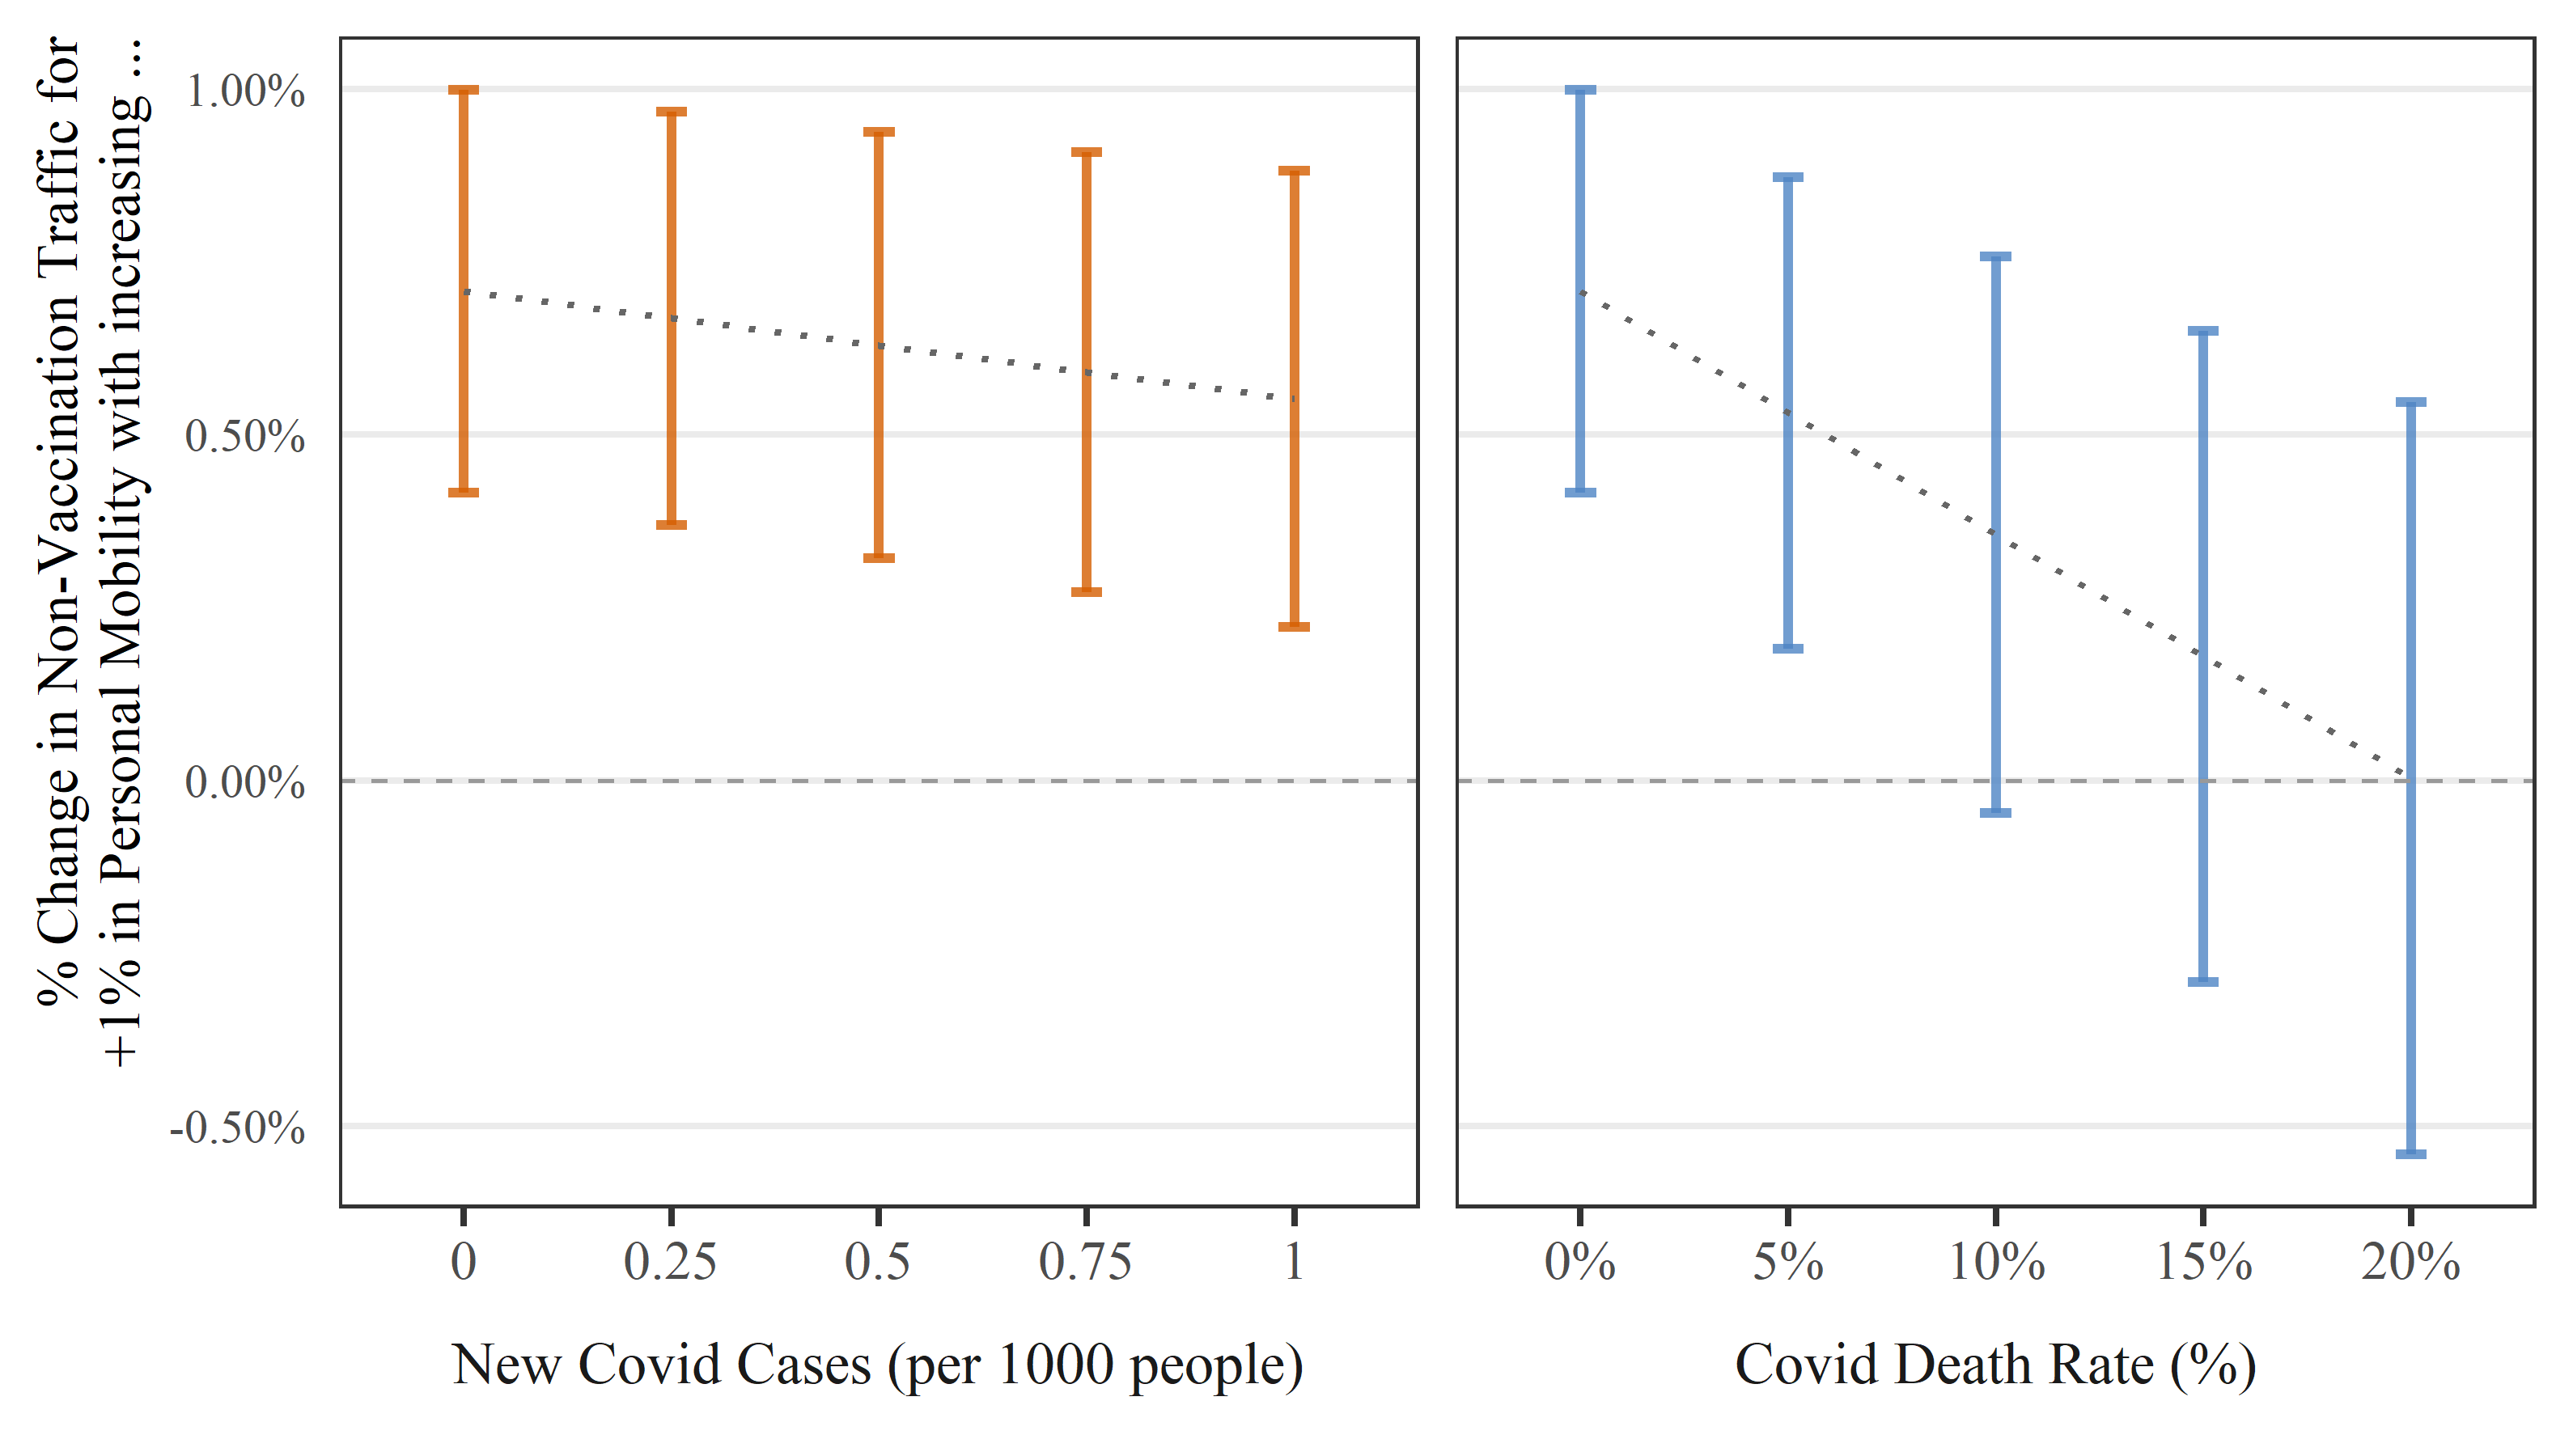
\includegraphics[scale=1]{Figures/VC2/Traffic-Moderation.png}     
    \label{fig:tfk_mod}
    % \floatfoot{\textbf{Figure Note:} 95\% confidence intervals depicted.}
\end{figure} 

\section{Conclusion} \label{Conclusion_VC2}
 Though recent technological innovations may have altered healthcare visits for good \citep{WSJ_checkup}, many aspects of medicine cannot happen virtually. Understanding the drivers of clinic traffic remains paramount, especially since a record number of patients delayed some type of care during the Covid-19 pandemic \citep{Findling2020}, where serious consequences can follow delayed or omitted vaccinations \citep{Salmon2015}. On top of this, the underlying causes of such concerns show few signs of abating as the emergence of Covid-19 variants continues to inhibit recovery \citep{WSJ_delta}.
 
 Combining observations from multiple sources allows us to evaluate how visits to healthcare clinics change with individual willingness to travel and signals of the current environment. As depicted in Figure \ref{fig:coef_plot}, increases in willingness to travel consistently drive large returns to vaccination traffic and smaller returns to all other traffic. Though the decreases in general clinic traffic do present some concerns, vaccination traffic seems immune to factors which depress demand for other care, such as such as state-wide stay-at-home orders and signals which might indicate a hazardous environment (e.g., a high Covid death rate). 
 
 We note the following limitations of our study. First, since observations of clinic traffic come from a vaccine management company, we observe only labels for “vaccination" or “non-vaccination" traffic. That is, we cannot identify different types of non-vaccination visits, even though some visits likely yield more value. Second, our data does not specify whether a non-vaccination visit happened virtually or in-person. Even so, Figure \ref{fig:model_free_vc2} shows non-vaccination traffic (virtual or otherwise) still had not recovered by the end of our study period. Said differently: Even with the broader acceptance and greater availability of telemedicine during the pandemic, such visits still cannot compensate for the drops we see in non-vaccination traffic. Third, we cannot observe the origin of a patient trip, though we do not believe patients cross multiple county lines to seek out primary care during the pandemic. Finally, we do not observe changes to clinic capacity in the wake of the pandemic. But since vaccination traffic returned to pre-pandemic baselines, we do not believe capacity restrictions hinder the recovery of non-vaccination traffic.
 
 Our findings yield several \textbf{implications} for research and practice. First, since mobility preferences strongly predict clinic traffic, operations managers can anticipate changes in traffic with greater precision by including such preferences in traffic prediction algorithms. Per one VaxCare representative: “Forecasting demand for vaccinations has been really tough recently. It is unclear what variables, if any, might be surrogates [for demand] which would reliably strengthen our forecasts." Our results show that personal mobility could be one such predictor. 
 
 Second, clinicians can find solace knowing that even if mobility (and thus traffic) declines again, patient discretion can help weather steep drops. The public health community championed the benefits of vaccines for decades \citep{Brewer2017}, and the efforts paid off during the summer of 2020. To hedge future downturns, clinicians should continue broadcasting the value of important services.
 
 Third, policy makers should remember traffic flows from mobility. To restore patient traffic and minimize delayed care -- by all means, keep clinics open -- but also address the circumstances depressing mobility. Aside from critically important traffic, people will stay home until it feels safe. On the flip side: To discourage mobility and keep people at home, transmit at least some precise information. For example, if public health agencies had transmitted precise, severe signals (e.g., the Covid death rate) along with the stay-at-home orders, compliance with stay-at-home orders might have been less of an issue. 
 
 Finally, healthcare researchers must acknowledge the role patient discretion plays in affecting operational outcomes. During the pandemic, clinics remained open while patients exercised discretion in ways many feared \citep{WSJ_famVacc}. But instead of the forecasted apocalypse, we find patients prioritized important services and shouldered some of the burden in maintaining their own wellness. Going forward, researchers should suggest ways firms can leverage the patient in the co-production of health.
 
 Covid-19 threatened the lives of many patients; weakened traffic threatened the jobs of many clinicians. But in healthcare, both pursue a joint goal. We show that by working together, even in the midst of a pandemic, patients and clinics can achieve such a goal: A healthy patient living in a healthy environment.

 \begin{figure}
    \centering
    \caption{An increase in personal mobility consistently corresponds to a much stronger return to vaccination traffic than to non-vaccination traffic.} %\medskip
    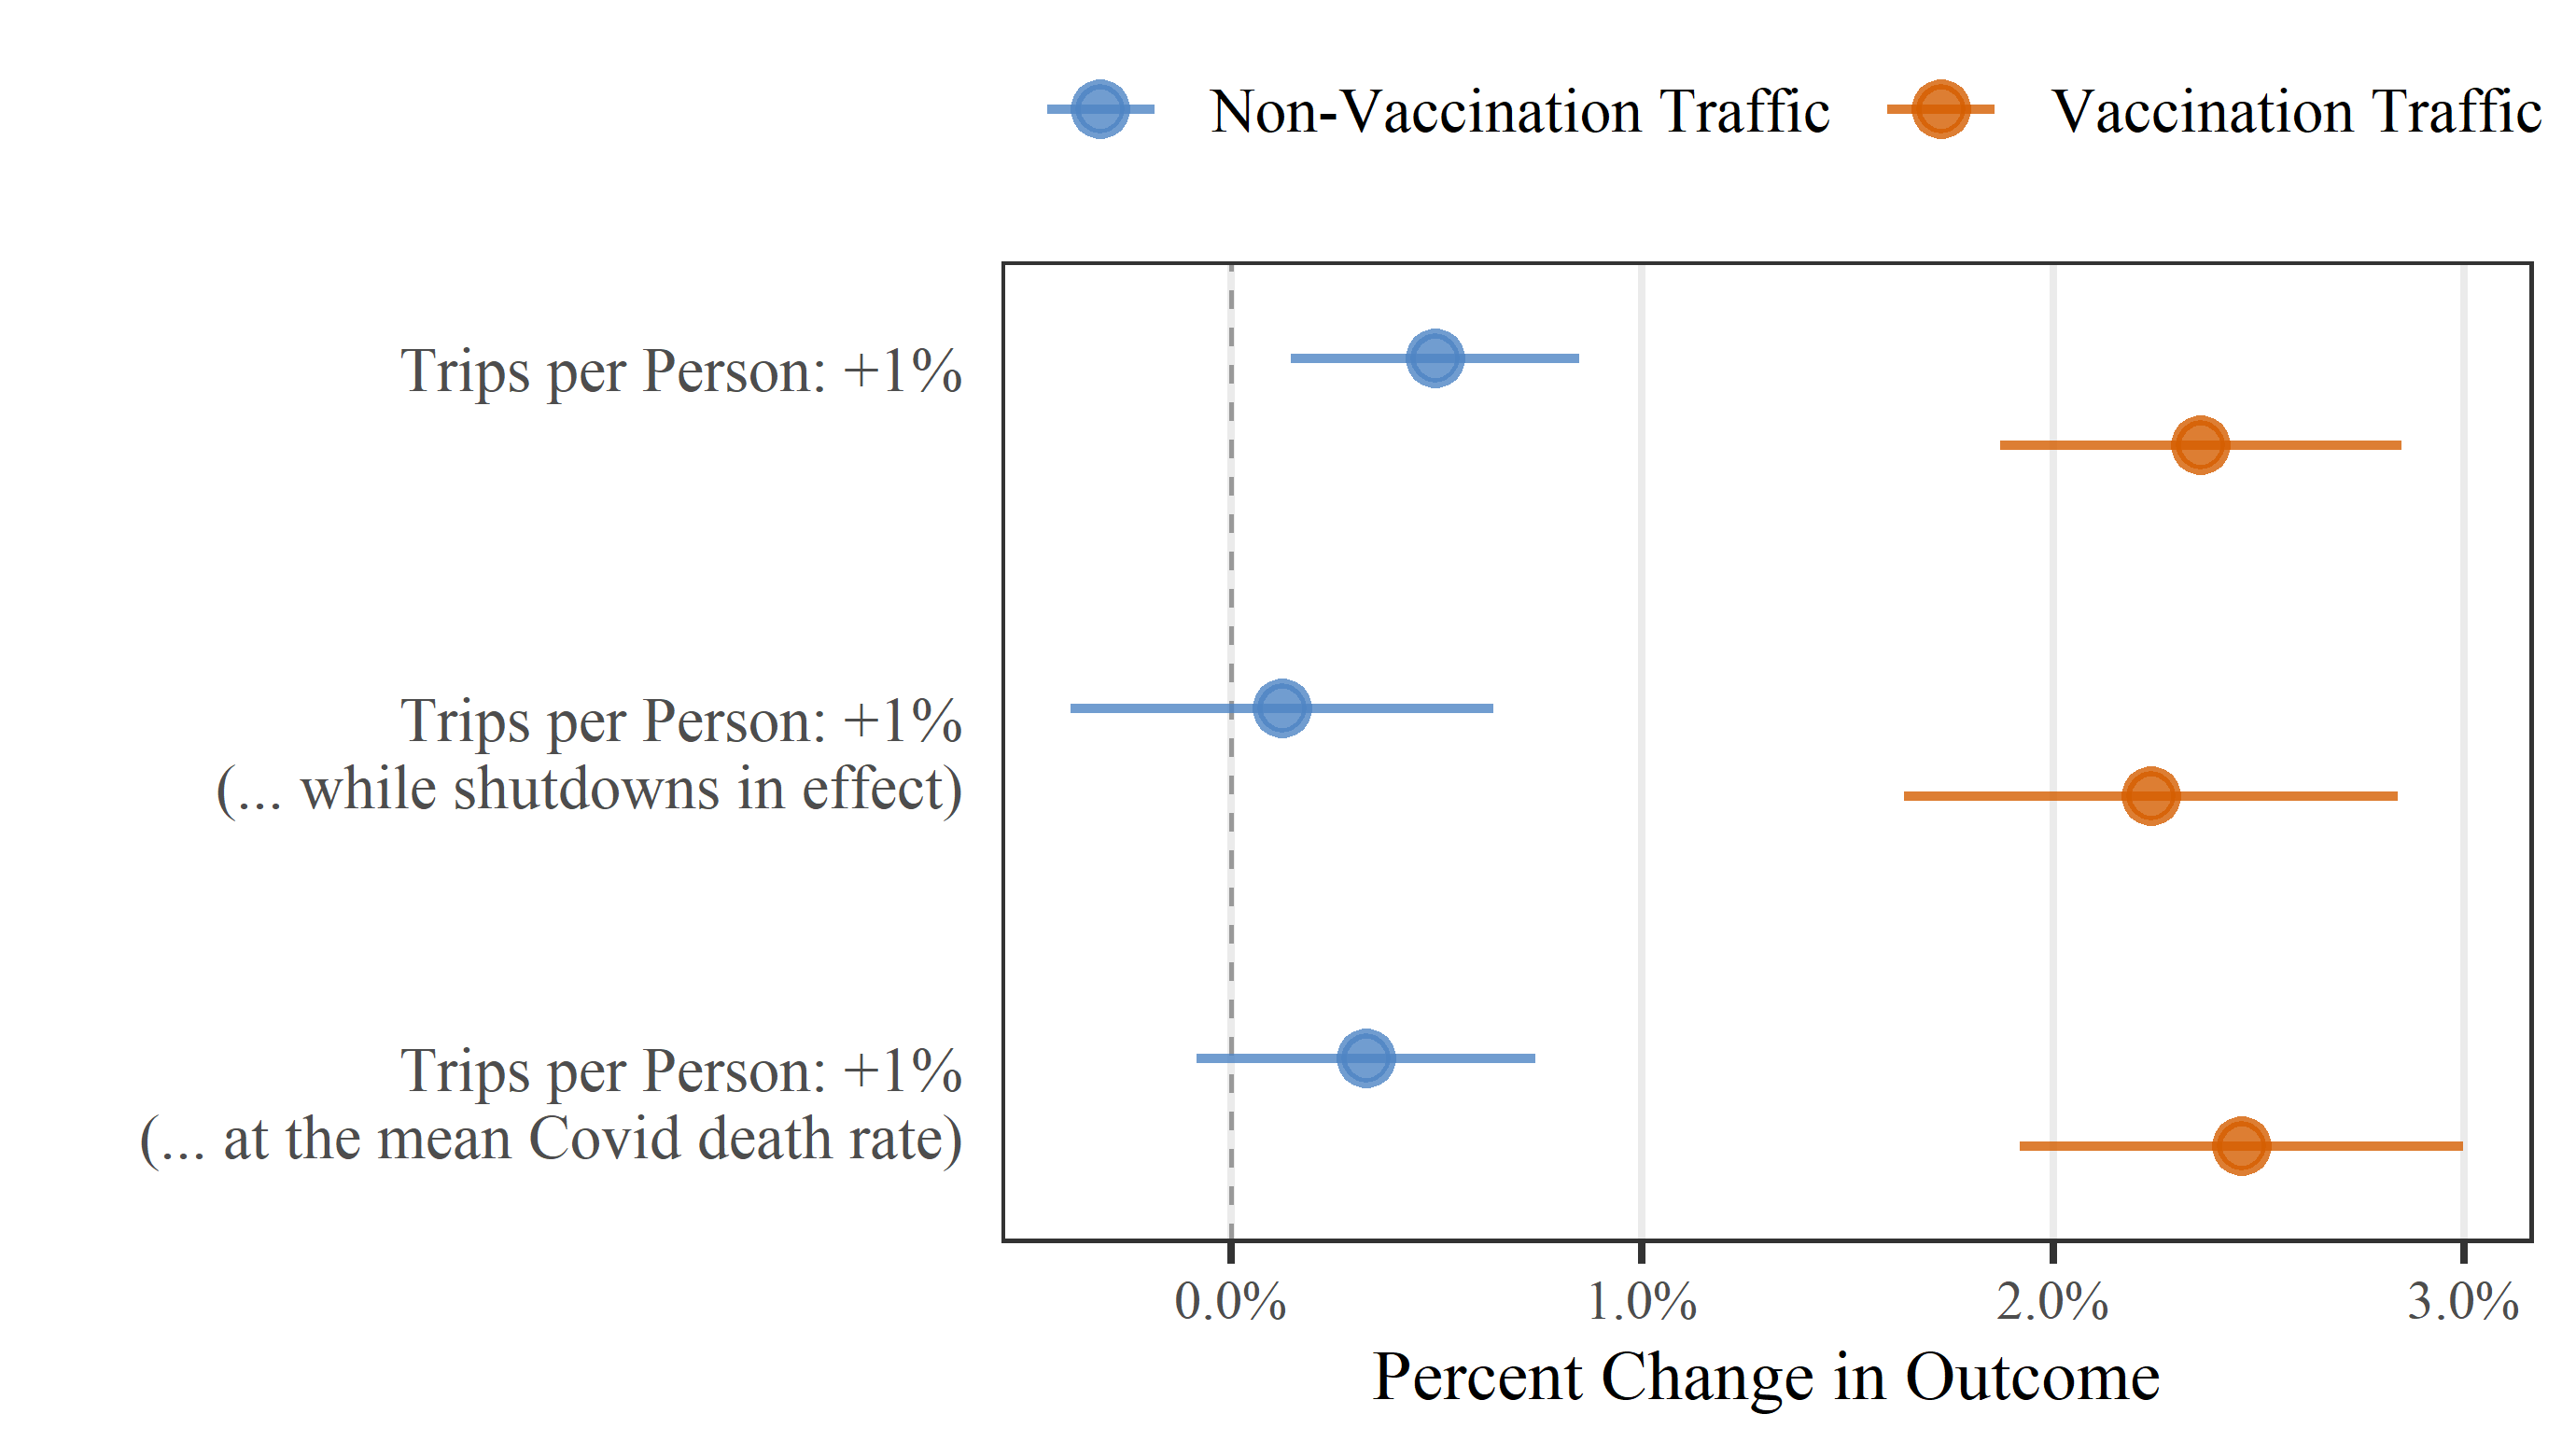
\includegraphics[scale=1]{Figures/VC2/Coef-Plot.png}     
    \label{fig:coef_plot}
    \floatfoot{\textbf{Figure Note:} The coefficient plot illustrates the marginal effect, or elasticity (and 95\% confidence intervals), of a change in personal mobility (i.e., Trips per Person) on clinic non-vaccination clinic traffic and vaccination traffic, as reported by the coefficients of Tables \ref{tab:H1H2} and \ref{tab:phoc}. The \nth{1} row illustrates a 1\% increase in personal mobility yields a more than 2\% increase in vaccination traffic versus a 0.5\% increase in non-vaccination traffic. The \nth{2} row depicts a significant drop in the effect of mobility on non-vaccination traffic while the state-wide stay-at-home orders are in effect, without a corresponding drop for vaccination traffic (Table \ref{tab:H1H2}, Columns 4 and 5). And the \nth{3} row illustrates that while the Covid death rate attenuates the effect of mobility on non-vaccination traffic, the effect of mobility on vaccination traffic seems immune to a such an effect (Table \ref{tab:phoc}).}
\end{figure}


\newpage
\bibliography{Bibliography/vc2_3feb22}

% Appendices
\appendix

% Switch to 1" title margins for appendices
\titlespacing{\chapter}{0in}{-.38in}{11pt}

% Appendix 1
\chapter{Chapter 1 Appendix -- Focusing Provider Attention} \label{app_cc}

\section{Pilot Study (2017)} \label{app_cc_pilot}
\subsection{Pilot Study Description}
In August 2017, VaxCare piloted a program aimed at increasing influenza vaccination in their clinic partners. This pilot program launched in the state of Florida and 101 clinics were recruited to participate for the 2017 flu vaccination season. The VaxCare program direction selected the treated clinics based on clinic history. Outside of the program, 68 other Florida clinics served as a control group. 

Two elements comprised the pilot program: Financial rebates (or incentives) and performance rankings. For the rebate component, VaxCare paid a rebate of \$1, \$2, or \$3 per shot for achieving various targets of flu shot growth. VaxCare set the three rebates to correspond to three tiers of Year-over-Year flu shot growth percentages. The second-tier threshold was typically 30\% Year-over-Year growth. Earned bonuses paid out at the end of the season. This incentive structure is similar to the Medicare penalties for poor performing clinics that accompanied the Affordable Care Act \citep[see][for discussion]{Zhang2016}. For the ranking component, VaxCare ranked the participating clinics based on their flu shot growth percentage and provided these as anonymous rankings to the clinics. Clinics could access both their progress to each incentive tier and their ranking information via a web portal.

Though extensive in its setup, the pilot study still suffered from potential selection bias: Clinics who agreed to participate likely had the most to gain from participating. Despite this limitation, our analysis of the pilot study directly informed the design of the field experiment in 2018, particularly the clinic consideration criteria. 

\subsection{Results: Percent Growth and Cumulative Shots}
By the end of the study, approximately a third of the 101 treated clinics reached some level of the incentive threshold: 63 clinics did not achieve any Tier; 3 clinics achieved Tier 1 (\$1 rebate per shot); 3 clinics achieved Tier 2 (\$2 rebate per shot); and 32 achieved Tier 3 (\$3 rebate per shot). Table \ref{tab:avg_diff} details the change in flu shots for clinics in the pilot study (“treated” clinics) versus the other clinics in Florida. The net effect of the study was a 33.54\% difference in flu shots between treatment and control. 

To test the statistical significance of this result, we ran a pooled Ordinary Least Squares model on clinic cumulative flu shots (\textit{CumShots}, specification below). The Treated indicator is set to 1 for the pilot study clinics and a 0 otherwise. The coefficient $\alpha_1$ captures the treatment effect and idiosyncratic shocks are captured in $\epsilon$. From Table \ref{tab:avg_diff}, we see that the clinics in the pilot study cumulatively administered 61.8 more shots than other Florida clinics outside the study ($p < 0.01$). Altogether, we find a positive outcome: Clinics in the pilot study increased their flu shots given between 2016 and 2017.

 \begin{table}
  \resizebox{.8\textwidth}{!}{ 
  \begin{threeparttable}[t]
   \centering
   \caption{Clinic Response to “Artificial” Ranks for Rebate and Control Groups}
    \begin{tabular}{lccccc}
          & \textbf{No. Clinics} & \multicolumn{2}{c}{\textbf{No. Flu Shots}} & \textbf{Pct. Growth} & \textbf{Net Effect} \\
          &       & \textbf{2016} & \textbf{2017} &       &  \\
    Control Clinics & 68    & 10,947 & 9,933 & -9.26\% &  \\
    Treated Clinics & 101   & 22,295 & 27,707 & 24.27\% & 33.54\% \\
    \end{tabular}%
    \medskip
    % \begin{tablenotes}
    %   \footnotesize
    %   \item \textbf{Table Note:} Clinic-robust standard errors in parentheses. All models include week fixed effects. 
    %   \item (*** $p < 0.01$, ** $p < 0.05$, + $p < 0.1$)
    % \end{tablenotes}
  \label{tab:net_effect}
  \end{threeparttable} }
 \end{table}

 \begin{equation} %\begin{split} %\end{split} 
       CumShots_{it} = \alpha_0 + \alpha_1 \mathbbm{1}\{TreatedClinic\}_{i} + \epsilon_{it}
 \end{equation} 

 \begin{table}
  \resizebox{.3\textwidth}{!}{ 
  \begin{threeparttable}[t]
   \centering
   \caption{Average Difference in Cumulative Shots for Treated Pilot Study Clinics}
    \begin{tabular}{lc}
          & (1) \\
          & \textbf{CumSPP} \\
          &  \\
    Treatment Effect ($\alpha_1$) & 61.8*** \\
          & (20.23) \\
          & [0.003] \\
          &  \\
    Observations & 3718 \\
    \# clinics & 169 \\
    \end{tabular}%
    \medskip
    \begin{tablenotes}
      \footnotesize
      \item \textbf{Table Note:} Table reports standard errors clustered by clinic (surrounded by parentheses) and two-sided p values [surrounded by brackets]. 
      \item (*** $p < 0.01$, ** $p < 0.05$, + $p < 0.1$)
    \end{tablenotes}
  \label{tab:avg_diff}
  \end{threeparttable} }
 \end{table}

\subsection{Pilot Study: Limitations}
The lack of random assignment represents the primary limitation of the pilot study. VaxCare’s goal for the pilot was to find clinics that would be willing to participate As such, growing clinics might have been more willing to participate and the clinics left out of the program might not serve as a valid control group. Separately, the design of the study highlights other limitations. For example, VaxCare added several of these treated clinics as partners late in the 2016 vaccination season. Establishing a baseline for these clinics meant estimating their vaccination history. Because of the subjective nature of this estimation, the Year-over-Year percent growth goals were not uniform across all the pilot study clinics. Finally, the treated clinics simultaneously received both the financial incentives and performance feedback. We do not know which treatment ultimately led to vaccination improvement – we only know that something did. Despite these limitations, the pilot study provided an initial exploration of the impact of financial incentives and rankings on vaccinations. The study also provided important inputs for the field experiment, including randomization. The following Appendix (Section \ref{app_exp_design}) discusses these inputs and how each informed our experimental design. 


\section{Field Experiment Design (2018)} \label{app_exp_design}
\subsection{Field Experiment: Design Considerations}
Informed by these outcomes from the pilot study, we worked with VaxCare to design and launch Compliance Care in 2018. This study included 145 clinics in 9 different states. Within each state, participant clinics were identified and then randomly assigned into three treatment arms: Rebate (49 clinics), Ranking (47 clinics), and Control (49 clinics). To accomplish this, we took the following steps. 

First, to determine the necessary sample size for our experiment, we performed a power analysis using the pilot study outcomes [$(\alpha,\beta)$ set at (0.05, 0.2)]. We calculated this value assuming a case where the control clinics exceed the performance of the treated clinics to be equivalent to “no effect of the treatment” using a one-tailed t-test. Our power analysis generated a required sample size of at least 42 control clinics and 44 clinics in each treatment arm. To ensure sufficient power to detect an effect, we rounded these counts up to 50 clinics in each group (150 clinics total).

Second, we worked closely with VaxCare to implement the clinic selection and randomization process. The baseline consideration criteria were the following: We only considered Family Practice or Internal Medicine clinics; to prevent spillover, the clinics could not have participated in the pilot study; to ensure an accurate baseline for performance, the clinic was required to be a VaxCare partner for the full 2017 flu vaccine season; and finally, to verify clinic ability and commitment to administering flu shots, the clinic had to have administered at least 150 flu shots during the 2017 flu shot season. 

Third, given these consideration criteria, VaxCare selected 9 states to serve as strata; within each state, VaxCare could then randomly assigned clinics to groups. Based on each state’s overall size, VaxCare set a target number of clinics for each state. The Compliance Care leadership team then solicited the state-level salesforce for recommendations on which clinics would be representative participants while still meeting the consideration criteria; this filtered out unresponsive or uncooperative partners. This group of clinics was then randomly sorted into treatment and control groups at the state-level. Finally, given each clinic’s assigned arm, the state-level representatives solicited each clinic’s participation; though participation required no additional cost on the part of the clinic, VaxCare insisted on receiving clinic consent. With this agreement in hand, Compliance Care commenced in August 2018. Please see Figure \ref{fig:exp_timeline} for the timing of these steps and the flu shot patterns for each group during the 2018 flu vaccine season. 

Given this approach, the field experiment addresses all the concerns of the pilot study. First, we applied strict selection criteria to establish a uniform assortment of clinics. This eliminated the requirement to estimate vaccination history and enabled robust measures of clinic performance. Second, the random assignment of geographically dispersed clinics mitigates the concern of selection bias due to either performance history or location. Third, our setup included the creation of a distinct, comparable control group, instead of using screened-out clinics as a proxy for a control. Fourth, separating the treatments (financial incentives and performance feedback) for each treatment group enables independent comparison between treatment and control and between treatments. Fifth, in the Rebate group, all clinics received identical incentive thresholds (10\%/15\%/20\% Year-over-Year growth). Finally, email notifications reduced the clinical burden to checking vaccination. In summary, the field experiment permits a robust evaluation of a flu shot intervention and builds on the initial findings of the pilot study. 

 \begin{figure}[htbp]
     \centering
     \caption{Experiment Timeline \& Weekly Flu Shots by Group} %\medskip
     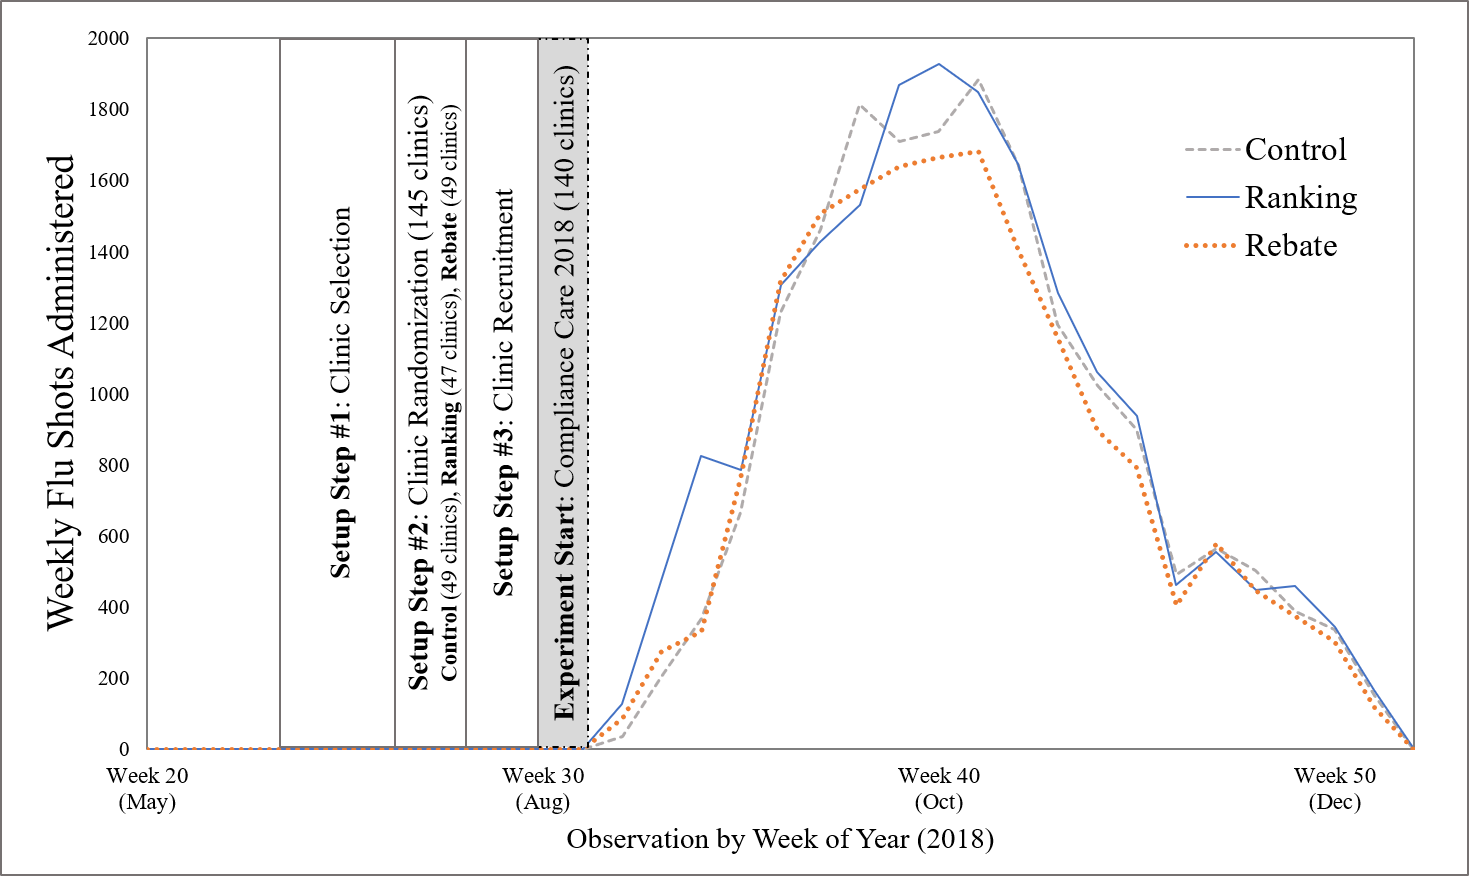
\includegraphics[scale=0.6]{Figures/CC/Figure B.1 - Experiment Timeline and Weekly Flu Shots by Group.png}     
     \label{fig:exp_timeline}
    %  \floatfoot{\textbf{Figure Note:}}
 \end{figure} 

\subsection{Field Experiment: Treatment Specifics}
As mentioned in Section \ref{cc_setup}, the treated clinics received an automated email each week from VaxCare. During the clinic recruitment phase, each clinic identified a staff member to VaxCare to serve as the point person for the program. In some cases, clinics identified their office manager as the point person, while in other cases, clinics selected a senior medical assistant who oversaw the clinic vaccination process. In any case, this point person served as the primary correspondent during the experiment while the clinic’s physicians received a carbon-copy of these reports as well. During recruitment, VaxCare carefully explained the format of these weekly emails, and clinics were encouraged to contact VaxCare’s customer care team with any follow-on questions. Based on our survey of these clinics, we know the contents of this email were reviewed regularly and shared generally with the rest of the staff – for example, at a weekly staff meeting. 

These emails contained the following elements. At the very top, the emails prominently highlighted each clinics’ specific treatment information, either flu shot percent growth or clinic rank. Next, clinics in both treatments received a growth table which outlined how many clinics shots were given by month either in 2017 (prior to the intervention) or in 2018 (during the intervention). Finally, the emails to the Rebate clinics also contained each vaccination threshold which corresponded to each of the three incentive tiers. For example, a clinic that administered 360 shots by the end of 2017 (as displayed in the growth table) would receive a Tier 1 threshold set at 396 shots corresponding to 10\% growth. The Rebate clinics received tiered incentive thresholds with rebates of \$1, \$2, and \$3 per shot awarded for achieving the targets set at 10\%, 15\%, and 20\% Year-over-Year flu shot growth. Rebate clinics who surpassed the tiered thresholds received that tier’s rebates for all shots given, including shots given before surpassing the threshold.


\section{Sensitivity and Test of Randomization} \label{app_cc_sens}
“The most credible and influential research designs use random assignment” \citep[p. 11]{Angrist2009}. Though ubiquitous in medicine, the Randomized Controlled Trial (RCT) has become more common in many academic disciplines, including economics, social science, and operations. And yet, even the “gold standard” of causal inference is not without assumptions. The purpose of this Appendix is to acknowledge any limitations and provide evidence that the findings presented in the remainder of the paper can still be considered valid. We refer interested readers to an extensive discussion of the limits of RCTs presented in \cite{Deaton2018}. 

As detailed in \cite{Deaton2018}, in order to estimate an unbiased average treatment effect (ATE), the researcher must assume balance between treated and non-treated subjects (or clinics). Proper randomization provides this balance in expectation \citep[p. 4]{Deaton2018}, assuming an infinite sample and an infinite number of randomizations. Practically, it is impossible to perform an infinite number of randomizations among an infinite sample, and any actual RCT must accept this as a limitation – that the estimated ATE is only unbiased in expectation. Researchers can, however, test for balance among observable covariates. 

Unfortunately, finding balance in observed covariates does not guarantee overall balance; the nature of unobserved covariates is just that – they are unobserved, and if any of these features are unbalanced and correlate with the treatment then the estimate of the ATE will in fact be biased. Thus, the previous assumption evolves to the following: If we can demonstrate balance in the observed covariates, then we argue that the likelihood is high that we have also achieved balance in the unobserved covariates leading to an unbiased estimate. This is akin to an assumption of unconfoundedness in the treatment effects literature \citep[e.g.,][]{Rubin1990} or more generally as the \cite{Heckman1985} assumption of selection on observables. The remainder of this addendum evaluates the balance between the Control, Ranking, and Rebate groups. Our analyses in this appendix can be \textbf{summarized} as follows: \\
1.	We cannot reject individual balance between means of 21 covariates for all 3 clinic groupings. \\
2.	We cannot reject joint balance between means of 21 covariates for all 3 clinic groupings.\\
3.	Without any further action (i.e., before trimming), we demonstrate acceptable common support in clinic treatment propensity as determined by 8 covariates. Only 3 clinics exhibit propensities outside of this support.\\
4.	After trimming these 3 clinics, and one additional clinic which lacks a comparison in the same state, we demonstrate excellent common support in clinic treatment propensity as determined by the same 8 covariates. We proceed to use this smaller clinic subset for two further tests.\\
5.	\textbf{Test 1}: When matching treated (Ranking/Rebate) to control clinics using the same 8 covariates, we see results in-line with our previous analyses: The Ranking clinics increase their flu shots by 15.8\% more than their matched Control clinics, and the result is statistically significant ($p < 0.05$). We also find no statistically significant effect between the Rebate clinics and their matched Control clinics.\\
6.	\textbf{Test 2}: After evaluating our panel regression models for clinic Percent Growth in flu shots (Specification 1) and clinic Shots per Patient-Population (Specification 4), our results are nearly identical to our findings before trimming: We find a statistically significant ($p < 0.05$) and similarly sized treatment effect for both outcome variables.\\

As a result, given that: (1) we cannot reject balance among our observable clinic measures; (2) we demonstrate that our clinics have common support; (3) we highlight the performance gap between Ranking and matched Control clinics which is consistent with our initial findings; and (4) our primary regression models are not sensitive to the inclusion or removal of clinics who lack common support; we conclude that we have demonstrated balance among our clinic groups and our treatment effect is unlikely to be biased. Nevertheless, we conservatively exclude these 4 clinics from our results which compare clinics between different groups.

\subsection{Test of Clinic Profiles: t-Test of clinic means}
As a first step, we want to rule out the possibility of differences in clinic profiles driving our results. To test these clinic profiles, we performed ‘t-Tests’ on the equality of the following variables between groups (Control versus Ranking, Ranking versus Rebate, and Control versus Rebate). The result of this operation is 63 total t-Tests (21 variables tested for 3 group comparisons). Here, we are testing the null hypothesis that these clinic profiles are the same in each of these categories. We restrict these comparisons to the clinics who completed the season as VaxCare partners. 

\begin{table}[htbp]
\resizebox{1\textwidth}{!}{ 
  \centering
  \caption{Variables Tested: t-Test, Hotelling’s T$^2$ Generalized Means Test}
    \begin{tabular}{ll}
    \textbf{2017 Variables} & \textbf{2018 Variables} \\
    Clinic: Percent Male Patients in 2017 & Clinic: Percent Male Patients in 2018 \\
    Clinic: Percent Patients over 65 in 2017 & Clinic: Percent Patients over 65 in 2018 \\
    Clinic: Average Patient Age in 2017 & Clinic: Average Patient Age in 2018 \\
    Clinic: Percent Medicare Patients in 2017 & Clinic: Percent Medicare Patients in 2018 \\
    Clinic: Percent Comm. Insurance Patients in 2017 & Clinic: Percent Comm. Insurance Patients in 2018 \\
    Clinic MD Count in 2017 & Clinic MD Count in 2018 \\
    Clinic Patient Count, Flu Shot Season 2017 & Clinic Patient Count, Flu Shot Season 2018 \\
          & Patient Count Difference, Flu Shot Season, 2017 to 2018 \\
    Clinic Patient Count, all of 2017 & Clinic Patient Count, all of 2018 \\
    Clinic: Flu Shot Total in 2017 & Clinic: Flu Shot Total in 2018 \\
    Clinic: Shots per Patient in 2017 & Clinic: Shots per Patient in 2018 \\
    \end{tabular}% 
  \label{tab:var_test} }
\end{table}%

The conclusion of these tests is that we cannot reject the null in 62 out of 63 tests ($p > 0.05$). The only test that rejects this null ($p < 0.05$) is the comparison for clinic percent of male patients between the Control and Rebate group in 2017. This rate is not greater than chance: With 63 tests we would expect a little over 3 of these tests to fail on average. As such, we claim balance on these observable covariates between all 3 groups.

\subsection{Test of Clinic Profiles: Hotelling’s T-squared generalized means test}
The previous test performs an individual test for each variable, but we can also test these equalities jointly. To do this, we performed “Hotelling’s T-squared generalized means test” to jointly compare the means of all above variables between the three groups \citep{Hotelling1931}. In this case, we cannot reject any of the null hypotheses that these groups are statistically equivalent ($p > 0.15$).

\subsection{Test of Clinic Profiles: Propensity to Treatment}
As a final test of the similarity of clinic profiles, we can calculate the propensity to being included as a treated clinic instead of a control clinic. We use this method to demonstrate that our treated (Ranking/Rebate) and control clinics share common support. The issue surrounding common support is discussed widely in the treatment effects literature; we refer readers to seminal papers in \cite{Caliendo2008} and \cite{Stuart2010}. 

Provided we can demonstrate we have common support between our treated and control clinics, our previous argument holds: Common support (or balance) in observed covariates increased the likelihood of common support in unobserved covariates, and we can compare groups to evaluate the effect of our treatment.

\subsection*{Evaluation of Common Support} 
In line with the treatment effects literature, we calculate each clinic’s propensity to be included as a treated clinic with a logistic regression model. The choice of included variables requires researcher discretion, but in line with \cite{Caliendo2008} and \cite{Angrist2009}, we choose variables that might simultaneously influence inclusion into the study and the treatment outcome. As such, we include the eight clinic-level variables listed in Table \ref{tab:var_input}. 

\begin{table}[htbp]
\resizebox{1\textwidth}{!}{ 
  \centering
  \caption{Variable Inputs: Evaluating Common Support \& Matching Outcomes}
    \begin{tabular}{lr}
    \textbf{2017 Variables} & \multicolumn{1}{l}{\textbf{2018 Variables}} \\
    Clinic MD Count in 2017 & \multicolumn{1}{l}{Clinic MD Count in 2018} \\
    Clinic Patient Count, Flu Shot Season 2017 & \multicolumn{1}{l}{Clinic Patient Count, Flu Shot Season 2018} \\
          & \multicolumn{1}{l}{Patient Count Difference, Flu Shot Season, 2017 to 2018} \\
    Clinic Patient Count, all of 2017 & \multicolumn{1}{l}{Clinic Patient Count, all of 2018} \\
    Clinic: Flu Shot Total in 2017 &  \\
    Clinic: Shots per Patient in 2017 &  \\
    \end{tabular}%
  \label{tab:var_input} } %
\end{table}%

We omit the demographic variables (e.g., percent male patients) as we do not have reason to believe these variables affected our outcome and they were not considered in our clinic consideration criteria. We do not include potential outcome measures (e.g., clinic shots per patient population in 2018), as the treated clinics had the opportunity to affect these outcomes. As in our main analysis, we restrict this analysis to clinics that started the vaccination season as VaxCare partners (N = 140). The following charts display the kernel density of the calculated propensities, both before and after trimming.

 \begin{figure}
     \centering
     \caption{Propensity to Treatment: Common Support Before Trimming} %\medskip
     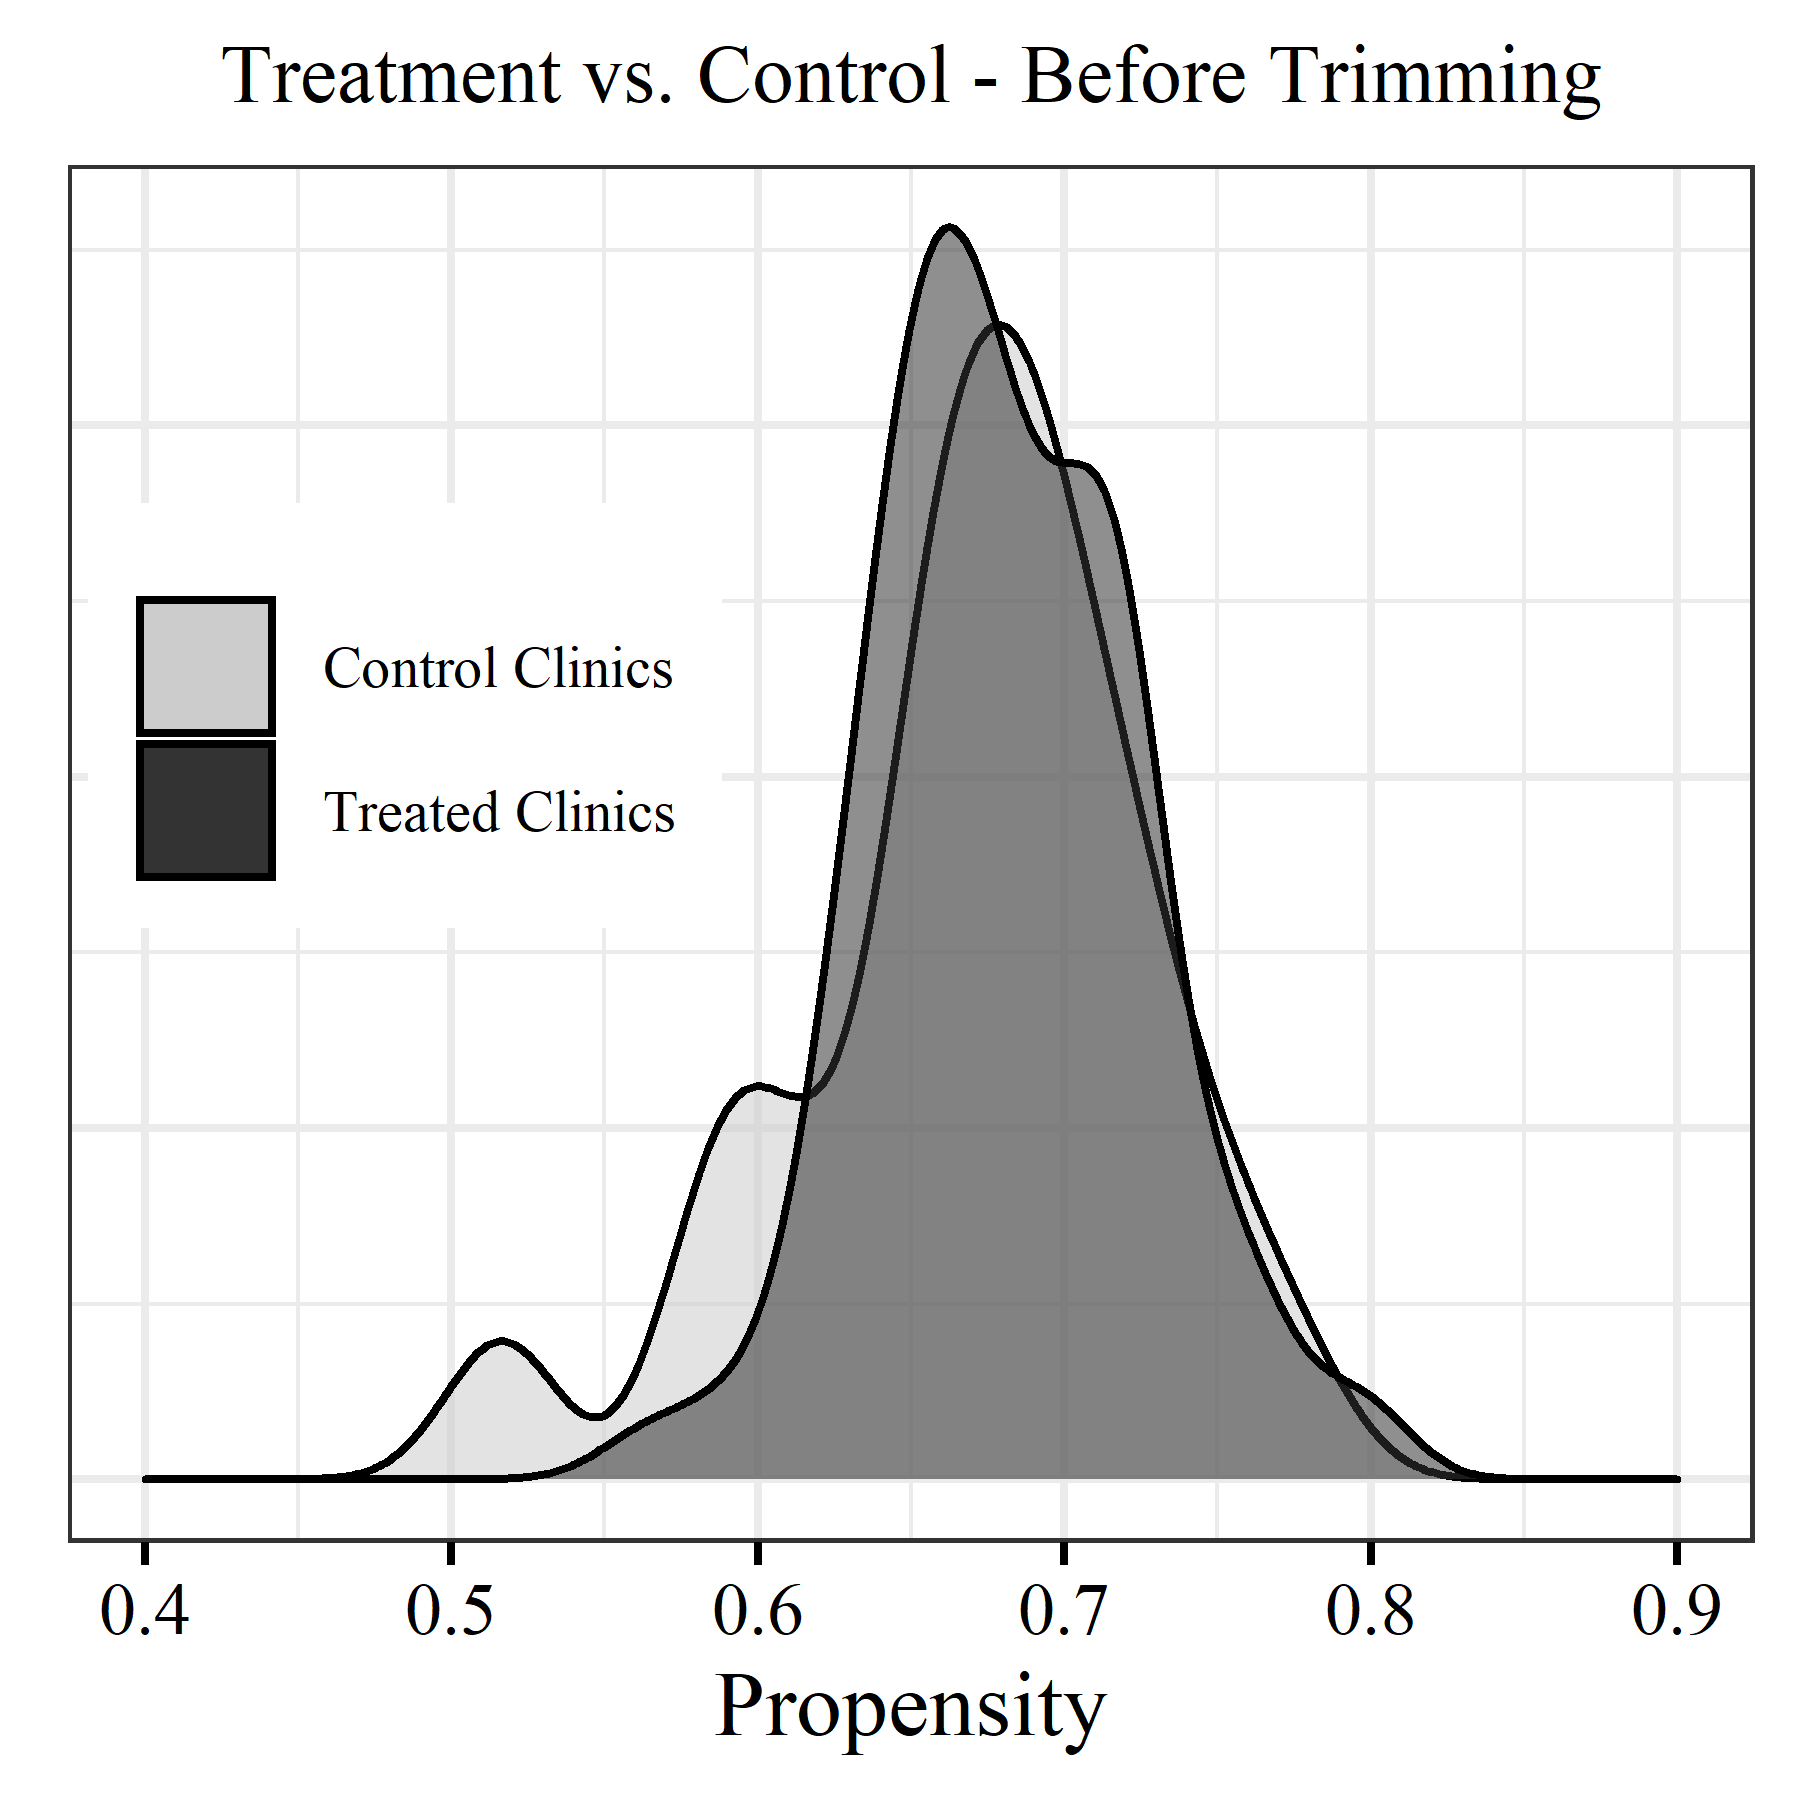
\includegraphics[scale=1]{Figures/CC/Figure C.1 (left).png}     
     \label{fig:pre_trim}
    %  \floatfoot{\textbf{Figure Note:}}
 \end{figure}  
 \begin{figure}
     \centering
     \caption{Propensity to Treatment: Common Support After Trimming} %\medskip
     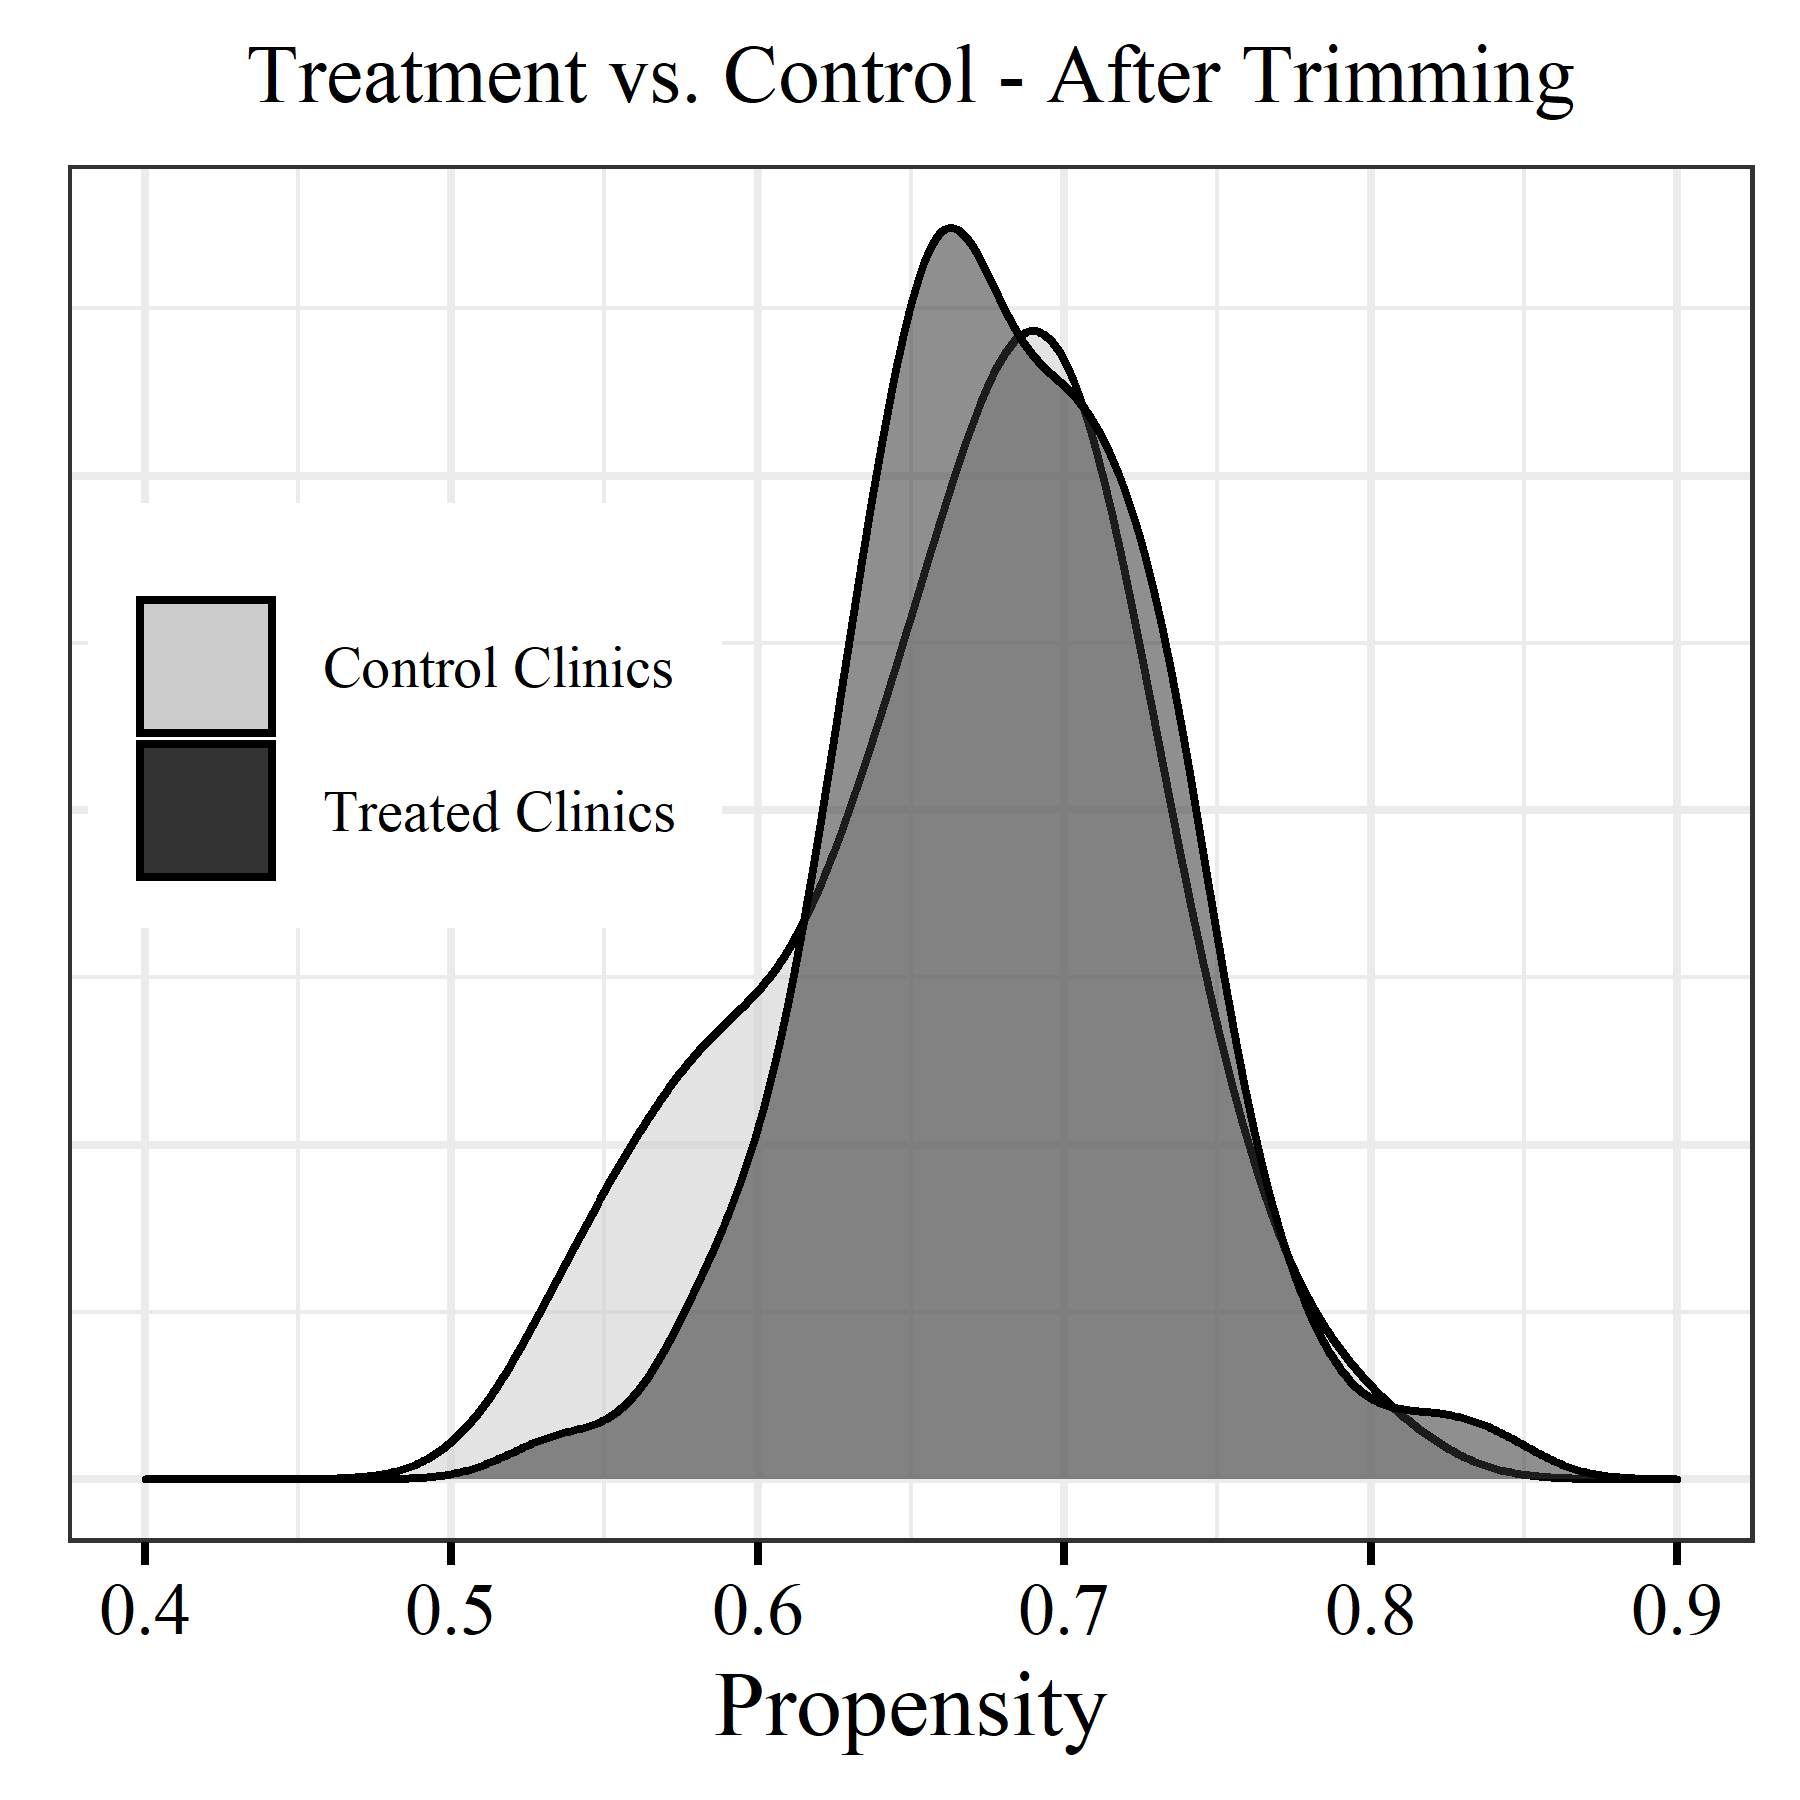
\includegraphics[scale=1]{Figures/CC/Figure C.1 (right).png}     
     \label{fig:post_trim}
    %  \floatfoot{\textbf{Figure Note:}}
 \end{figure} 

Figure \ref{fig:pre_trim} illustrates that there is common support for many of our clinics, even before trimming; there is significant overlap in the right-hand portion of the density graph. Nevertheless, there is one control clinic and two treated clinics with low propensity scores (less than 0.5) that have no comparable clinics. As these clinics do not possess comparable inputs, we should consider excluding them from our analysis. By dropping these clinics, we compromise our sample size but can more reasonably conclude that we are comparing similar clinics to one another. After dropping these three clinics, we are left with only one clinic in South Carolina. Our randomization was stratified by state, and as this clinic no longer has a comparable clinic in the state, the conservative approach is to also drop this clinic. 

After trimming these clinics, we recalculate our propensity to treatment, and this gives the density graph in Figure \ref{fig:post_trim}. As a result, we can reasonably conclude that we have common support for the above variables between our treated and our control clinics. Our final clinic distribution can be seen in Table \ref{tab:clinic_dist}. We proceed to evaluate the robustness of our outcomes to excluding these 4 clinics.

\begin{table}[htbp]
\resizebox{1\textwidth}{!}{ 
  \centering
  \caption{Average Treatment Effect for Matched Ranking and Rebate Clinics}
    \begin{tabular}{lcccc}
    \textbf{Treatment Group} & \textbf{Clinic Partners} & \textbf{Propensity Exclusion} & \textbf{State Exclusion} & \textbf{Final Clinic Count} \\
    Control & 46    & 1     & 1     & 44 \\
    Ranking & 46    & 2     & -     & 44 \\
    Rebate & 48    & -     & -     & 48 \\
    Clinic Total & 140   &       &       & 136 \\
    \end{tabular}%
  \label{tab:clinic_dist} } %
\end{table}%

\subsection*{Robustness Test 1: Matched Clinics} 
After excluding the four clinics above, we perform a test using a nearest neighbor matching method. This method is formally detailed in \cite{Abadie2006} with amplification in \cite{Abadie2011}. In short, nearest neighbor matching first determines the nearest neighbor using a weighted function of inputs. Once this neighbor is identified, the missing potential outcome is imputed by using the realized outcome of the nearest neighbor. The average treatment effect (ATE) is the average of the difference between realized and imputed outcomes for each clinic.

We match clinics and evaluate the outcome at the conclusion of our study. Starting with the Ranking clinics, we use the same eight variables listed in the previous table as inputs to match these clinics to the nearest, comparable Control clinics. We then do the same for the Rebate clinics. We also apply the bias adjustment for the continuous variables as discussed in \cite{Abadie2011}. Because patient counts, changes in patient count, and total doses serve to match these clinics, we test a separate, outcome independent of these factors: Year-over-Year percent growth in flu shots between 2017 and 2018. 

\begin{table}[htbp]
\resizebox{1\textwidth}{!}{ 
  \centering
  \caption{Average Treatment Effect for Matched Ranking and Rebate Clinics}
    \begin{tabular}{cccccc}
    \textbf{Treatment} & \textbf{Outcome} & \textbf{No. of observations} & \textbf{ATE} & \textbf{Standard error} & \textbf{Significance} \\
    Ranking & YoY Percent Growth & 44+44 = 88 & 0.158 & 0.0687 & $p < 0.05$ \\
    Rebate & YoY Percent Growth & 44+48 = 92 & 0.00152 & 0.0908 & $p > 0.10$ \\
    \end{tabular}%
  \label{tab:avg_te_2} } %
\end{table}%

After matching, the Rebate clinics show no statistically significant difference from their matched Control clinics, in line with our previous findings. For the Ranking clinics, however, we do see a statistically significant treatment effect: The Ranking clinics grew flu shots by 15.8\% more than their matched Control clinics. The magnitude of this effect is even more noteworthy, as only one comparison is made at the end of the year, whereas Specification 1 and Specification 4 evaluate the cumulative impact of the treatment over the entire season. We proceed to evaluate our regression models while only including the clinics with common support.

\subsection*{Robustness Test 2: Random Effects Regression Models} 
After excluding the clinics without common support, we are left with 136 clinics. We proceed to test the sensitivity of our findings to including or excluding the 4 clinics without common support. We tested our primary outcome measure (weekly percent growth of clinics over the 2018 vaccination season, or \textit{PercentGrowth} from Section \ref{emp_spec_pctGrowth}) and our alternate outcome measure (Cumulative Shots per Patient-Population, or \textit{CumSPP} from Section \ref{app_cc_alt_dv}). The econometric specifications follow the main text, and we continue to cluster the errors at the clinic level.
  \begin{equation} \tag{1} %\begin{split} %\end{split} 
      PercentGrowth_{it} = \beta_0 + \beta_1 TreatmentGroup_i + ClinicState_i + PatientCount_i + \epsilon_{it} 
  \end{equation}
  \begin{equation} \tag{4} \begin{split}
       CumSPP{it} = \beta_0 & + \beta_1 TreatmentGroup_i \times Year_t \\
       & + Year_t + TreatmentGroup_i \\ & + ClinicState_i + ClinicState_i \times Year_t + \epsilon_{it} 
  \end{split}  \end{equation}
  

Table \ref{tab:te_w_cs} presents the results of these regressions. Our results from Section \ref{cc_res_pctGrowth} (Specification 1) and Section \ref{app_cc_alt_dv} (Specification 4) are included in Columns 1 and 3 for comparison. The results from Column 2 show, on average, the Ranking clinics grew by approximately 7.9\% more than the Control clinics ($p < 0.05$) while the Rebate clinics show no meaningful difference in growth from the control. Furthermore, the results from Column 3 for Shots per Patient-Population show, on average, the Ranking clinics vaccinated 4.6\% more of their respective patient population than the Control clinics while the Rebate clinics show no meaningful difference. These results are nearly identical, though with slightly less precision in the smaller clinic sample. 

Given the results of both tests, along with our verification of common support, we conclude that we do have balance in our groups and our treatment effects are not sensitive to clinic profiles, affirming the validity and robustness of our randomization efforts. 

 \begin{table}
  \resizebox{1\textwidth}{!}{ 
  \begin{threeparttable}[t]
   \centering
   \caption{Treatment Effect of Compliance Care on Clinics with Common Support}
    \begin{tabular}{lcccc}
          & (1)   & (2)   & (3)   & (4) \\
          & \textbf{Percent Growth} & \textbf{Percent Growth} & \textbf{Shots per Patient Population } & \textbf{Shots per Patient Population } \\
    Econometric Model & Specification 1 & Specification 1 & Specification 4 & Specification 4 \\
          &       &       &       &  \\
    Ranking (Post-Treatment) & 0.0833** & 0.0793** & 0.0459** & 0.0460** \\
          & (0.0406) & (0.0395) & (0.0232) & (0.0224) \\
    Rebate (Post-Treatment) & 0.00219 & 0.00398 & 0.0125 & 0.0127 \\
          & (0.0399) & (0.0396) & (0.0235) & (0.0231) \\
          &       &       &       &  \\
    Observations & 2,720 & 2,800 & 5,712 & 5,880 \\
    \# clinics & 136   & 140   & 136   & 140 \\
    \end{tabular}%
    \medskip
    \begin{tablenotes}
      \footnotesize
      \item \textbf{Table Note:} Robust standard errors, clustered by clinic, in parentheses. Specification 1 includes clinic patient count and clinic state fixed effects. Specification 4 includes a year fixed effect, a state fixed effect, and an interaction between clinic state and year. 
      \item (*** $p < 0.01$, ** $p < 0.05$, + $p < 0.1$)
    \end{tablenotes}
  \label{tab:te_w_cs}
  \end{threeparttable} }
 \end{table}


\section{Alternate Dependent Variable} \label{app_cc_alt_dv}
When comparing clinic outcomes during Compliance Care, one must remember that clinics vary in size and capacity to deliver flu shots. Some clinics can administer 2,000 flu shots in a flu season, while others might only deliver 200 shots. Our primary dependent variable accounts for these factors by normalizing for Year-over-Year flu shot percent growth. As an alternate approach, we divide the cumulative number of weekly flu shots given by each clinics’ total patient population over the vaccination season (all patients who sought any clinic service) - Shots per Patient-Population. This metric addresses this consideration by normalizing by patient volume for large and small clinics. In line with a difference-in-differences approach, we interact a factor variable for treatment with an indicator variable for year. The resulting output measures the difference between the groups by year.  
  \begin{equation} \tag{4} \begin{split}
       CumSPP{it} = \beta_0 & + \beta_1 TreatmentGroup_i \times Year_t \\
       & + Year_t + TreatmentGroup_i \\ & + ClinicState_i + ClinicState_i \times Year_t + \epsilon_{it} 
  \end{split}  \end{equation}

We present the resulting Cumulative Shots per Patient-Population ($CumSPP$) for clinic $i$ in week $t$. The $TreatmentGroup$ variable is a factor variable with a level for each treatment (Control/Ranking/Rebate). The coefficient on the interaction variable specifies the performance difference between groups between 2017 and 2018. The $Year$ variable controls for the differing time trend between 2017 and 2018. We also include a state fixed effect and an interaction between Year and State to control for differing demand patterns in each geographic region each year. The idiosyncratic shocks which we have not controlled for are captured in $\epsilon$. 

As in Section \ref{cc_res_comp}, we conservatively focus on the clinics with common support (N = 136). The results of Table \ref{tab:te_alt_dv} show, on average, the Ranking clinics vaccinated approximately 5\% more of their respective patient population than the Control clinics while the Rebate clinics show no meaningful difference. As above, it appears the Ranking group outperformed the Control and the Rebate group. A Wald test confirms this by rejecting the null hypothesis that the Rebate clinics outperformed the Ranking clinics ($\beta_{1,rebate} >= \beta_{1,ranking}$; $p = 0.051$). Given this outcome and the outcome of Section \ref{cc_res_comp}, we confidently reject Hypothesis 1a and Hypothesis 2.

 \begin{table}
  \resizebox{0.5\textwidth}{!}{ 
  \begin{threeparttable}[t]
   \centering
   \caption{Treatment Effect of Compliance Care on Shots per Patient-Population (SPP)}
    \begin{tabular}{lc}
          & (1) \\
          & \textbf{Shots per Patient Population} \\
          &  \\
    Ranking (Post-Treatment) & 0.0459** \\
          & (0.0232) \\
    Rebate (Post-Treatment) & 0.0125 \\
          & (0.0235) \\
          &  \\
    Observations & 5,712 \\
    \# clinics & 136 \\
    \end{tabular}%
    \medskip
    \begin{tablenotes}
      \footnotesize
      \item \textbf{Table Note:} Robust standard errors, clustered by clinic, in parentheses. Model also includes a year fixed effect, a state fixed effect, and an interaction between clinic state and year fixed effect. 
      \item (*** $p < 0.01$, ** $p < 0.05$, + $p < 0.1$)
    \end{tablenotes}
  \label{tab:te_alt_dv}
  \end{threeparttable} }
 \end{table}

\section{Rank Response Sensitivity Analysis} \label{app_cc_rankResp_sens}
Given the results of Specification 3 in Section \ref{cc_res_rankResp}, we proceed to test the sensitivity of our conclusions for various definitions of first and last place. To evaluate our thresholds, we fix one parameter at the original definition and vary the other. For example, we reserve the high rank flag for clinics ranked in the top 5 but then relax and restrict the threshold for the bottom ranked clinics to test Last-Place Aversion. This test will also confirm or deny our lack of evidence for First-Place Loving behavior in the previous analysis (Section \ref{cc_res_rankResp}). We use the same outcome variable as defined in Section \ref{emp_spec_pctGrowth} (weekly shots per patient-population metric).

For various definitions of last place, please see Table \ref{tab:sensitivity_def_last}. We restrict our definition of last to only consider the lowest rank ($LowRank = 1$ if Rank $\in$ [46,46]) and relax our definition to consider clinics ranking in bottom 11 ranks ($LowRank = 1$ if Rank $\in$ [36,46]). We find statistically significant evidence for Last-Place Aversion even when relaxing the definition to consider clinics ranked in the bottom 10 ($p < 0.05$). Furthermore, evidence for Last-Place Aversion eventually vanishes. This is a welcome addition, as we would not expect Last-Place Aversion to exist for all definitions of last place. 

For various definitions of first place, please see Table \ref{tab:sensitivity_def_first}. We restrict our definition of first to only consider the top rank ($HighRank = 1$ if Rank $\in$ [1,1]) and relax our definition to consider the top 10 ranks ($HighRank = 1$ if Rank $\in$ [1,10]). The results are statistically significant when first place is defined as either of the top two ranks ($p < 0.01$ in Column 1 and $p < 0.10$ in Column 2); in all other definitions, the results are not statistically significant. Thus, if we restrict our definition of first place, we may have evidence of First-Place Loving behavior. However, in light of the robustness check in Section \ref{app_cc_grp_robust}, we cannot conclude this is not an artifact of some other unobservable behavior. Thus, we conclude that we do not have sufficient evidence to identify First-Place Loving behavior.

In summary, we find (1) our findings for First-Place Loving behavior are sensitive to our definition of “first” place and (2) our findings for Last-Place Aversion are not sensitive to our definition of “last place.” Thus, we find increasing evidence in support of Hypothesis 4. 

 \begin{table}
  \resizebox{1\textwidth}{!}{ 
  \begin{threeparttable}[t]
   \centering
   \caption{The Effect of Moving into a “Low” Rank on Weekly Shots per Patient-Population}
    \begin{tabular}{lcccccr}
          & (1)   & (2)   & (3)   & (4)   & (5)   & \multicolumn{1}{c}{(6)} \\
          & \textbf{WeekSPP} & \textbf{WeekSPP} & \textbf{WeekSPP} & \textbf{WeekSPP} & \textbf{WeekSPP} & \multicolumn{1}{c}{\textbf{WeekSPP}} \\
          &       &       &       &       &       &  \\
    Low Flag = 1 if Rank $\in$ & [36,46] & [37,46] & [38,46] & [39,46] & [40,46] & \multicolumn{1}{c}{[41,46]} \\
    Coeff.: Low Rank ($\pi_1$) & 0.00984 & 0.0136** & 0.0167*** & 0.0171*** & 0.0229*** & \multicolumn{1}{c}{0.0240***} \\
          & (0.00622) & (0.00606) & (0.00573) & (0.00596) & (0.00631) & \multicolumn{1}{c}{(0.00665)} \\
    High Flag = 1 if Rank $\in$ & [1,5] & [1,5] & [1,5] & [1,5] & [1,5] & \multicolumn{1}{c}{[1,5]} \\
    Coeff.: High Rank ($\pi_2$) & 0.00556 & 0.00557 & 0.00568 & 0.00551 & 0.00514 & \multicolumn{1}{c}{0.00517} \\
          & (0.00574) & (0.00571) & (0.00576) & (0.00579) & (0.00580) & \multicolumn{1}{c}{(0.00581)} \\
          &       &       &       &       &       &  \\
    Observations & 792   & 792   & 792   & 792   & 792   & \multicolumn{1}{c}{792} \\
    \# clinics & 46    & 46    & 46    & 46    & 46    & \multicolumn{1}{c}{46} \\
          &       &       &       &       &       &  \\
          & (7)   & (8)   & (9)   & (10)  & (11)  &  \\
          & \textbf{WeekSPP} & \textbf{WeekSPP} & \textbf{WeekSPP} & \textbf{WeekSPP} & \textbf{WeekSPP} &  \\
          &       &       &       &       &       &  \\
    Low Flag = 1 if Rank $\in$ & [42,46] & [43,46] & [44,46] & [45,46] & [46,46] &  \\
    Coeff.: Low Rank ($\pi_1$) & 0.0273*** & 0.0306*** & 0.0364*** & 0.0408*** & 0.0325*** &  \\
          & (0.00767) & (0.00936) & (0.00864) & (0.0116) & (0.00585) &  \\
    High Flag = 1 if Rank $\in$ & [1,5] & [1,5] & [1,5] & [1,5] & [1,5] &  \\
    Coeff.: High Rank ($\pi_2$) & 0.00461 & 0.00477 & 0.00480 & 0.00498 & 0.00492 &  \\
          & (0.00572) & (0.00568) & (0.00566) & (0.00562) & (0.00563) &  \\
          &       &       &       &       &       &  \\
    Observations & 792   & 792   & 792   & 792   & 792   &  \\
    \# clinics & 46    & 46    & 46    & 46    & 46    &  \\
    \end{tabular}%
    \medskip
    \begin{tablenotes}
      \footnotesize
      \item \textbf{Table Note:} This table details the specific effects of Ranking clinics moving into last place. All models include week fixed effects. Robust standard errors, clustered by clinic, in parentheses. The results from Table 2 (Column 2) have been duplicated in Column 7.
      \item (*** $p < 0.01$, ** $p < 0.05$, + $p < 0.1$)
    \end{tablenotes}
  \label{tab:sensitivity_def_last}
  \end{threeparttable} }
 \end{table}
 
  \begin{table}
  \resizebox{0.9\textwidth}{!}{ 
  \begin{threeparttable}[t]
   \centering
   \caption{The Effect of Moving into a “High” Rank on Weekly Shots per Patient-Population}
    \begin{tabular}{lccccc}
          & (1)   & (2)   & (3)   & (4)   & (5) \\
          & \textbf{WeekSPP} & \textbf{WeekSPP} & \textbf{WeekSPP} & \textbf{WeekSPP} & \textbf{WeekSPP} \\
          &       &       &       &       &  \\
    Low Flag = 1 if Rank $\in$ & [42,46] & [42,46] & [42,46] & [42,46] & [42,46] \\
    Coeff.: Low Rank ($\pi_1$) & 0.0273*** & 0.0273*** & 0.0273*** & 0.0273*** & 0.0273*** \\
          & (0.00765) & (0.00763) & (0.00767) & (0.00769) & (0.00767) \\
    High Flag = 1 if Rank $\in$ & [1,1] & [1,2] & [1,3] & [1,4] & [1,5] \\
    Coeff.: High Rank ($\pi_2$) & 0.0203*** & 0.0116+ & 0.00539 & 0.00768 & 0.00461 \\
          & (0.00687) & (0.00686) & (0.00590) & (0.00704) & (0.00572) \\
          &       &       &       &       &  \\
    Observations & 792   & 792   & 792   & 792   & 792 \\
    \# clinics & 46    & 46    & 46    & 46    & 46 \\
          &       &       &       &       &  \\
          & (6)   & (7)   & (8)   & (9)   & (10) \\
          & \textbf{WeekSPP} & \textbf{WeekSPP} & \textbf{WeekSPP} & \textbf{WeekSPP} & \textbf{WeekSPP} \\
          &       &       &       &       &  \\
    Low Flag = 1 if Rank $\in$ & [42,46] & [42,46] & [42,46] & [42,46] & [42,46] \\
    Coeff.: Low Rank ($\pi_1$) & 0.0273*** & 0.0275*** & 0.0277*** & 0.0276*** & 0.0275*** \\
          & (0.00764) & (0.00776) & (0.00780) & (0.00780) & (0.00773) \\
    High Flag = 1 if Rank $\in$ & [1,6] & [1,7] & [1,8] & [1,9] & [1,10] \\
    Coeff.: High Rank ($\pi_2$) & 0.00131 & 0.00557 & 0.00478 & 0.00480 & 0.00311 \\
          & (0.00482) & (0.00480) & (0.00449) & (0.00413) & (0.00437) \\
          &       &       &       &       &  \\
    Observations & 792   & 792   & 792   & 792   & 792 \\
    \# clinics & 46    & 46    & 46    & 46    & 46 \\
    \end{tabular}%

    \medskip
    \begin{tablenotes}
      \footnotesize
      \item \textbf{Table Note:} This table details the specific effects of Ranking clinics moving into first place. All models include week fixed effects. Robust standard errors, clustered by clinic, in parentheses.
      \item (*** $p < 0.01$, ** $p < 0.05$, + $p < 0.1$)
    \end{tablenotes}
  \label{tab:sensitivity_def_first}
  \end{threeparttable} }
 \end{table}

\newpage
\section{Rank Response – Robustness to Group Setting} \label{app_cc_grp_robust}
As discussed in Section \ref{rpf_robust}, we must consider mean reversion as an alternative mechanism for our findings. To test for this, we artificially ranked the clinics in the Control group (with respect to each other) and the clinics in the Rebate group (with respect to each other). We then applied our weekly shots per patient-population metric (defined in Section \ref{emp_spec_pctGrowth}) to the Control and Rebate clinics via Specification 2 and Specification 3, similar to a placebo test. 
\subsection{Specification 2: Results for Control and Rebate Clinics}
Table \ref{tab:art_ranks_reb_ctrl} contains the results of applying Specification 2 to the Rebate and Control groups. For the Rebate and Control group, not only are the coefficient magnitudes insignificant, but the coefficient signs are also different from the Ranking group, indicating a completely different function (i.e., not a U-shaped First-Place Loving/Last-Place Aversion curve) is (poorly) fitted to these two groups.

\begin{table}[!b]
  \resizebox{0.7\textwidth}{!}{ 
  \begin{threeparttable}[t]
   \centering
   \caption{Response to “Artificial” Ranks for Rebate and Control Groups}
    \begin{tabular}{lccc}
          & (1)   & (2)   & (3) \\
          & \textbf{WeekSPP} & \textbf{WeekSPP} & \textbf{WeekSPP} \\
          &       &       &  \\
    Clinic Group & Ranking & Rebate & Control \\
    Rank, previous week ($\lambda_1$) & -0.00209*** & 0.000867 & -0.000163 \\
          & (0.000648) & (0.000782) & (0.000940) \\
    Rank$^2$, previous week ($\lambda_2$) & 5.34e-05*** & -1.83e-05 & -4.98e-06 \\
          & (1.36e-05) & (2.10e-05) & (2.66e-05) \\
          &       &       &  \\
    Observations & 792   & 823   & 742 \\
    \# clinics & 46    & 48    & 44 \\
    \end{tabular}%
    \medskip
    \begin{tablenotes}
      \footnotesize
      \item \textbf{Table Note:} This table the parameter estimates from Model 2 for all clinic groups: Ranking, Rebate, and Control. Robust standard errors, clustered by clinic, in parentheses. All models include week fixed effects. 
      \item (*** $p < 0.01$, ** $p < 0.05$, + $p < 0.1$)
    \end{tablenotes}
  \label{tab:art_ranks_reb_ctrl}
  \end{threeparttable} }
 \end{table}

\subsection{Specification 3: Results for Control Clinics}
When testing for Last-Place Aversion, we test any definition of last place down to clinics that were ranked in the bottom half (ranks greater than or equal to 23 out of 46 Control clinics). In this case, we do not see any statistically significant results among the Control clinics for any of these definitions for Model 3. When testing for First-Place Loving behavior, we test for all definitions of first place to clinics ranked in the top 10; we do see instances of statistically significant results in the top ranks (Columns 1, 2 and 3 under Table \ref{tab:move_high_rank}). For example, when defining “first” as the top rank only, the control clinics respond to non-existent ranks with a +1.21\% change in shots per patient-population ($p < 0.05$). 

\begin{table} %[!b]
  \resizebox{0.9\textwidth}{!}{ 
  \begin{threeparttable}[t]
   \centering
   \caption{The Effect of Moving into a “High” Rank on Weekly Shots per Patient-Population}
    \begin{tabular}{lccccc}
          & (1)   & (2)   & (3)   & (4)   & (5) \\
          & \textbf{WeekSPP} & \textbf{WeekSPP} & \textbf{WeekSPP} & \textbf{WeekSPP} & \textbf{WeekSPP} \\
    Clinic Group & Control & Control & Control & Control & Control \\
    Econometric Model & Specification 3 & Specification 3 & Specification 3 & Specification 3 & Specification 3 \\
          &       &       &       &       &  \\
    High Flag = 1 if Rank $\in$ & [1,1] & [1,2] & [1,3] & [1,4] & [1,5] \\
    Coeff.: High Rank ($\pi_2$) & 0.0121** & 0.0105*** & 0.00901** & 0.00397 & 0.00140 \\
          & (0.00560) & (0.00311) & (0.00384) & (0.00458) & (0.00505) \\
          &       &       &       &       &  \\
    Observations & 742   & 742   & 742   & 742   & 742 \\
    \# clinics & 46    & 46    & 46    & 46    & 46 \\
    \end{tabular}%
    \medskip
    \begin{tablenotes}
      \footnotesize
      \item \textbf{Table Note:} This table details the parameter estimates from Model 3 for the Control group. Robust standard errors, clustered by clinic, in parentheses. All models include week fixed effects. 
      \item (*** $p < 0.01$, ** $p < 0.05$, + $p < 0.1$)
    \end{tablenotes}
  \label{tab:move_high_rank}
  \end{threeparttable} }
 \end{table}

\subsection{Specification 3: Results for Rebate Clinics}
When testing for LPA, we test any definition of last place down to clinics that were ranked in the bottom half (ranks greater than or equal to 24 out of 48 Rebate clinics). In this case, we do not see any statistically significant results among the Rebate clinics for any of these definitions. When testing for First-Place Loving behavior, we test for all definitions of first place to clinics ranked in the top 10. We do not see any statistically significant results among the Rebate clinics for any of these definitions.

\subsection{Overall Test Implications}
Given these results, we continue to find strong evidence for Last-Place Aversion: The behavior we measure among the Ranking clinics is unique to those clinics and does not manifest in either the Control or Rebate clinics, who received no rank information. However, these results do indicate that we are not explaining the performance of the clinics who achieve a high rank, as we observe similar behavior among Control clinics who received no rank information. Market saturation presents one possible reason for why we do not observe First-Place Loving behavior: Top ranked clinics may lack room to improve as they vaccinate their respective patient populations. 

Thus, in summary, we do not find enough to robustly claim evidence for Hypothesis 3 and First-Place Loving behavior, however, we do find strong evidence to support Hypothesis 4 and the presence of Last-Place Aversion. 


% Appendix 2
\chapter{Chapter 2 Appendix -- Task Selection and Patient ``Pick-up"}

% \newpage
\section{Data Trimming} \label{app_pu_Trim}
 Because we are interested in the impact of group familiarity, we first remove all observations where only one provider was observed during a given hour. Such observations are of a “group” of 1 with no possible familiarity. Second, to mitigate the presence of some outliers in the data which may follow data entry errors or miscoding, we trim the data to contain only up to the 97th percentile of patient length of stay (dropping 1,276 observations with visits longer than about 24 hours) and any observations which contain patient wait times greater than 400 minutes (approximately the 99th percentile, dropping 392 observations). Additionally, 72 observations do not include an indication of patient severity upon arrival to the ED. As such information is critical to a physician’s decision to pick-up a patient, we also drop such observations. Finally, we drop 6 observations which list the discharge time before the pick-up time and 208 observations where the pick-up is listed as the same the the arrival time, as duration analysis cannot be performed on observations with zero time-to-failure. After trimming, we are left with 40,617 observations. 
 

% \newpage
\section{Example Panels} \label{app_pu_examples}

\begin{table}[htbp]
  \resizebox{1\textwidth}{!}{ 
  \begin{threeparttable}[t]
   \centering
   \caption{Hypothetical ED Panel, Sorted by Patient Pick-up Time}
    \begin{tabular}{ccccccccccccc}
    \textbf{Pick-up} & \textbf{Pick-up} & \textbf{Pick-up} &       & \textbf{Group} & \textbf{Phys.} & \textbf{Pair-1} & \textbf{Pair-2} & \textbf{Pair-3} & \textbf{Fam:} & \textbf{Fam:} & \textbf{Fam:} & \textbf{Average} \\
    \textbf{Time} & \textbf{Hour} & \textbf{Phys. ID} & \textbf{Phys. Exp.} & \textbf{Size (hr)} & \textbf{Group (hr)} & \textbf{IDs} & \textbf{IDs} & \textbf{IDs} & \textbf{Pair1} & \textbf{Pair2} & \textbf{Pair3} & \textbf{Familiarity} \\
          &       &       &       &       &       &       &       &       &       &       &       &  \\
    9:23 AM & 9     & 57    & 1     & 2     & 57, 83 & (57, 83) &       &       & 1     &       &       & 1.00 \\
    9:42 AM & 9     & 83    & 4     & 2     & 57, 83 & (57, 83) &       &       & 2     &       &       & 2.00 \\
    9:44 AM & 9     & 83    & 5     & 2     & 57, 83 & (57, 83) &       &       & 3     &       &       & 3.00 \\
    9:55 AM & 9     & 57    & 2     & 2     & 57, 83 & (57, 83) &       &       & 4     &       &       & 4.00 \\
    9:56 AM & 9     & 57    & 3     & 2     & 57, 83 & (57, 83) &       &       & 5     &       &       & 5.00 \\
    10:06 AM & 10    & 83    & 6     & 3     & 57, 69, 83 & (57, 69) & (57, 83) & (69, 83) & 1     & 6     & 8     & 5.00 \\
    10:11 AM & 10    & 69    & 3     & 3     & 57, 69, 83 & (57, 69) & (57, 83) & (69, 83) & 2     & 7     & 9     & 6.00 \\
    10:30 AM & 10    & 57    & 4     & 3     & 57, 69, 83 & (57, 69) & (57, 83) & (69, 83) & 3     & 8     & 10    & 7.00 \\
    \end{tabular}%
    \medskip
    \begin{tablenotes}
      \footnotesize
      \item \textbf{Table Note:} The table represents a hypothetical snapshot of our data, sorted by patient pick-up time. \textbf{Pick-up: Phys. ID} is the identifier of the physician picking up the patient at the \textbf{Pick-up Time}. \textbf{Phys. Exp.} is a cumulative count of the number of patients picked up by the physician while working in a group. The physician group [Phys. Group (hr)] of size [\textbf{Group Size (hr)}] is defined for the \textbf{Pick-up Hour} as “any physician who picked up a patient that hour.” A physician group of size $N$ yields “$N$ choose 2” pairwise combinations (e.g., \textbf{Pair-1 IDs}). Each pair of physicians has a familiarity count (e.g., \textbf{Fam: Pair1}). Each group has a mean pairwise familiarity (Average Familiarity). In the example above, physician pair (57, 83) and pair (57, 69) had not worked together before, and so pairwise familiarity starts at zero. In contrast, Physicians 69 and 83 had worked together before the panel, and so they already possessed some level of familiarity.
    \end{tablenotes}
%   \label{tab:add_label}
  \end{threeparttable} }
 \end{table}

\begin{table}[htbp]
  \resizebox{1\textwidth}{!}{ 
  \begin{threeparttable}[t]
   \centering
   \caption{Hypothetical Physician Panel, Sorted by Patient Pick-up Time}
    \begin{tabular}{cccccccc}
    \textbf{Pick-up} & \textbf{Pick-up} & \textbf{Pick-up:} &       &       & \textbf{Pick up New Patient?} & \textbf{Group} & \textbf{Phys.} \\
    \textbf{Time} & \textbf{Hour} & \textbf{Phys. ID} & \textbf{Phys. Exp.} & \textbf{Shift ID} & \textbf{1 - “Yes"; 0 - “No" } & \textbf{Size (hr)} & \textbf{Group (hr)} \\
          &       &       &       &       &       &       &  \\
    3:45 PM & 15    & 4     & 1     & 1     & 1     & 3     & 4, 45, 76 \\
    3:46 PM & 15    & 4     & 2     & 1     & 1     & 3     & 4, 45, 76 \\
    3:47 PM & 15    & 4     & 3     & 1     & 1     & 3     & 4, 45, 76 \\
    3:54 PM & 15    & 4     & 4     & 1     & 1     & 3     & 4, 45, 76 \\
    5:04 PM & 17    & 4     & 5     & 1     & 1     & 4     & 4, 45, 68, 76 \\
    9:28 PM & 21    & 4     & 6     & 1     & 1     & 2     & 4, 68 \\
    10:31 PM & 22    & 4     & 7     & 1     & 1     & 3     & 4, 67, 68 \\
    10:32 PM & 22    & 4     & 8     & 1     & 0     & 3     & 4, 67, 68 \\
          &       &       &       &       &       &       &  \\
    4:59 PM & 16    & 4     & 9     & 2     & 1     & 3     & 4, 52, 69 \\
    5:03 PM & 17    & 4     & 10    & 2     & 1     & 2     & 4, 52 \\
    5:04 PM & 17    & 4     & 11    & 2     & 1     & 2     & 4, 52 \\
    6:13 PM & 18    & 4     & 12    & 2     & 1     & 3     & 4, 26, 52 \\
    6:46 PM & 18    & 4     & 13    & 2     & 1     & 3     & 4, 26, 52 \\
    6:47 PM & 18    & 4     & 14    & 2     & 1     & 3     & 4, 26, 52 \\
    10:00 PM & 22    & 4     & 15    & 2     & 1     & 3     & 4, 52, 64 \\
    10:27 PM & 22    & 4     & 16    & 2     & 0     & 3     & 4, 52, 64 \\
          &       &       &       &       &       &       &  \\
    8:09 AM & 8     & 4     & 17    & 3     & 1     & 2     & 4, 65 \\
    8:44 AM & 8     & 4     & 18    & 3     & 1     & 2     & 4, 65 \\
    10:16 AM & 10    & 4     & 19    & 3     & 1     & 3     & 4, 15, 65 \\
    1:02 PM & 13    & 4     & 20    & 3     & 1     & 3     & 4, 15, 65 \\
    2:38 PM & 14    & 4     & 21    & 3     & 0     & 4     & 4, 11, 15, 89 \\
    \end{tabular}%
    \medskip
    \begin{tablenotes}
      \footnotesize
      \item \textbf{Table Note:} The table represents a hypothetical snapshot of our data, focusing on one physician ID and sorted by patient pick-up time. \textbf{Phys. ID} is the identifier of the physician picking up the patient at the \textbf{Pick-up Time}. \textbf{Phys. Exp.} is a cumulative count of the number of patients picked up by the physician while working in a group. \textbf{Shift ID} identifies each unique shift. The physician group [\textbf{Phys. Group (hr)}] of size \textbf{Group Size (hr)} is defined for the \textbf{Pick-up Hour} as “any physician who picked up a patient that hour.” The \textbf{Pick up New Patient} column is an indicator variable which indicates whether the provider picked up another patient after the focal patient.
    \end{tablenotes}
%   \label{tab:add_label}
  \end{threeparttable} }
 \end{table}

% \newpage
\section{Full Regression Results} \label{pu_full_reg}

\begin{table}[htbp]
  \resizebox{1\textwidth}{!}{ 
  \begin{threeparttable}[t]
   \centering
   \caption{Full Regression Results for All Hypotheses}
    \begin{tabular}{lcccccc}
          & (1)   & (2)   & (3)   & (4)   & (5)   & (6) \\
    Output Variable & \textbf{Pick-up Rate} & \textbf{Pick-up Likelihood} & \textbf{Multitasking} & \textbf{Wait Time} & \textbf{Processing Time} & \textbf{Length of Stay} \\
    Model & Linear FE & Chamberlain RE Probit & Linear FE & AFT Duration & AFT Duration & AFT Duration \\
    Estimation Method & Coefficient/APE & Coefficient & Coefficient/APE & Coefficient & Coefficient & Coefficient \\
          &       &       &       &       &       &  \\
    \textit{Average Familiarity} & 0.0319*** & 0.0959*** & 0.141*** & -0.0155** & -0.0000725 & -0.00330 \\
          & (0.00796) & (0.0134) & (0.0168) & (0.00646) & (0.00392) & (0.00325) \\
          & [0.000128] & [0]   & [0]   &       &       &  \\
    \textit{Waiting Room Occupancy (lag)} & 0.0452*** & -0.0117*** & 0.000254 & 0.0931*** & -0.00577*** & 0.0237*** \\
          & (0.00302) & (0.00395) & (0.00435) & (0.00213) & (0.00105) & (0.000873) \\
          & [0]   & [0.00308] & [0.954] &       &       &  \\
    \textit{ED Seen Occupancy (lag)} & 0.0154*** & 0.0575*** & 0.145*** & 0.0129*** & 0.00567*** & 0.00705*** \\
          & (0.00183) & (0.00424) & (0.00507) & (0.00163) & (0.000875) & (0.000750) \\
          & [0]   & [0]   & [0]   &       &       &  \\
    \textit{Physician Hours into Shift} & -0.200*** & -0.619*** & 0.634*** & -0.00153 & -0.0225*** & -0.0146*** \\
          & (0.00607) & (0.0247) & (0.00991) & (0.00240) & (0.00170) & (0.00125) \\
          & [0]   & [0]   & [0]   &       &       &  \\
    \textit{Physician Experience (linear)} & 0.0382 & 0.130 & 0.380*** & 0.122*** & 0.0729*** & 0.0829*** \\
          & (0.0414) & (0.115) & (0.0755) & (0.0304) & (0.0186) & (0.0161) \\
          & [0.359] & [0.256] & [2.46e-06] &       &       &  \\
    \textit{Physician Experience (quadratic)} & 0.00364 & -0.0112 & -0.0468*** & -0.0142*** & -0.00744*** & -0.00871*** \\
          & (0.00589) & (0.0133) & (0.0121) & (0.00464) & (0.00283) & (0.00245) \\
          & [0.538] & [0.402] & [0.000214] &       &       &  \\
    \textit{Physician Multitasking (lag)} &       & 0.0313** &       &       &       &  \\
          &       & (0.0133) &       &       &       &  \\
          &       & [0.0185] &       &       &       &  \\
    \textit{Team Size: 2 physicians} & -0.216 & 0.723 & 1.188** & 0.237*** & 0.191** & 0.134*** \\
          & (0.206) & (0.707) & (0.478) & (0.0887) & (0.0847) & (0.0329) \\
          & [0.297] & [0.306] & [0.0148] &       &       &  \\
    \textit{Team Size: 3 physicians} & -0.291 & 0.657 & 0.864+ & 0.148+ & 0.190** & 0.112*** \\
          & (0.203) & (0.708) & (0.471) & (0.0879) & (0.0845) & (0.0328) \\
          & [0.156] & [0.354] & [0.0700] &       &       &  \\
    \textit{Team Size: 4 physicians} & -0.352 & 0.145 & 0.331 & 0.0803 & 0.218** & 0.107*** \\
          & (0.213) & (0.700) & (0.472) & (0.0964) & (0.0874) & (0.0375) \\
          & [0.102] & [0.835] & [0.485] &       &       &  \\
    \textit{Patient: Male} &       & -0.0518** & -7.97e-06 & -0.0377*** & -0.0356*** & -0.0415*** \\
          &       & (0.0251) & (0.0152) & (0.00820) & (0.00701) & (0.00540) \\
          &       & [0.0388] & [1.000] &       &       &  \\
    \textit{Patient: Age 65+} &       & -0.0288 & -0.0144 & -0.0986*** & 0.125*** & 0.0658*** \\
          &       & (0.0270) & (0.0175) & (0.00985) & (0.00758) & (0.00591) \\
          &       & [0.286] & [0.412] &       &       &  \\
    \textit{Patient: ESI-1} &       & -0.403*** & -0.0370 & -1.233*** & -0.000527 & -0.292*** \\
          &       & (0.0484) & (0.0428) & (0.0265) & (0.0158) & (0.0153) \\
          &       & [0]   & [0.390] &       &       &  \\
    \textit{Patient: ESI-2} &       & -0.103*** & -0.00747 & -0.411*** & 0.201*** & 0.0305*** \\
          &       & (0.0249) & (0.0223) & (0.0107) & (0.00775) & (0.00633) \\
          &       & [3.24e-05] & [0.738] &       &       &  \\
    \textit{Patient: ESI-4} &       & 0.0384 & 0.0259 & 0.0136 & -0.677*** & -0.452*** \\
          &       & (0.0507) & (0.0438) & (0.0195) & (0.0174) & (0.0150) \\
          &       & [0.449] & [0.555] &       &       &  \\
    \textit{Patient: ESI-5} &       & -0.232 & -0.379** & -0.0116 & -1.082*** & -0.740*** \\
          &       & (0.148) & (0.149) & (0.0875) & (0.0726) & (0.0657) \\
          &       & [0.115] & [0.0128] &       &       &  \\
    \textit{Hospital 2} & -0.128** & -0.290*** & 0.203 & 0.0741** & 0.165*** & 0.179*** \\
          & (0.0599) & (0.0602) & (0.137) & (0.0348) & (0.0191) & (0.0162) \\
          & [0.0354] & [1.49e-06] & [0.143] &       &       &  \\
          &       &       &       &       &       &  \\
    Observations & 23,909 & 40,617 & 40,617 & 40,617 & 40,617 & 40,617 \\
    Physicians & 91    & 91    & 91    & 91    & 91    & 91 \\
    Physician Controls: Phys. FE & Y     & Y     & Y     & Y     & Y     & Y \\
    ED Controls: ToD, DoW, Month & Y     & Y     & Y     & Y     & Y     & Y \\
    \end{tabular}%
    \medskip
    \begin{tablenotes}
      \footnotesize
      \item \textbf{Table Note:} In Columns (1), (2), and (3), robust standard errors clustered at the physician level are reported in parentheses alongside two-sided p-values (reported in brackets). In Columns (4), (5), and (6), Accelerated Failure Time (AFT) duration models include robust standard errors (reported in parentheses) which are clustered at the time of day level for each day in our dataset. In Column (1), Patient Pick-up Rate is measured in patient pick-ups per hour. Results reported in Column (1) aggregate observations to the hourly level, thus omitting patient specific characteristics as discussed in Section \ref{spec_linear}. Abbreviations: Phys. (Physician), FE (Fixed Effect), ToD (Time of Day), DoW (Day of Week). % (*** $p < 0.01$, ** $p < 0.05$, + $p < 0.1$)
      \item (*** $p < 0.01$, ** $p < 0.05$, + $p < 0.1$)
    \end{tablenotes}
%   \label{tab:add_label}
  \end{threeparttable} }
 \end{table}

% \newpage
\section{Time Between Patients} \label{app_pu_hazard_between}
 As an alternative to the models for Patient Pick-up Rate presented in Section \ref{em_spec} and the results presented in Section \ref{results_H1}, we present a similar model here which examines time the between pick-ups for a given physician within a given shift. Because the model also focuses on elapsed time, we can leverage a duration model similar to the models presented in Section \ref{spec_hazard}. As above, we apply an accelerated-failure-time (AFT) model, a form of parametric duration (or hazard) regression:
  \begin{equation}
  h(t|\boldsymbol{X_{it}}) = h_0(t) \exp(\boldsymbol{X_{it}} \boldsymbol{\beta})
  \end{equation}
 
 In such a case, “time to failure” is “time between patient pick-ups.” Such a form models the relationship of a linear combination of covariates to the duration between the patient visit at time $t$ (day-hour-minute) and $t+1$ who is treated by physician $i$. We maintain a highly flexible specification in assuming a generalized gamma distribution for the model and we stratify by ED (as above), allowing the shape and scale of the hazard function to vary for each ED. In the regressions, we cluster the errors at the time of day level (as above), for each day in our dataset, to correct for serial correlation and heteroskedasticity within clinics. We specify our linear combination of covariates as follows.
  \begin{equation} \begin{split} %
        \boldsymbol{X_{it}}\boldsymbol{\beta} = (1 & + \ln(AverageFamiliarity_{it}) + HIS_{it} + \ln(Exp_{it}) + [\ln(Exp_{it})]^2 \\
        & + GroupSize_t + Occ_{t-1}^{Wait} + Occ_{t-1}^{Treat}   \\
        & + Hosp_i + c_i + \boldsymbol{\delta_t} + \boldsymbol{\theta_t} ) * \boldsymbol{\beta}
  \end{split}  \end{equation}
 
 The results for the model are presented in Table \ref{tab:app_between}. The results show an increase in average familiarity decreases the time between patient pick-ups for a physician, and the results are statistically significant. For interpretation: The Average Partial Effect shows a 1\% increase in average familiarity corresponds to a 1.3-minute decrease $(p < 0.01)$ in a physician’s time between picking up patients.
 
 There are two notable downsides to such an approach. First, it ignores the total number of patients treated during a shift. That is, we see more familiarity decreases the time between pick-ups, but what if physicians are picking up fewer patients, more quickly? Second, such an approach excludes large amounts of data, because we must drop observations in cases where (i) the observation is the last observation of the shift (since there is no “time to next patient” for such a shift) and (ii) instances where a physician simultaneously picks up a second/third/…/etc. patient. Duration models cannot be applied to observations where there is a zero duration, and both cases possess zero duration. In our dataset, observations which fit either case account for more than 25\% of our sample. Because of such limitations, we maintain our use of the two pick-up rate models (Specifications \ref{eqn_pu_rate_1} and \ref{eqn_pu_rate_2}) while noting our conclusions hold even under an alternative specification.
 
 \begin{table}[htbp]
  \resizebox{.7\textwidth}{!}{ 
  \begin{threeparttable}[t]
   \centering
   \caption{More familiarity decreases time between patient pick-ups in the same shift.}
    \begin{tabular}{lc}
          & (1) \\
    Output Variable & \textbf{Time Between Patient Pick-ups} \\
    Hypothesis & H1 \\
    Model & AFT Duration \\
    Estimation Method & Coefficient \\
          &  \\
    \textit{Average Familiarity} & -0.0288*** \\
          & (0.00500) \\
    \textit{Waiting Room Occupancy} & -0.00314** \\
          & (0.00133) \\
    \textit{ED Seen Occupancy} & -0.0243*** \\
          & (0.00116) \\
    \textit{Physician Hours into Shift} & 0.178*** \\
          & (0.00273) \\
    \textit{Physician Experience (linear)} & -0.0450+ \\
          & (0.0252) \\
    \textit{Physician Experience (quadratic)} & 0.00352 \\
          & (0.00349) \\
          &  \\
    Physician Controls: Group Size, Phys. FE & Y \\
    Patient Controls: Age, Gender, Severity & Y \\
    ED Controls: Hosp. FE, ToD, DoW, Month & Y \\
          &  \\
    Physicians & 91 \\
    Observations &  29,993  \\
    \end{tabular}%
    \medskip
    \begin{tablenotes}
      \footnotesize
      \item \textbf{Table Note:} Accelerated Failure Time (AFT) models include robust standard errors clustered at the time of day level for each day in our dataset and reported in parentheses.
      \item (*** $p < 0.01$, ** $p < 0.05$, + $p < 0.1$)
    \end{tablenotes}
  \label{tab:app_between}
  \end{threeparttable} }
 \end{table} 


% References
% % References begin on a separate page, either immediately following the end of the chapter, or at the end of the entire document
% Each reference page has a 1″ margin at the top
% An appropriate heading is centered, in all capital letters at the top of the page (e.g., “REFERENCES”, “BIBLIOGRAPHY”, or “WORKS CITED”)
% Page numbering continues consistently throughout the references section(s)

\clearpage
\phantomsection

{\def\chapter*#1{} % suppress bibliograph header.
% \begin{singlespace}
\addcontentsline{toc}{chapter}{REFERENCES}
\begin{center}
\normalfont \textbf{REFERENCES}
\vspace{17pt}
\end{center}

% \bibliographystyle{apsr}
% \bibliography{diss}
\bibliographystyle{apacite}             % RJN: My preferred citation style

% All entries are single-spaced within each entry and double-spaced between entries
\begingroup
    \setlength{\bibsep}{10pt}
    \setstretch{1}
    \bibliography{Bibliography/diss_bib_9feb22.bib}
\endgroup

% \end{singlespace}
}





\end{document}